\documentclass [xcolor=svgnames] {beamer} 
\usepackage[utf8]{inputenc}
\usepackage{xcolor}
\usepackage{booktabs, comment} 
\usepackage{pgfpages}
\usepackage{csquotes}
\usepackage{amsmath}
\usepackage{tikz}
\usepackage{caption}
\usepackage{subcaption}
\usetheme{Madrid}

% COLORS 
\definecolor{mqred}{RGB}{166, 25, 46}
\definecolor{mqdeepred}{RGB}{118, 35, 47}
\definecolor{mqgray}{RGB}{55, 58, 54}
\definecolor{mqlightgray}{RGB}{237, 235, 229}
\definecolor{mqmagenta}{RGB}{198, 0, 126}
\usecolortheme[named=mqred]{structure}
\setbeamercolor{title in head/foot}{bg=mqlightgray, fg=mqgray}
\setbeamercolor{author in head/foot}{bg=mqdeepred}
\setbeamercolor{page number in head/foot}{bg=mqdeepred, fg=mqlightgray}

% FOOTNOTE ARRANGEMENTS

\makeatletter
\setbeamertemplate{footline}{
	\leavevmode%
	\hbox{%
		\begin{beamercolorbox}[wd=.5\paperwidth,ht=2.25ex,dp=1ex,center]{author in head/foot}%
			\usebeamerfont{author in head/foot}\insertshortauthor\expandafter\ifblank\expandafter{\beamer@shortinstitute}{}{~~(\insertshortinstitute)}
		\end{beamercolorbox}%
		\begin{beamercolorbox}[wd=.4\paperwidth,ht=2.25ex,dp=1ex,center]{title in head/foot}%
			\usebeamerfont{title in head/foot}\insertshorttitle
		\end{beamercolorbox}%
		\begin{beamercolorbox}[wd=.1\paperwidth,ht=2.25ex,dp=1ex,center]{page number in head/foot}%
			\usebeamerfont{page number in head/foot}\insertframenumber{} / \inserttotalframenumber 
	\end{beamercolorbox}}%
	\vskip0pt%
}
\makeatother
\beamertemplatenavigationsymbolsempty


% TITLE, AUTHORS, INSTITUTE, DATE

\title[F. Cavanna, R. Sariyal]{Caratterizzazione di un rivelatore gamma 4$\pi$ per lo studio della reazione $^{14}$N(p,$\gamma$)$^{15}$O}
\author[P. Pusterla]{Paolo Pusterla}
\institute[UniTo]{Università degli Studi di Torino}
\date{Novembre 2024}

% LOGO
\titlegraphic{
\includegraphics[height=2.5cm]{img/logo.png}} % Change the logo path as needed

%add table of contents before each section
\AtBeginSection[]
{
	\begin{frame}
		\frametitle{Table of Contents}
		\tableofcontents[currentsection]
	\end{frame}
}

\begin{document}
	
	\begin{frame}
		\titlepage
	\end{frame}
	
	\begin{frame}{Outline}
		\tableofcontents
	\end{frame}
	
	% Section and Frame examples
%nomi in basso a sinistra
\section{Introduzione}
\begin{frame}{Motivazione astrofisica}
	\begin{itemize}
		%SSM modello matematico del sole che lo rappresenta come sfera gassosa
		\item<1-> Costruire il modello standard solare (SSM) richiede conoscenze sulla composizione chimica del Sole
		\item<2-> Analisi spettroscopiche costruiscono due modelli in contraddizione tra loro: LZ (fotosfera 3D) e HZ (fotosfera 1D)
		\item<3-> Per capire se la composizione sia uniforme in funzione della profondità, si studia il flusso di neutrini del CNO, combinato con le \emph{sezioni d'urto} di alcune reazioni ($^{14}$N(p, $\gamma$)$^{15}$O)
		\item<5-> Energie solari molto basse (15-50 keV), si studia nel range 50-370 keV
		%qua ha senso dire che la sezione d'urto è troppo piccola per essere misurata direttamente
	\end{itemize}
	\uncover<4->{\centering
		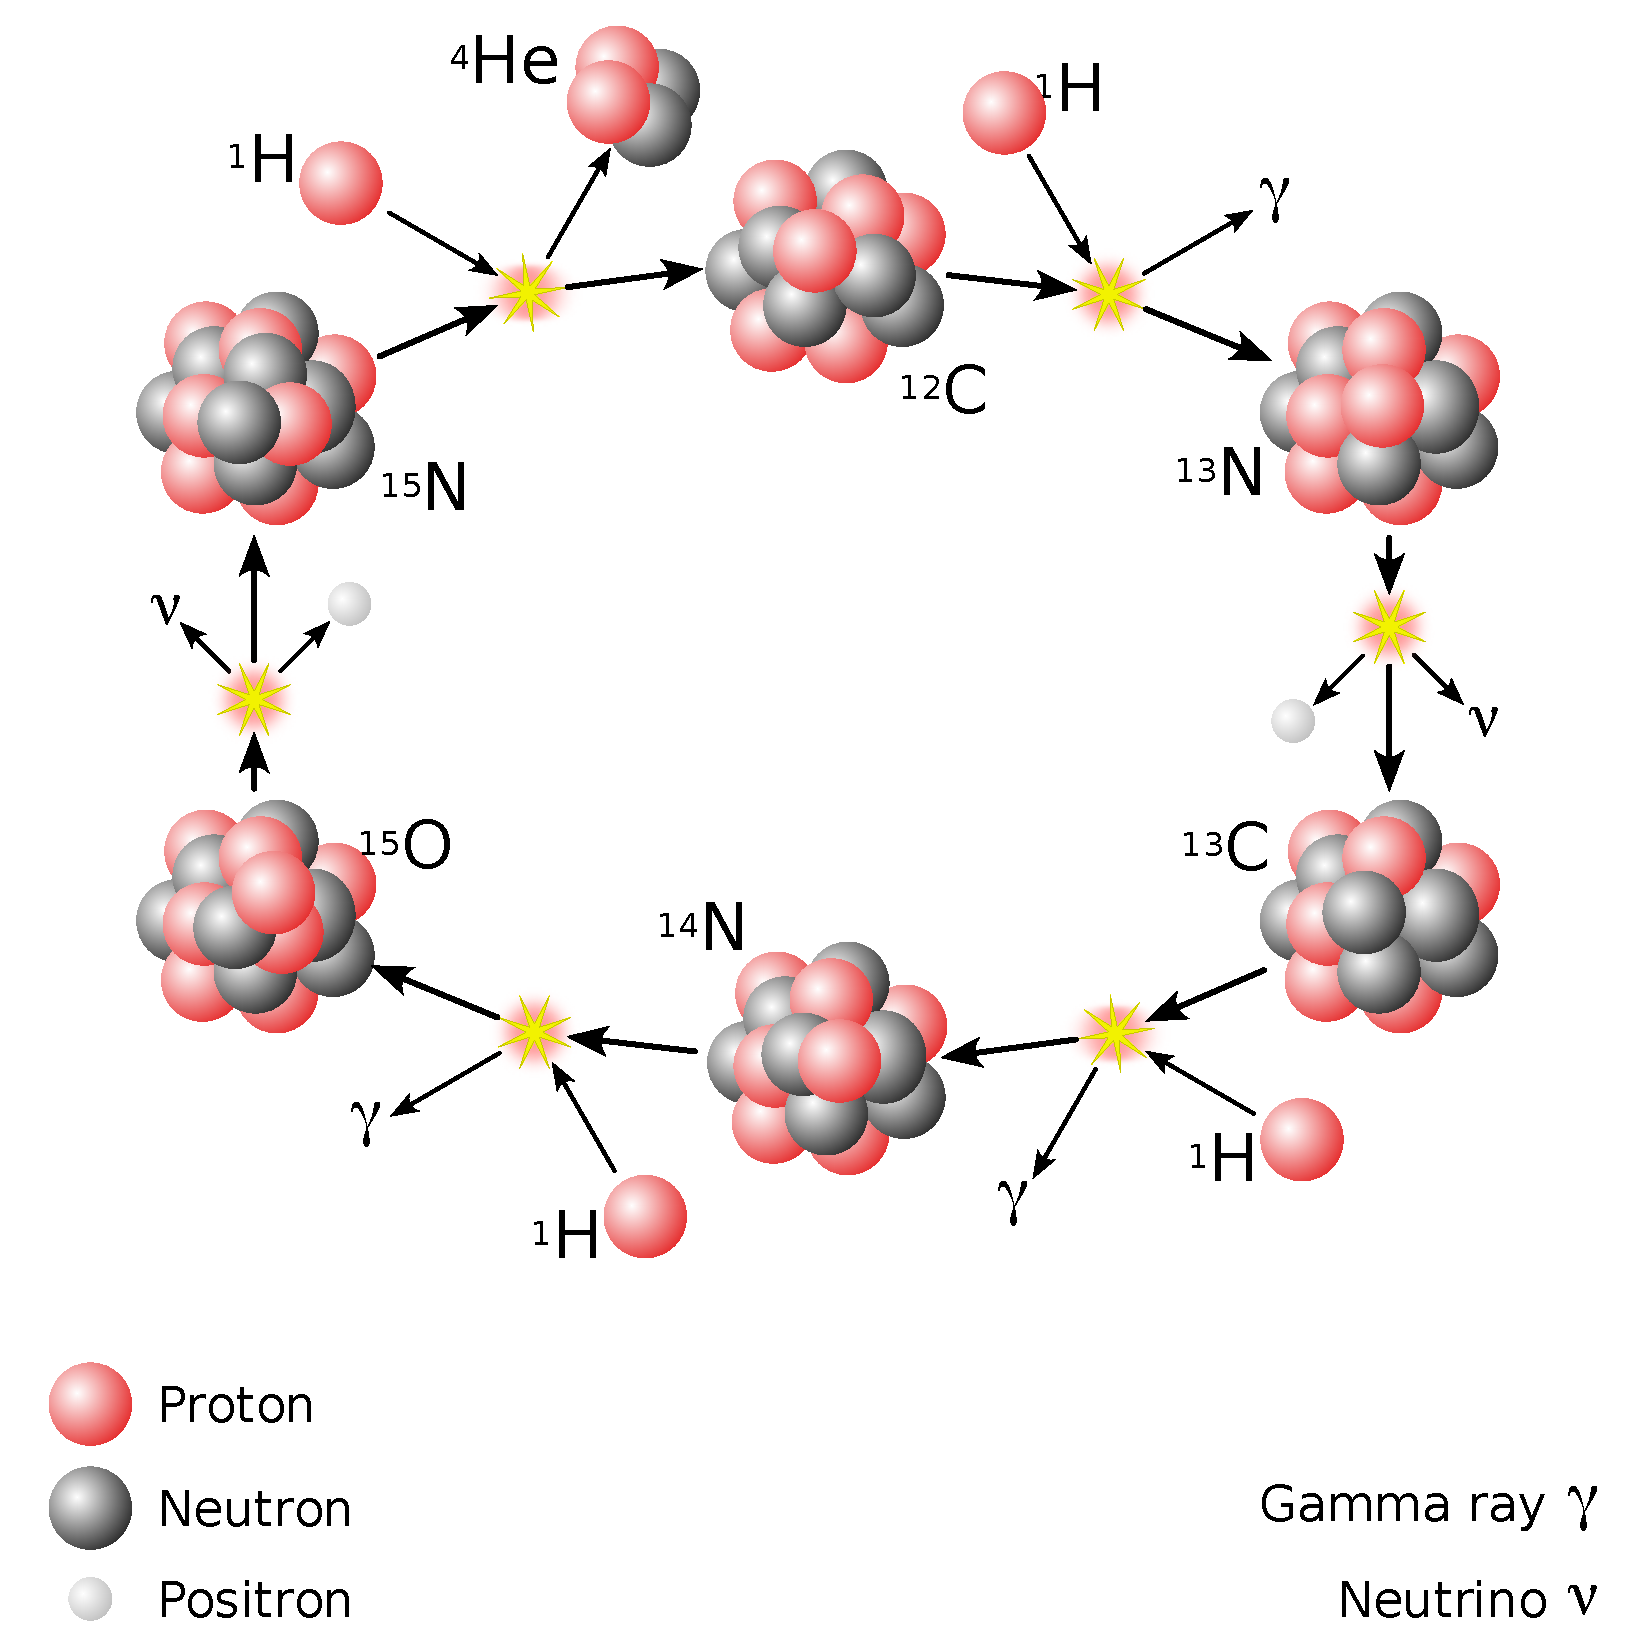
\includegraphics[width=0.4\textwidth]{img/CNO_Cycle.png}}
\end{frame}
	%metter	
	
	\begin{frame}{Astrofisica nucleare sotterranea}
		\begin{itemize}
			\item<1-> Nelle stelle, le reazioni di fusione avvengono ad energie molto inferiori rispetto alla barriera coulombiana
%			\item<2-> Sezioni d'urto molto piccole (nb-fb) implicano segnale atteso molto minore rispetto al rumore di fondo in superficie: vogliamo minimizzarlo
			\item<2-> La \emph{sezione d'urto} di una reazione nucleare è una grandezza utilizzata per descrivere la probabilità che la reazione avvenga.
			\item<4-> La si può calcolare sperimentalmente come:
			\begin{equation}
				\sigma = \dfrac{N_{reaz}/\Delta t}{N_{proj}/\Delta t \times N_{bers}/A \times \varepsilon}
			\end{equation}
			\item<5-> Con una $\sigma \approx 10^{-12}$ barn si ha un \emph{reaction rate} ($N_{reaz}/\Delta t$) che vale appena $1\div 10$ conteggi al giorno \only<6->{$\implies$ misure sotterranee}
		\end{itemize}
		
		\begin{columns}%a sinistra italia, a destra laboratori
			%al posto di cartina fondo
			\begin{column}{0.4\textwidth}
				\only<3-6>{\centering
					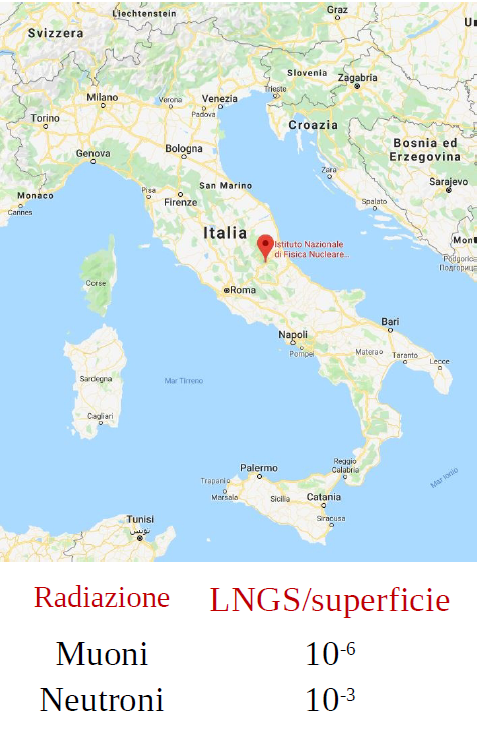
\includegraphics[width=0.4\textwidth]{img/location.png}}
				\only<7->{\centering
					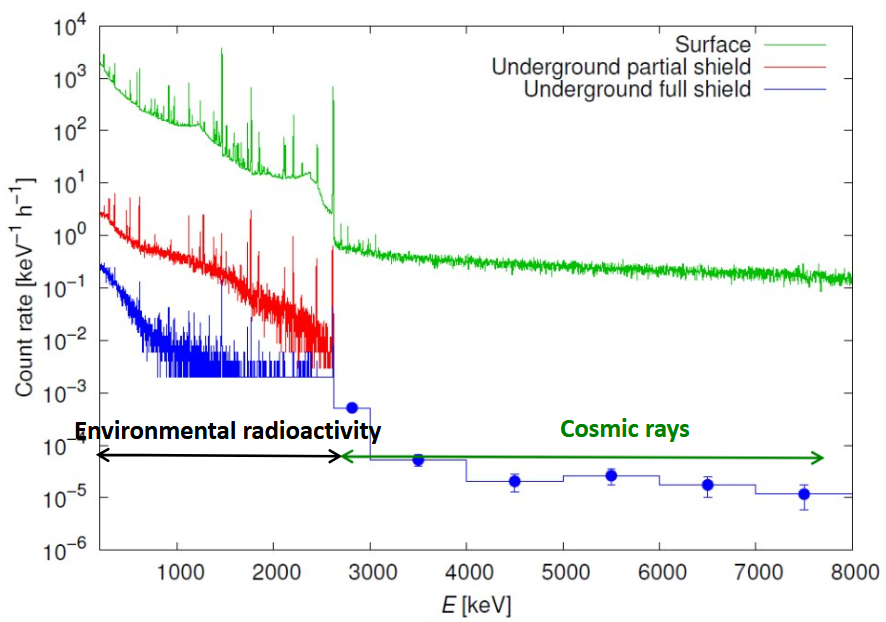
\includegraphics[width=0.8\textwidth]{img/noise.png}}
			\end{column}
			\begin{column}{0.55\textwidth}
				\uncover<6->{\centering
					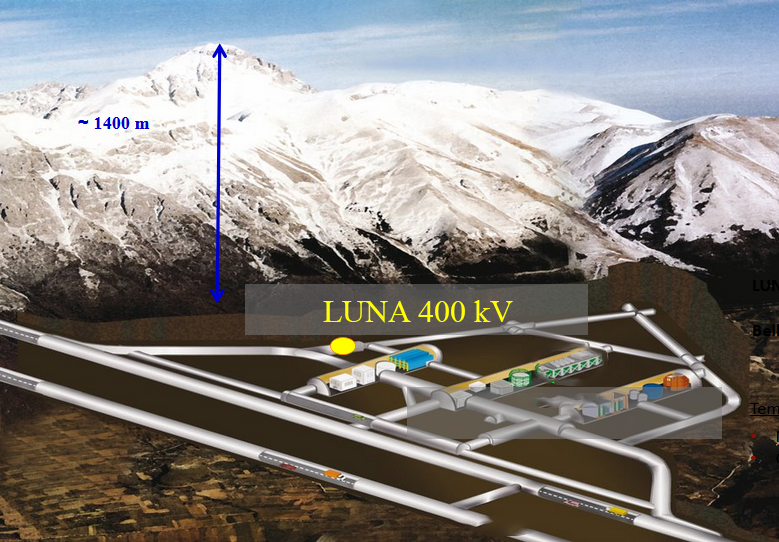
\includegraphics[width=0.6\textwidth]{img/labs.png}}
			\end{column}
			
		\end{columns}
	\end{frame}%rivedere, cartina troppo piccola
	
%\begin{frame}{Sfide sperimentali della misura diretta}
%	\begin{itemize}
%		
%		%A VOCE
%		%	\item<3-> $N_{reaz}/\Delta t$ è il numero di reazioni per unità di tempo;
%		%	\item<4-> $N_{proj}/\Delta t \approx 10^{14}$ pps per intensità tipiche di un fascio stabile
%		%	\item<5-> $N_{bers}/A \approx 10^{19}$ atomi/cm per un tipico bersaglio allo stato solido
%		%	\item<6-> $\sigma \approx 10^{-12}$ barn, spesso è anche più piccola
%		%	\item<7-> $\varepsilon \approx 1 \div 10 \%$ per i raggi gamma
%	\end{itemize}
%\end{frame}

	
\begin{frame}{LUNA 400 kV}%spiegare a voce
	\centering
	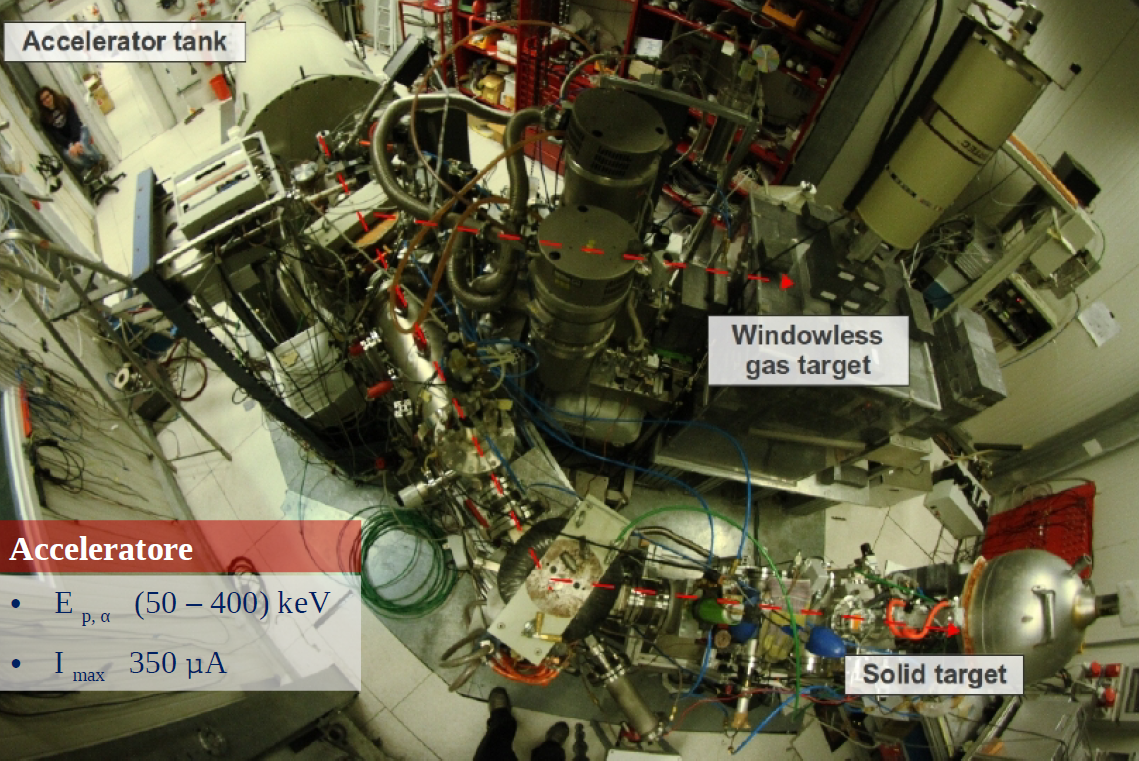
\includegraphics[width=0.9\textwidth]{img/LUNA2.png}
	\captionof{figure}{Apparato sperimentale LUNA.}
\end{frame}

%\begin{frame}{Apparato sperimentale}
%	%immagine 3d del bgo
%	%bersaglio solido in TiN (immagine sul'elog)
%	%si tratta di un reivelatore...
%	%la seconda a voce
%	\begin{columns}
%		\begin{column}{0.35\textwidth}
%			\begin{itemize}
%				%\item La radiazione gamma emessa dalla reazione è rivelata da uno scintillatore.
%				\item<1-> Fascio di protoni 50-400 keV
%				\item<2-> Bersaglio solido TiN ()
%				
%				\item<3-> Rivelatore di fotoni: BGO % a voce:, coprente il 95\% dell'angolo solido totale attorno al bersaglio.
%				%a voce: È otticamente diviso in sei spicchi
%				 
%				\item<4-> Segnali in uscita letti da digitizer  CAEN
%				%densità atomica del TiN in atomi/cm^2
%				%parlare della catena elettronica
%				%otticamente diviso in sei spicchi
%				%si leggonon con un digitizer delal caen (modello) e c'è anche un pulser
%				
%				
%%				\item Si tratta di uno scintillatore, ossia uno strumento che quando eccitato da radiazione ionizzante, ne assorbe l'energia depositata e la riemette sotto forma di fotoni
%			\end{itemize}
%		\end{column}%primo bersaglio solido
%	%poi bgo 3d
%	%poi bgo 2d
%	%poi catena (più grande)
%		\begin{column}{0.65\textwidth}
%			\only<1>{\centering
%				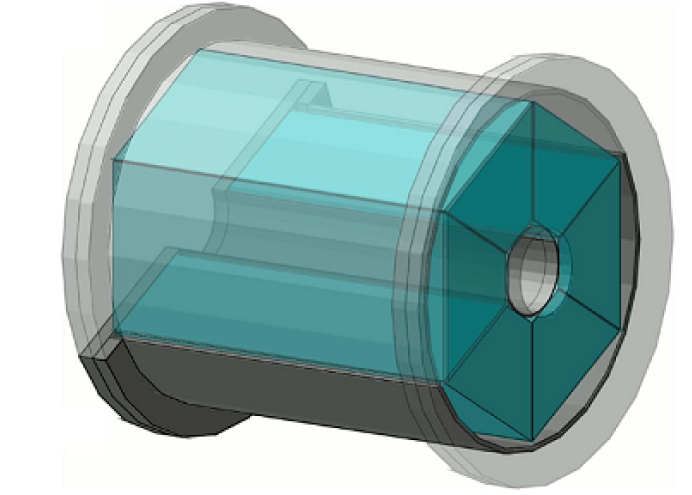
\includegraphics[width=0.6\textwidth]{img/bgo_3d.png}}
%			\uncover<2->{\centering
%				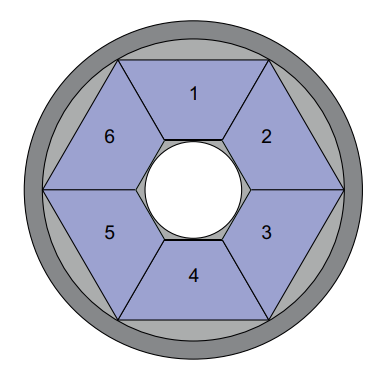
\includegraphics[width=0.6\textwidth]{img/bgo_cross.png}}
%			%\captionof{figure}{Rappresentazione 3D del rivelatore BGO.}
%			\uncover<3>{\centering
%				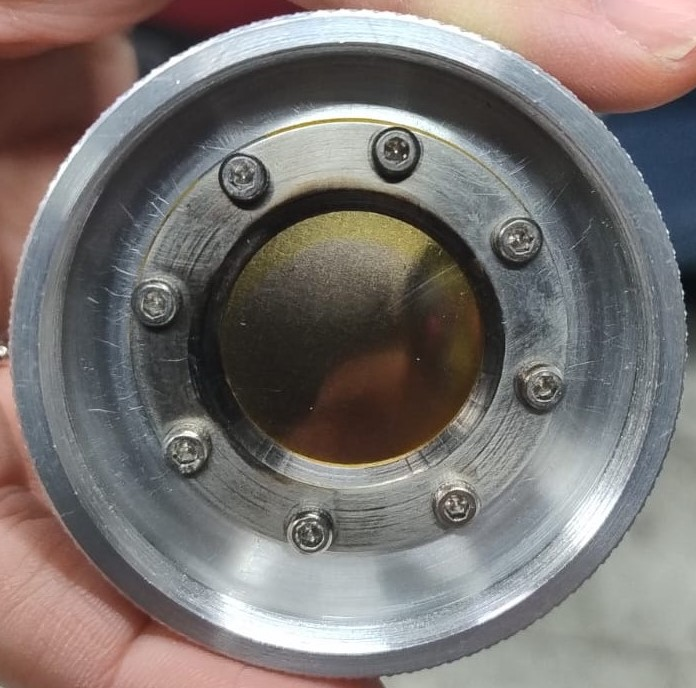
\includegraphics[width=0.8\textwidth]{img/tin.jpg}}
%			\only<4->{\centering
%				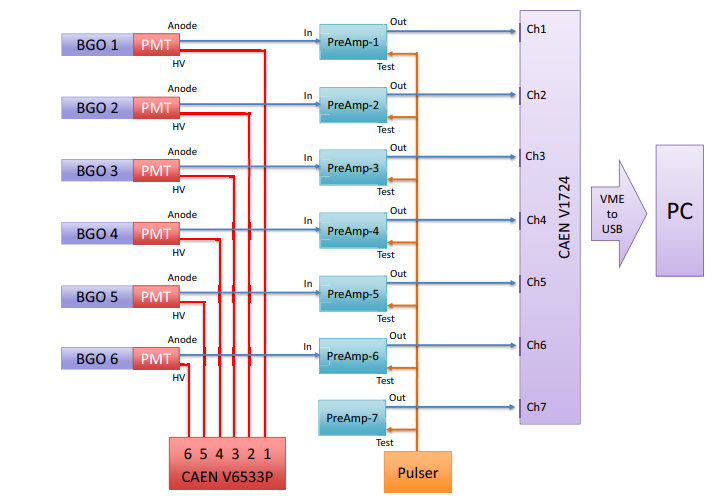
\includegraphics[width=0.5\textwidth]{img/electronics.png}}
%		\end{column}
%	\end{columns}
%\end{frame}

\begin{frame}{Apparato sperimentale}
	\begin{columns}
		\begin{column}{0.35\textwidth}
			\begin{itemize}
				\item<1-> Fascio di protoni 50-400 keV
				\item<2-> Bersaglio solido TiN
				\item<3-> Rivelatore di fotoni: BGO
				\item<5-> Segnali in uscita letti da digitizer CAEN
			\end{itemize}
		\end{column}
		
		\begin{column}{0.65\textwidth}
			% Top image placeholder (shows in slides 1, replaced in slide 3)
			\only<2-3>{\centering
				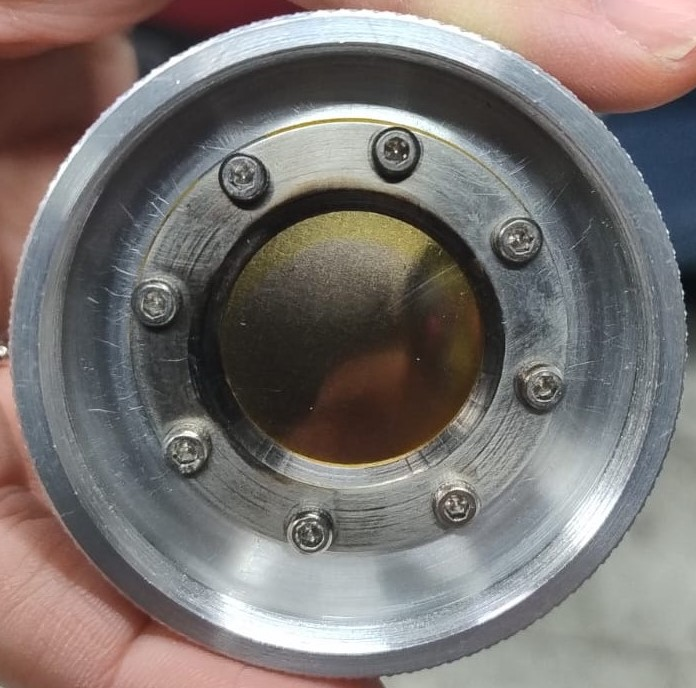
\includegraphics[width=0.5\textwidth]{img/tin.jpg}}
			\only<4->{\centering
				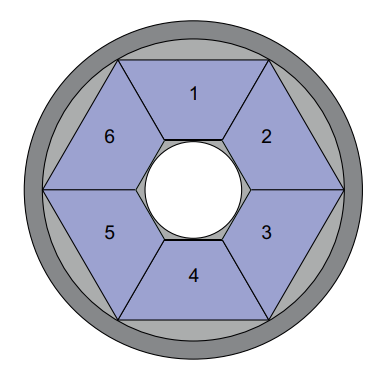
\includegraphics[width=0.3\textwidth]{img/bgo_cross.png}}
			
			\vspace{0.5cm} % Adjust the space as needed to reserve for bottom image
			
			% Bottom image (appears on slide 2, then gets replaced on slide 4)
			\only<3-4>{\centering
				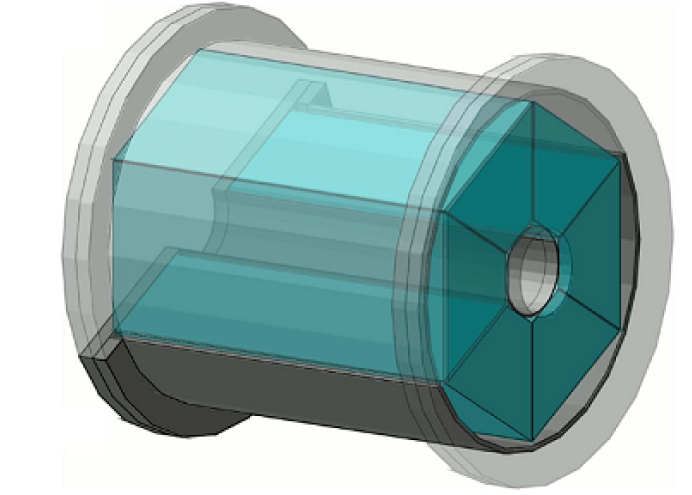
\includegraphics[width=0.6\textwidth]{img/bgo_3d.png}}
			\only<5->{\centering
				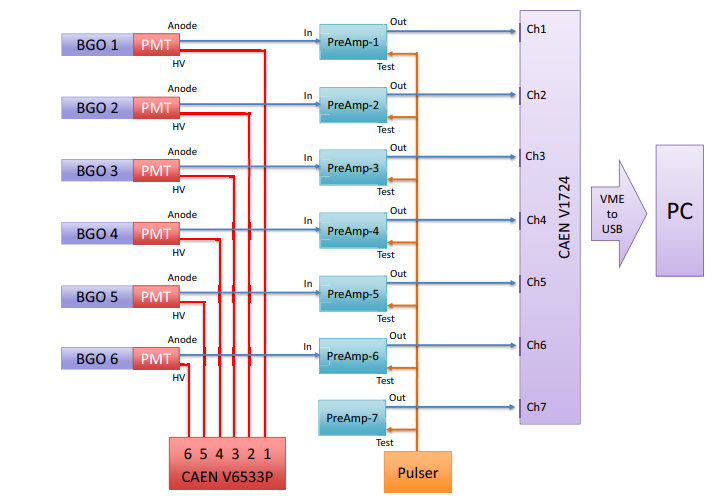
\includegraphics[width=0.9\textwidth]{img/electronics.png}}
		\end{column}
	\end{columns}
\end{frame}





	\section{Obiettivi della tesi}
	\begin{frame}{Obiettivi della tesi}
	L'obiettivo della tesi, incentrato sull'analisi dei dati, è quello di 	
		\begin{itemize}%mettere schematicamente, punto per efficienza e punto per energia
			\item<2-> calibrare in energia 
			\item<3-> caratterizzare in efficienza 
		\end{itemize}
	\uncover<4->{lo scintillatore.}\\
		
		\uncover<5->{L'analisi dei dati viene confrontata con delle simulazioni in GEANT4.}
	\end{frame}



\section{Calibrazione in energia}
\begin{frame}{Calibrazione in energia}
	\begin{itemize}
		\item Viene effettuata con due sorgenti radioattive, $^{137}$Cs e $^{60}$Co, ad attività nota
		%\item La calibrazione in energia consiste nel calcolo dei fattori che convertono da valori in canali (CHN) a valori in energia (keV) 
		%\item Tutta l'analisi dei dati è effettuata in ROOT, framework per l'analisi dei dati scritta in C++ e sviluppata dal CERN.
	\end{itemize}
	
	\vspace{5mm} % Adds some vertical space between the item and the images
	
	\begin{columns}
		\column{0.5\textwidth}
		\uncover<2->{\centering
			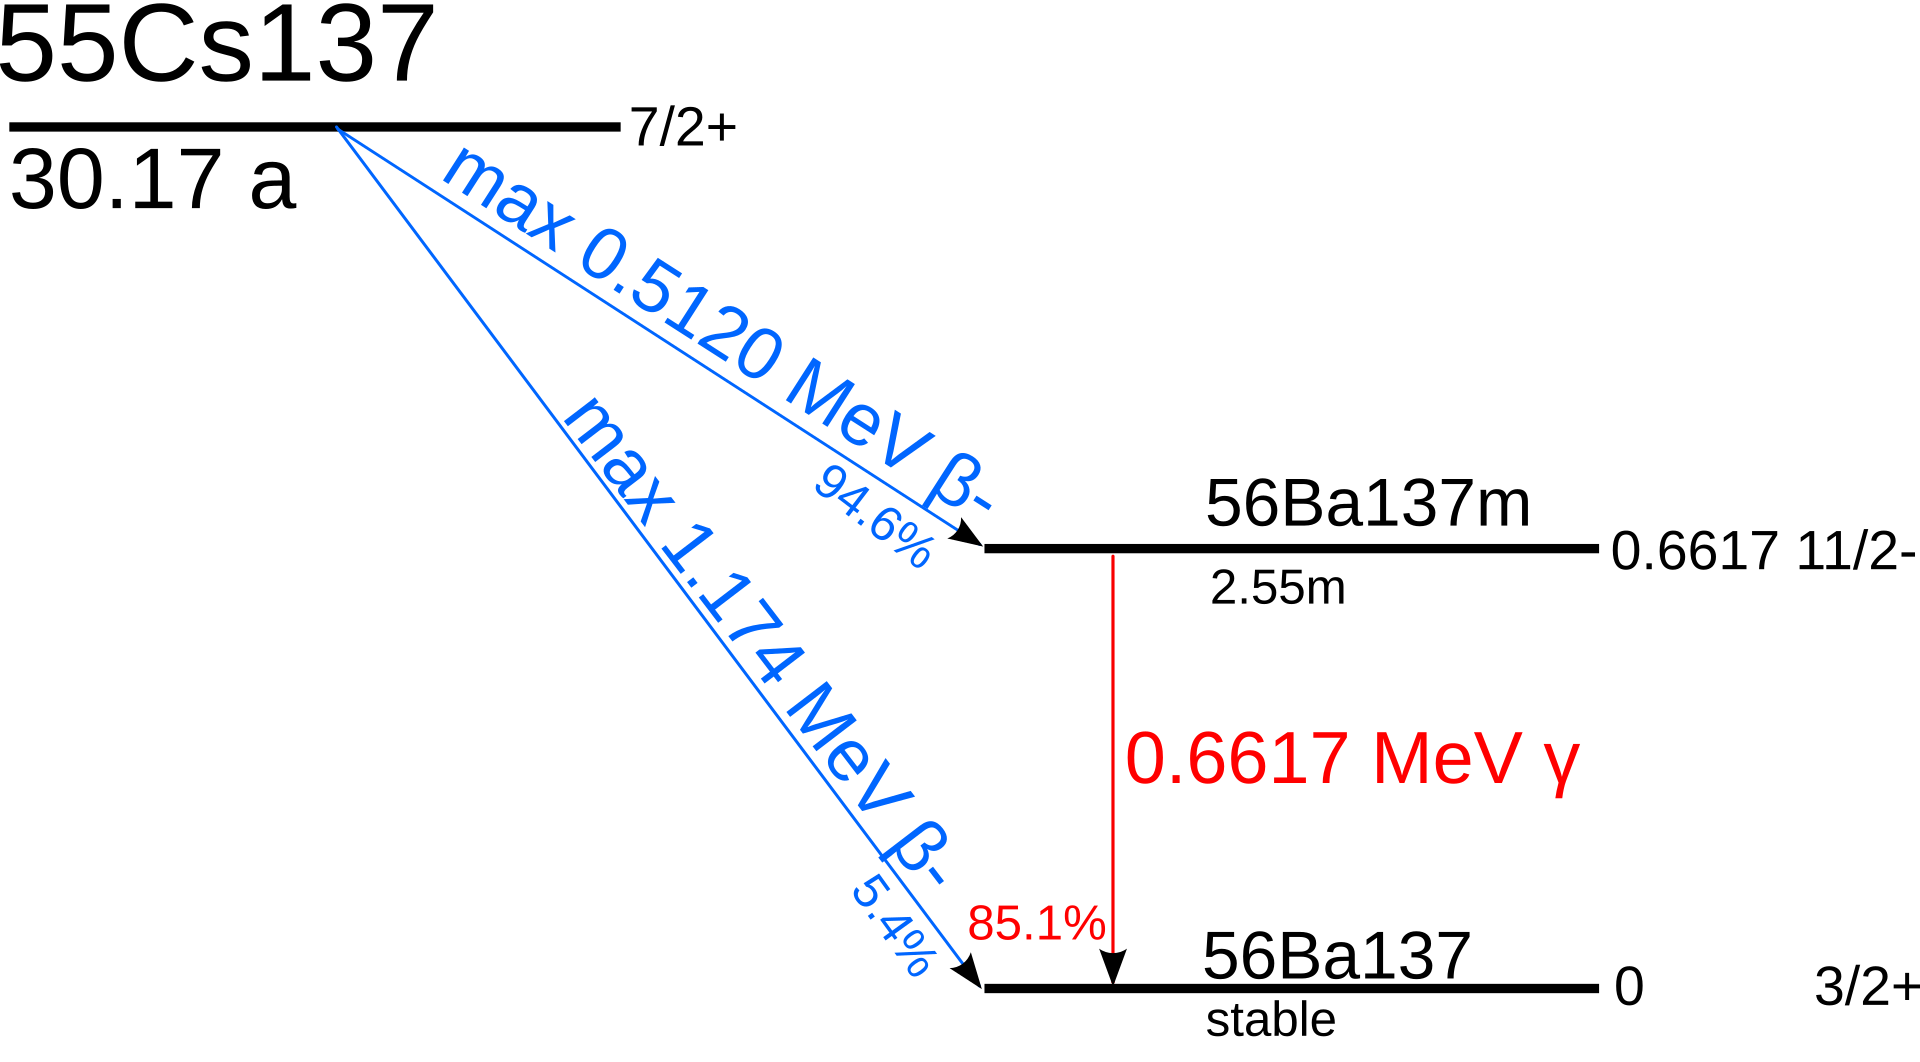
\includegraphics[width=0.9\textwidth]{img/Cs-137-decay.png}
			\centering
			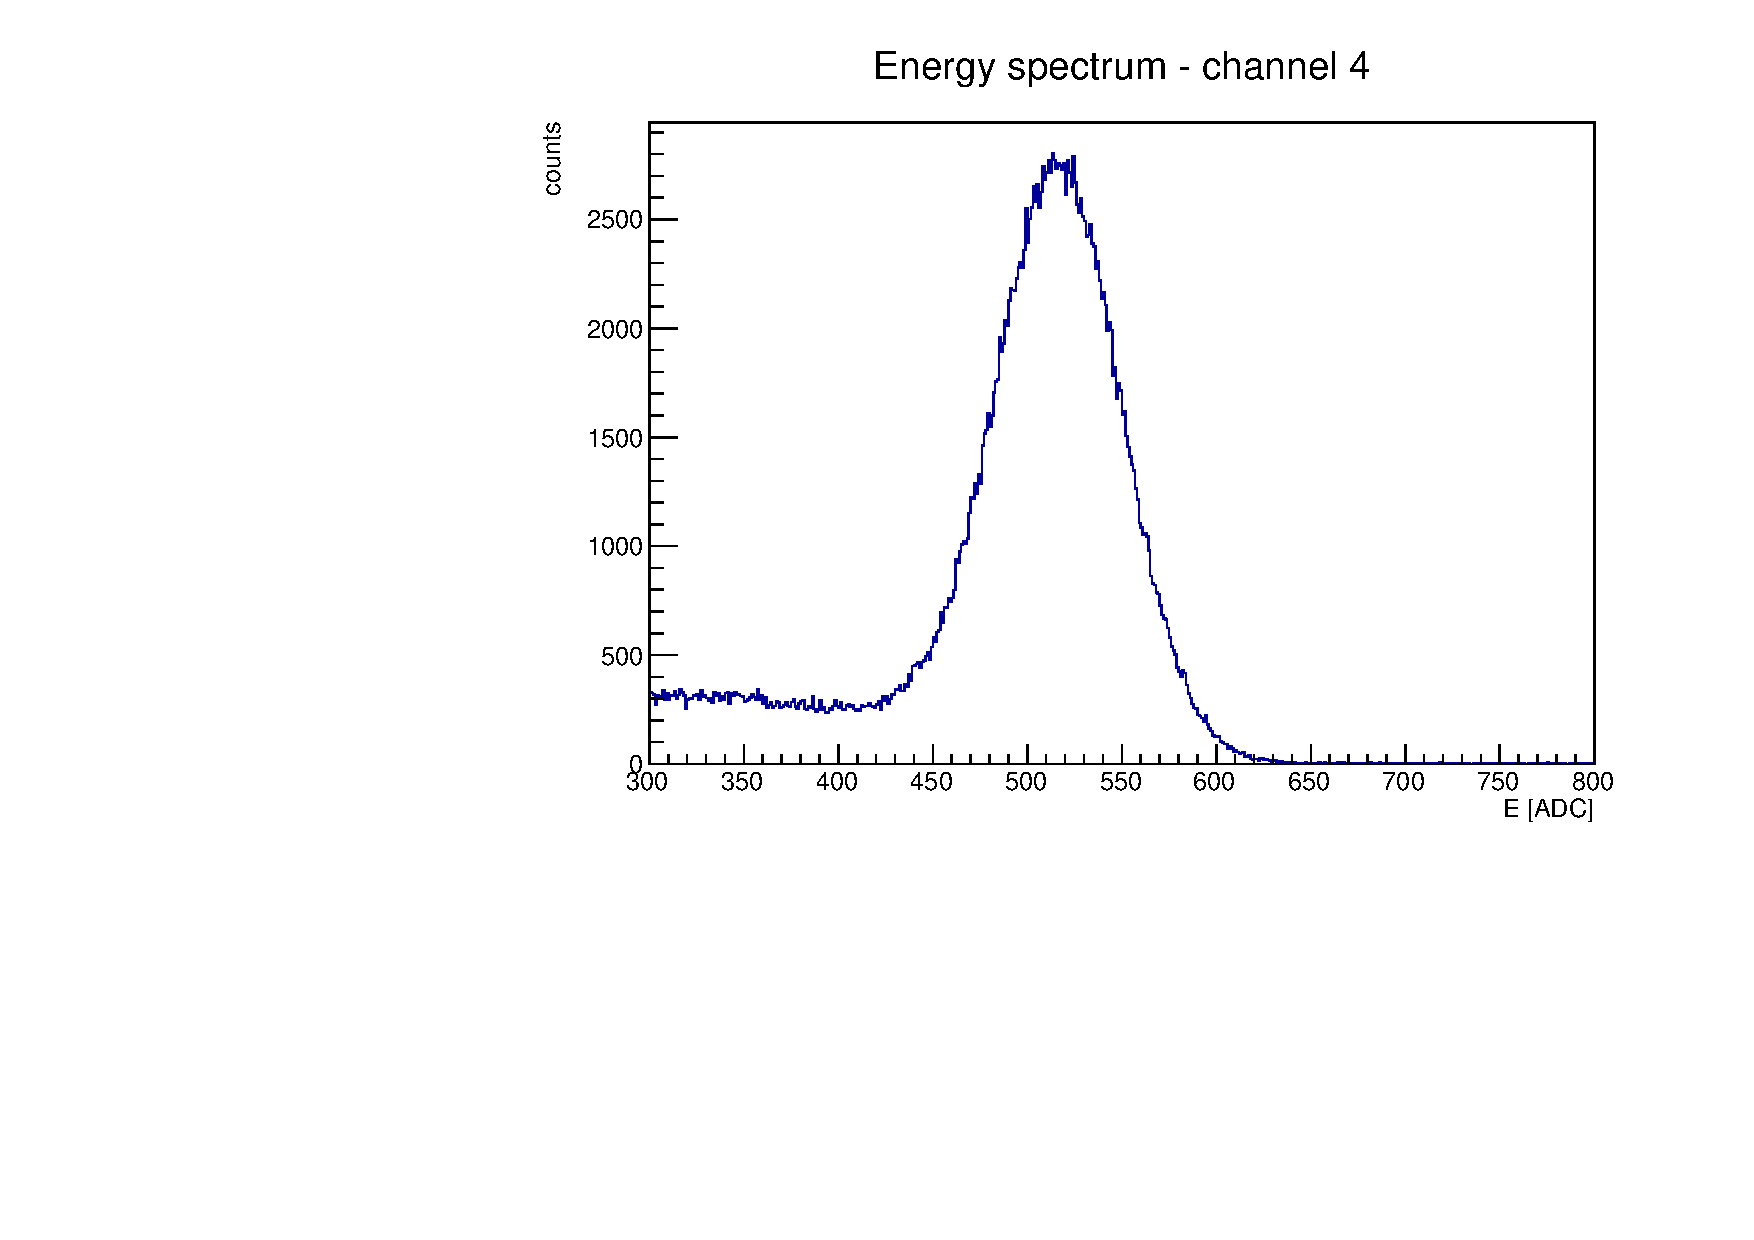
\includegraphics[width=0.9\linewidth]{img/ex1776.pdf}}
		\column{0.5\textwidth}
		\uncover<3->{\centering
			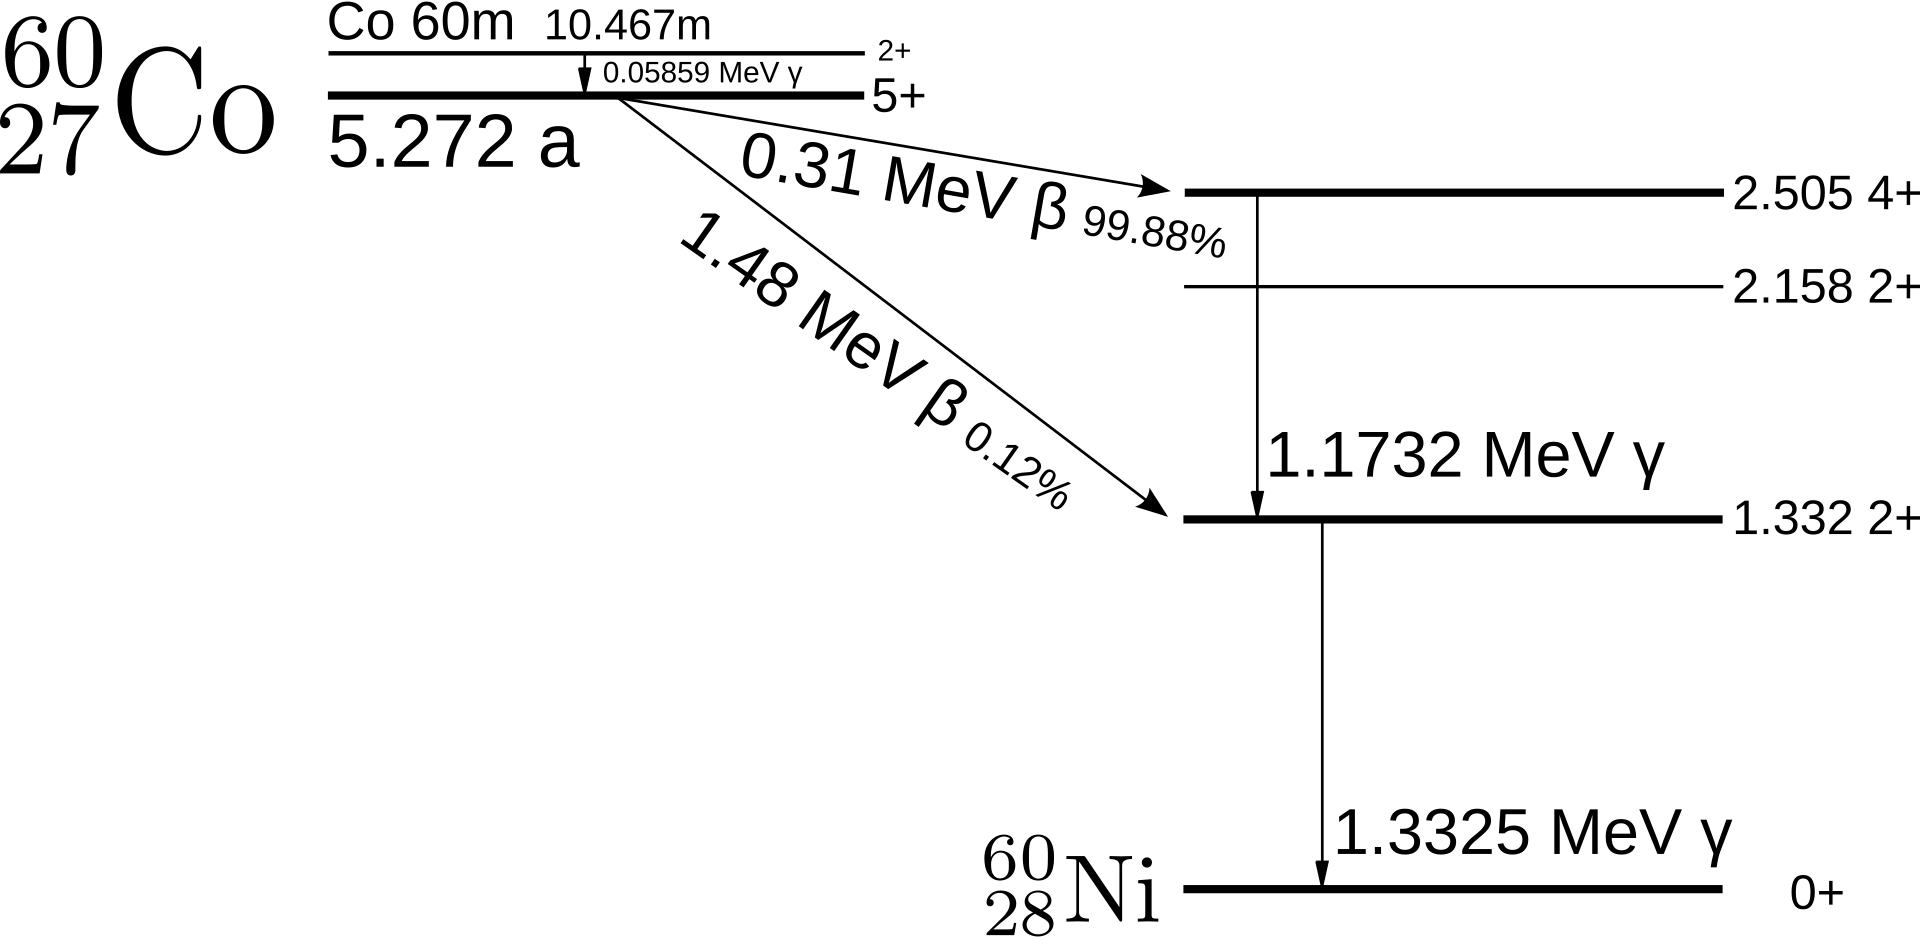
\includegraphics[width=0.95\textwidth]{img/Cobalt-60m-decay.png}
			\centering
			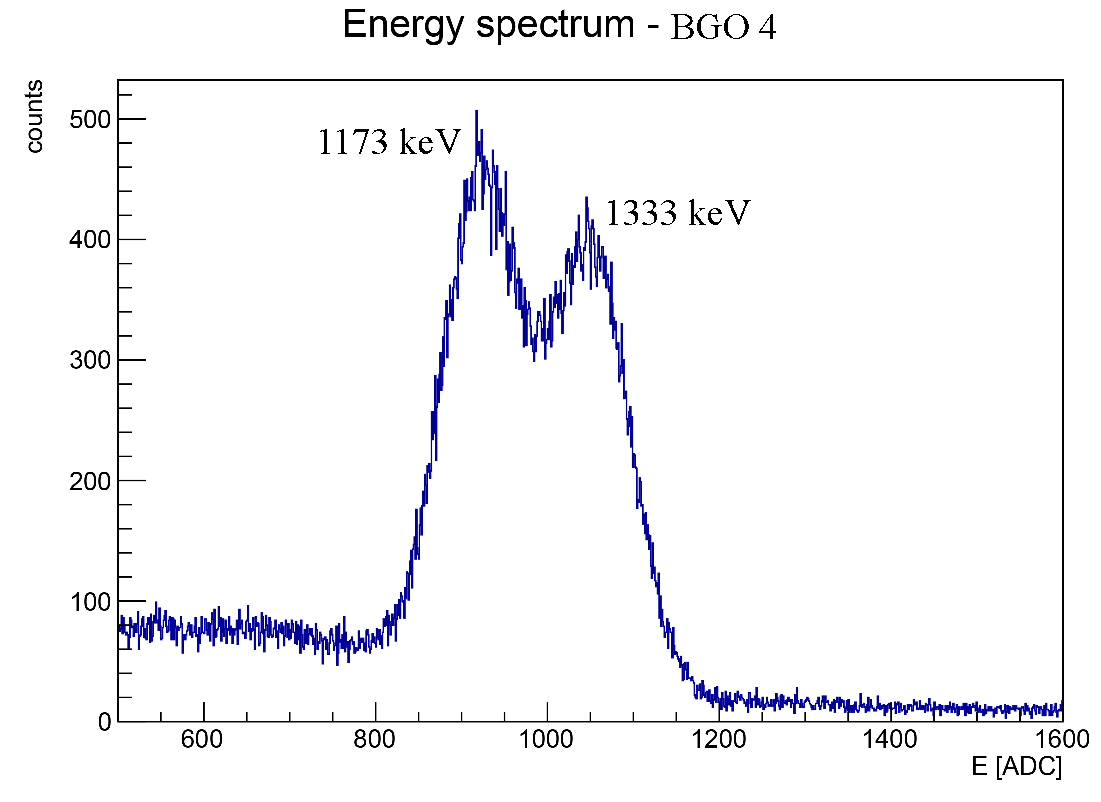
\includegraphics[width=0.9\linewidth]{img/ex1777.pdf}}
	\end{columns}
\end{frame}




%mostrare solo istrogramma calibrazione in energia
%bgo 6 segmenti, tutti analizzati
%mostrato uno solo
%mettere spicchio 4
%zoom solo fino a cobalto
%togliere riquadro in alto a sinistra

%\begin{frame}{Istogrammi}
%	\begin{figure}
%		\centering
%		\begin{minipage}{0.45\textwidth}
%			\centering
%			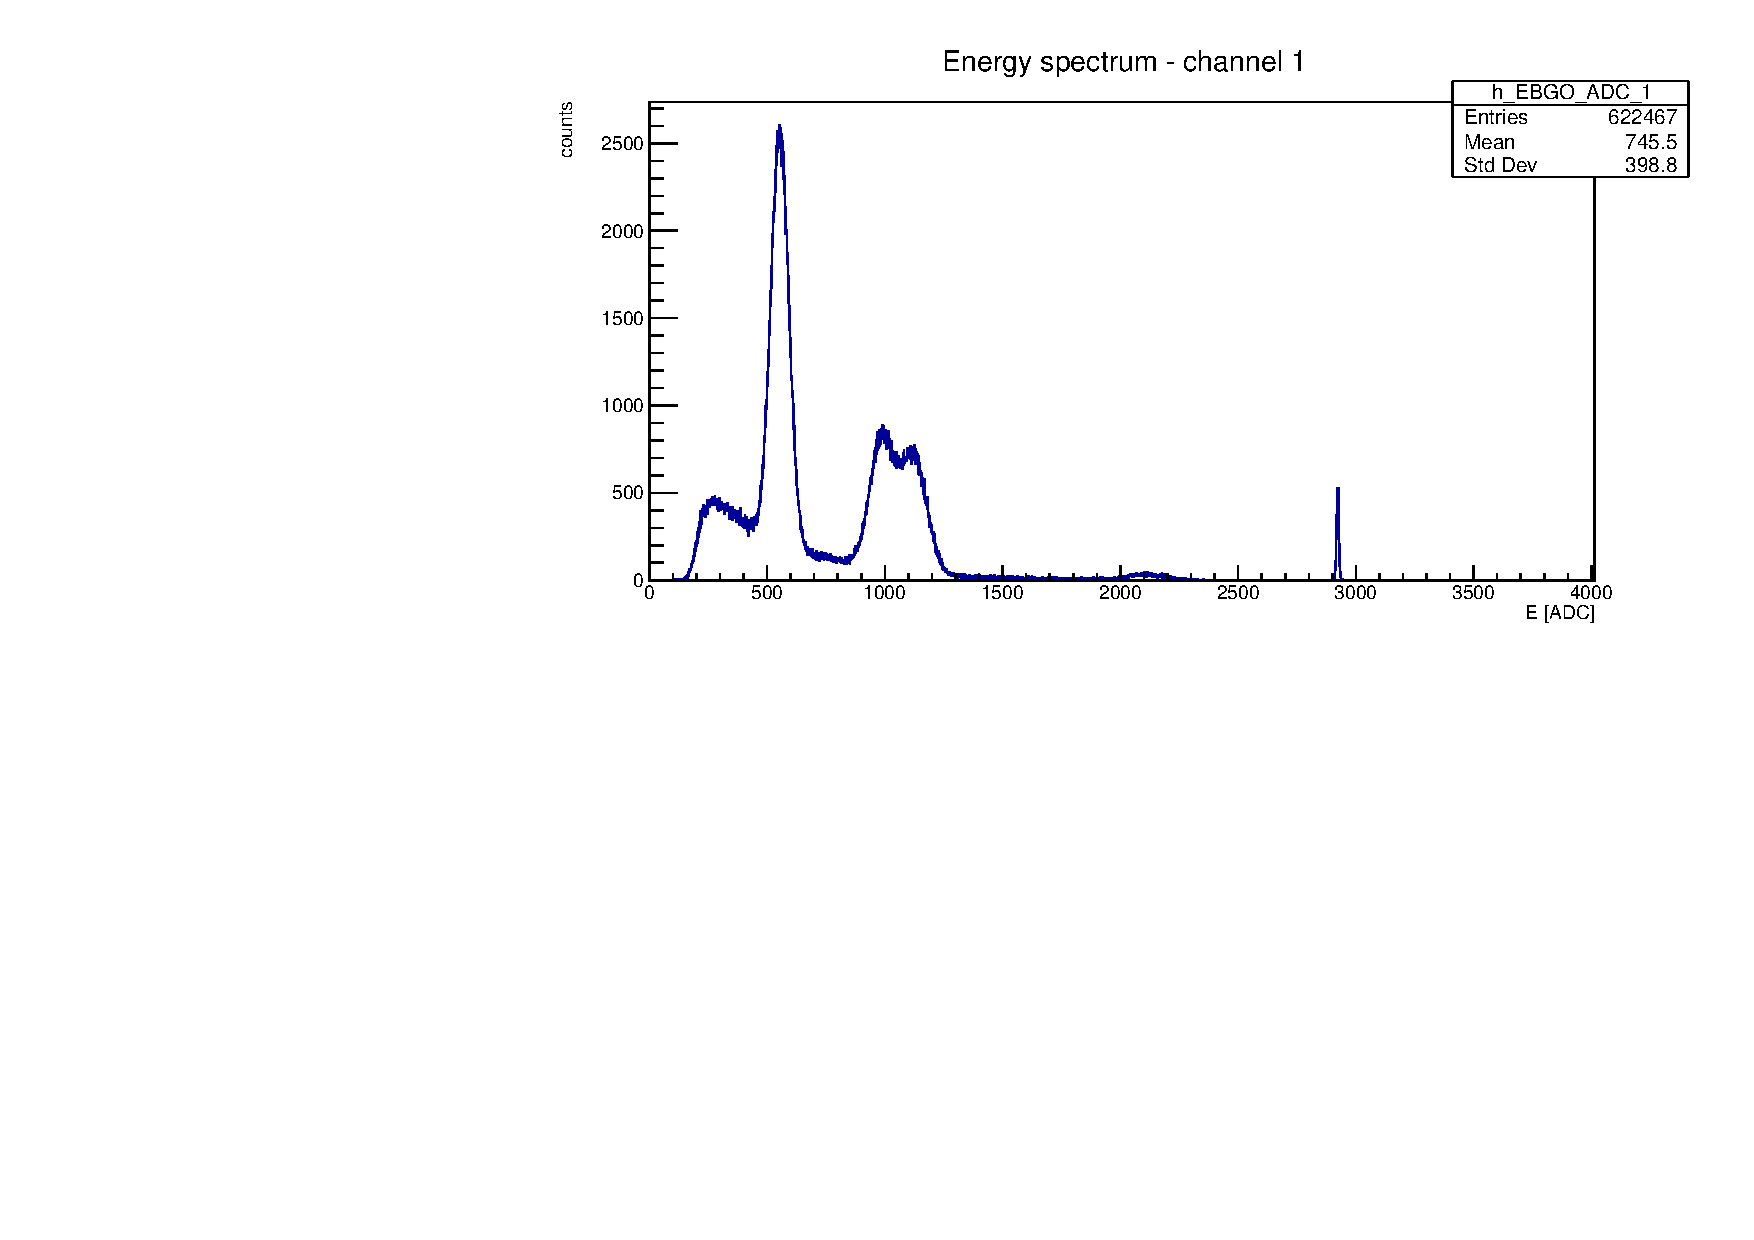
\includegraphics[width=\linewidth]{img/ex1775.pdf} % Replace with your image path
%		\end{minipage}
%		\hfill
%		\begin{minipage}{0.45\textwidth}
%			\centering
%			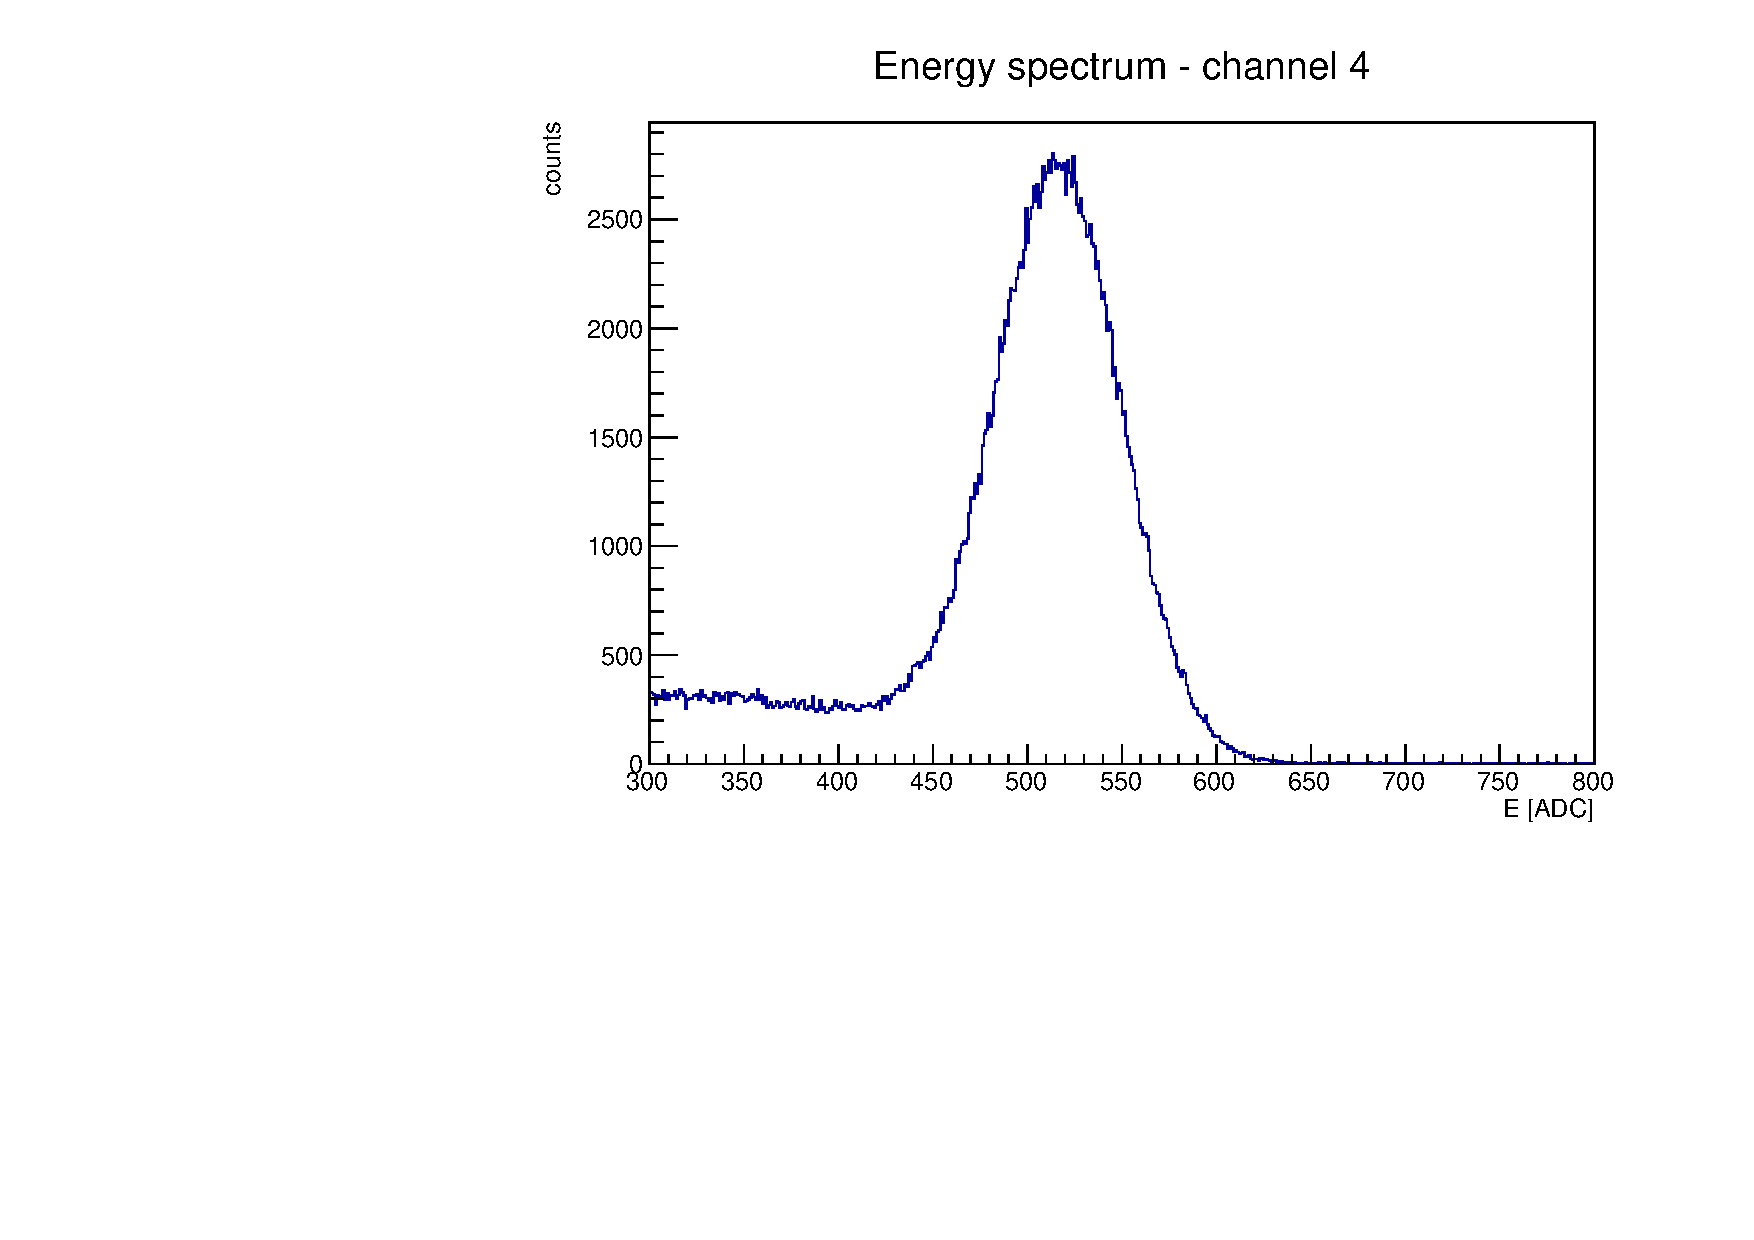
\includegraphics[width=\linewidth]{img/ex1776.pdf} % Replace with your image path
%		\end{minipage}
%		
%		\vspace{0.4cm} % Adjust vertical space between rows
%		
%		\begin{minipage}{0.45\textwidth}
%			\centering
%			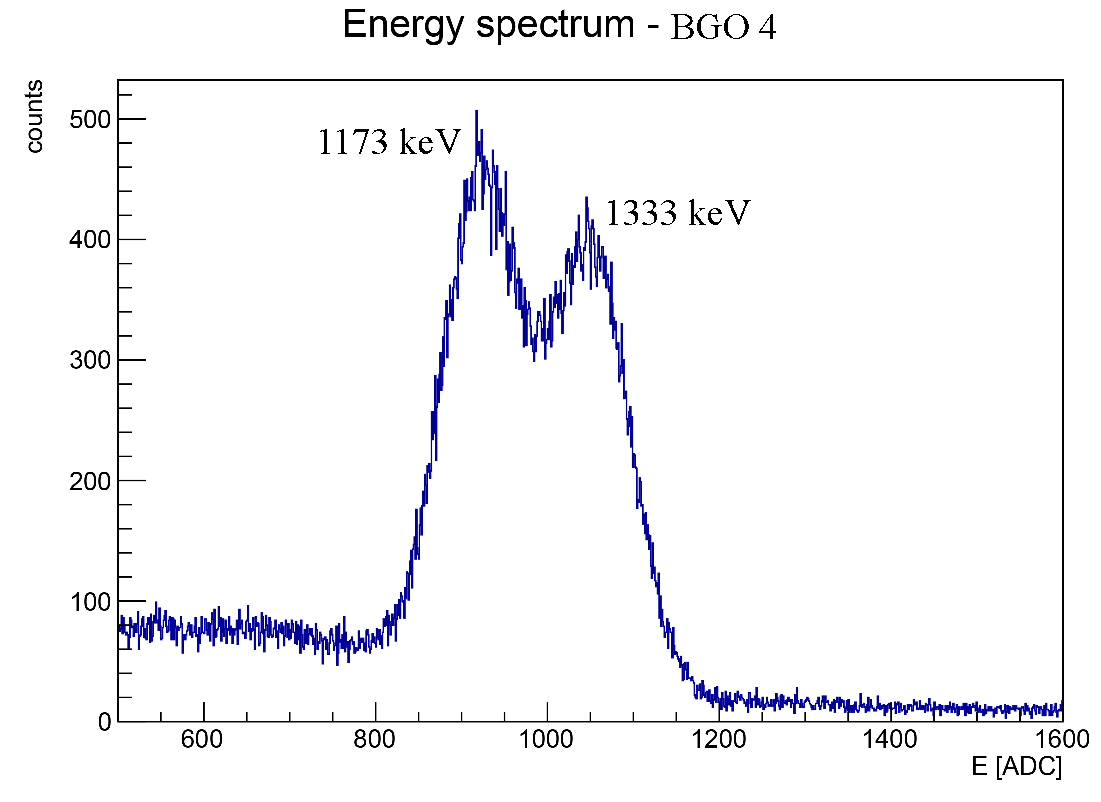
\includegraphics[width=\linewidth]{img/ex1777.pdf} % Replace with your image path
%		\end{minipage}
%		\hfill
%		\begin{minipage}{0.45\textwidth}
%			\centering
%			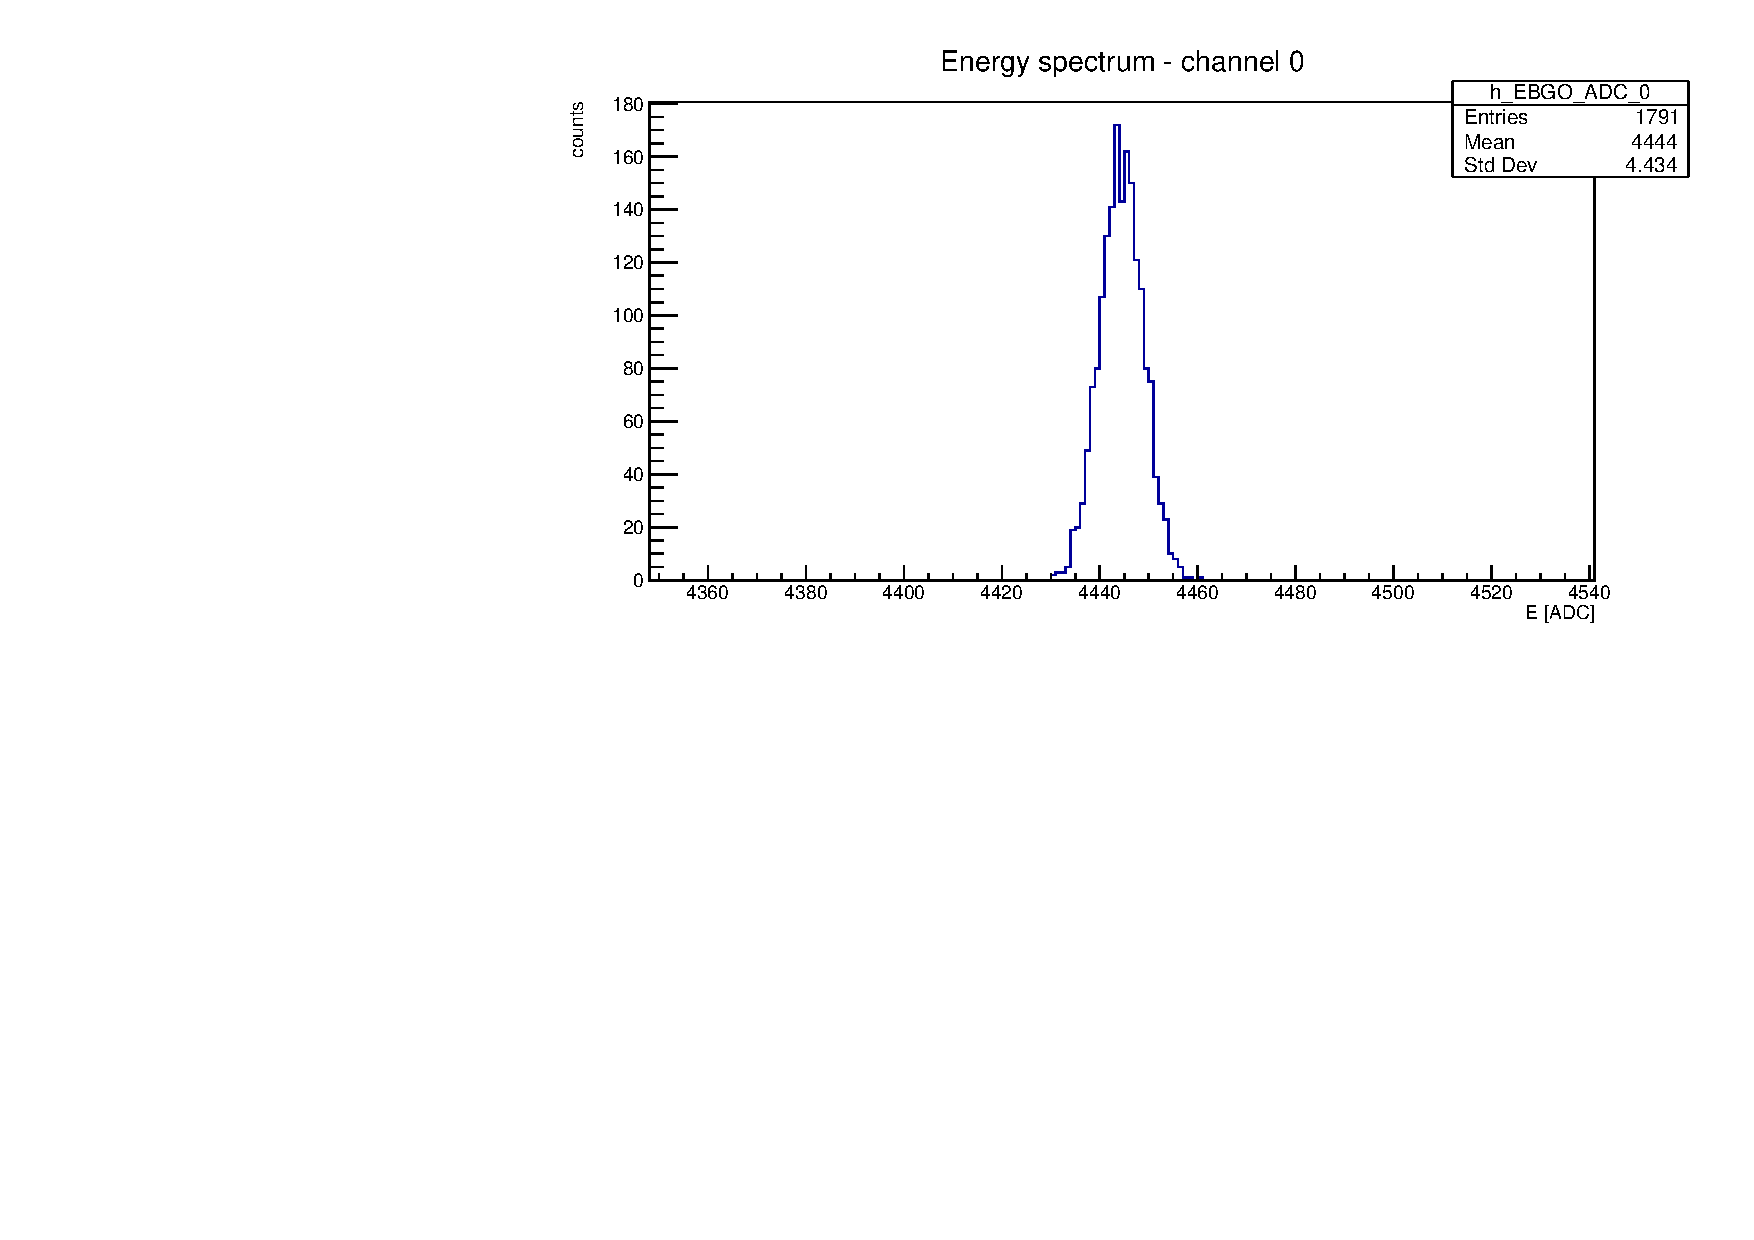
\includegraphics[width=\linewidth]{img/pulser.pdf} % Replace with your image path
%		\end{minipage}
%	\end{figure}
%\end{frame}

\begin{frame}{Calcolo della calibrazione}
	\begin{columns}%mettere foto istogramma spicchio 4 con due elementi
		\begin{column}{0.45\textwidth}% a voce
%			\begin{itemize}
%				\item<1-> Si effettuano fit sui file con entrambe le sorgenti
%				\item<2-> I valori dei picchi vengono graficati contro quelli in energia caratteristici, noti.
%				\item<4-> Si effettua dunque un fit lineare per i punti di ciascun istogramma.
%				\item<5-> I coefficienti angolari di questi fit sono i fattori di conversione cercati.
%			\end{itemize}
			%chiamare secondo grafico con "Energy" anziché Energy calibration
				%Cambiare nome "BGO 4" anziché graph 4
				\centering
				\only<1->{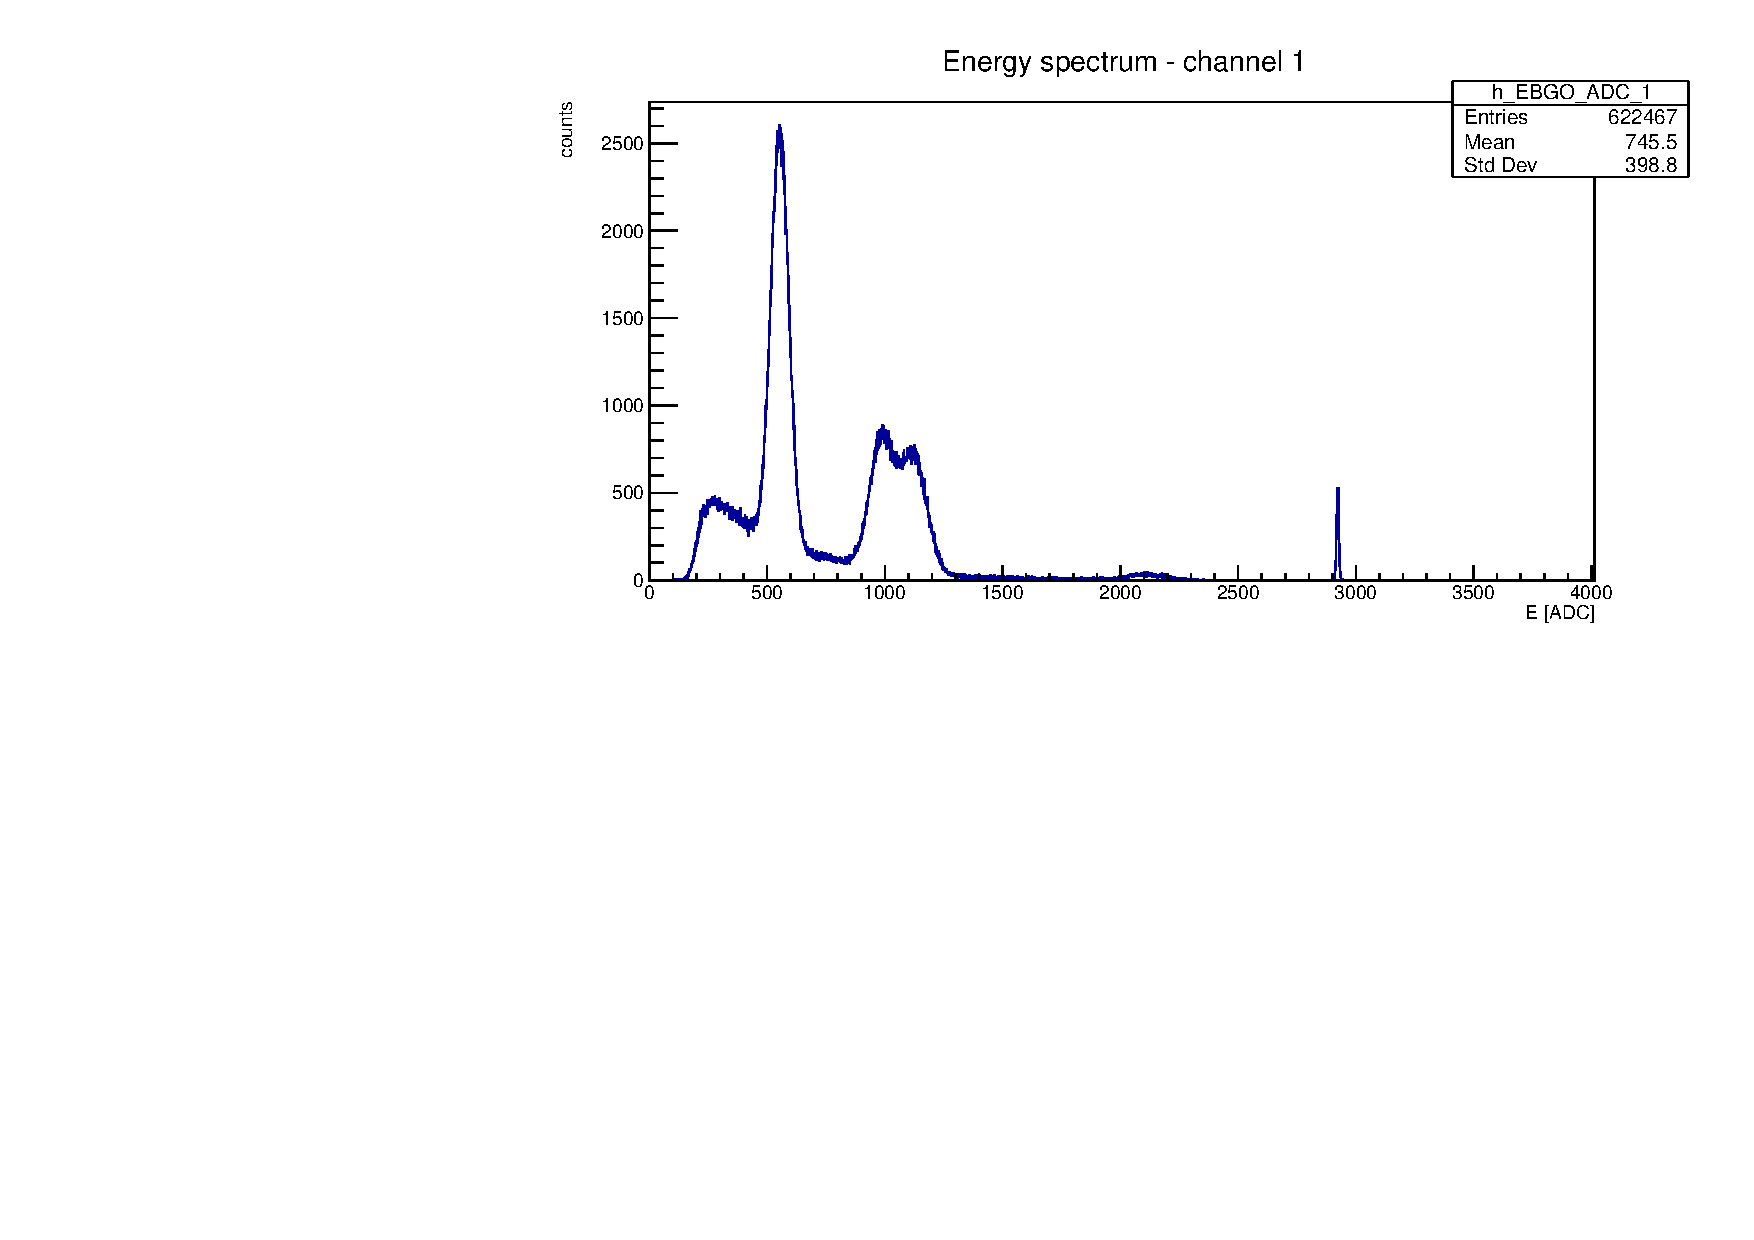
\includegraphics[width=0.95\linewidth]{img/ex1775.pdf}}
				\uncover<4->{\begin{figure}
						\begin{table}[ht!]
						\centering
						\resizebox{0.9\textwidth}{!}{
							\begin{tabular}{@{}cccc@{}}
								\toprule
								Canale & a [keV] & b [keV/CHN] \\ \midrule
								CHN4 & 5.83 \(\pm\) 0.39 & 1.2676 \(\pm\) 0.0006 \\
								\bottomrule
						\end{tabular}}
				\end{table}\end{figure}}
				%SISTEMARE LìORDINE DEI GRAFICI
			
		\end{column}
		\begin{column}{0.45\textwidth}
			
				\centering
				\only<2>{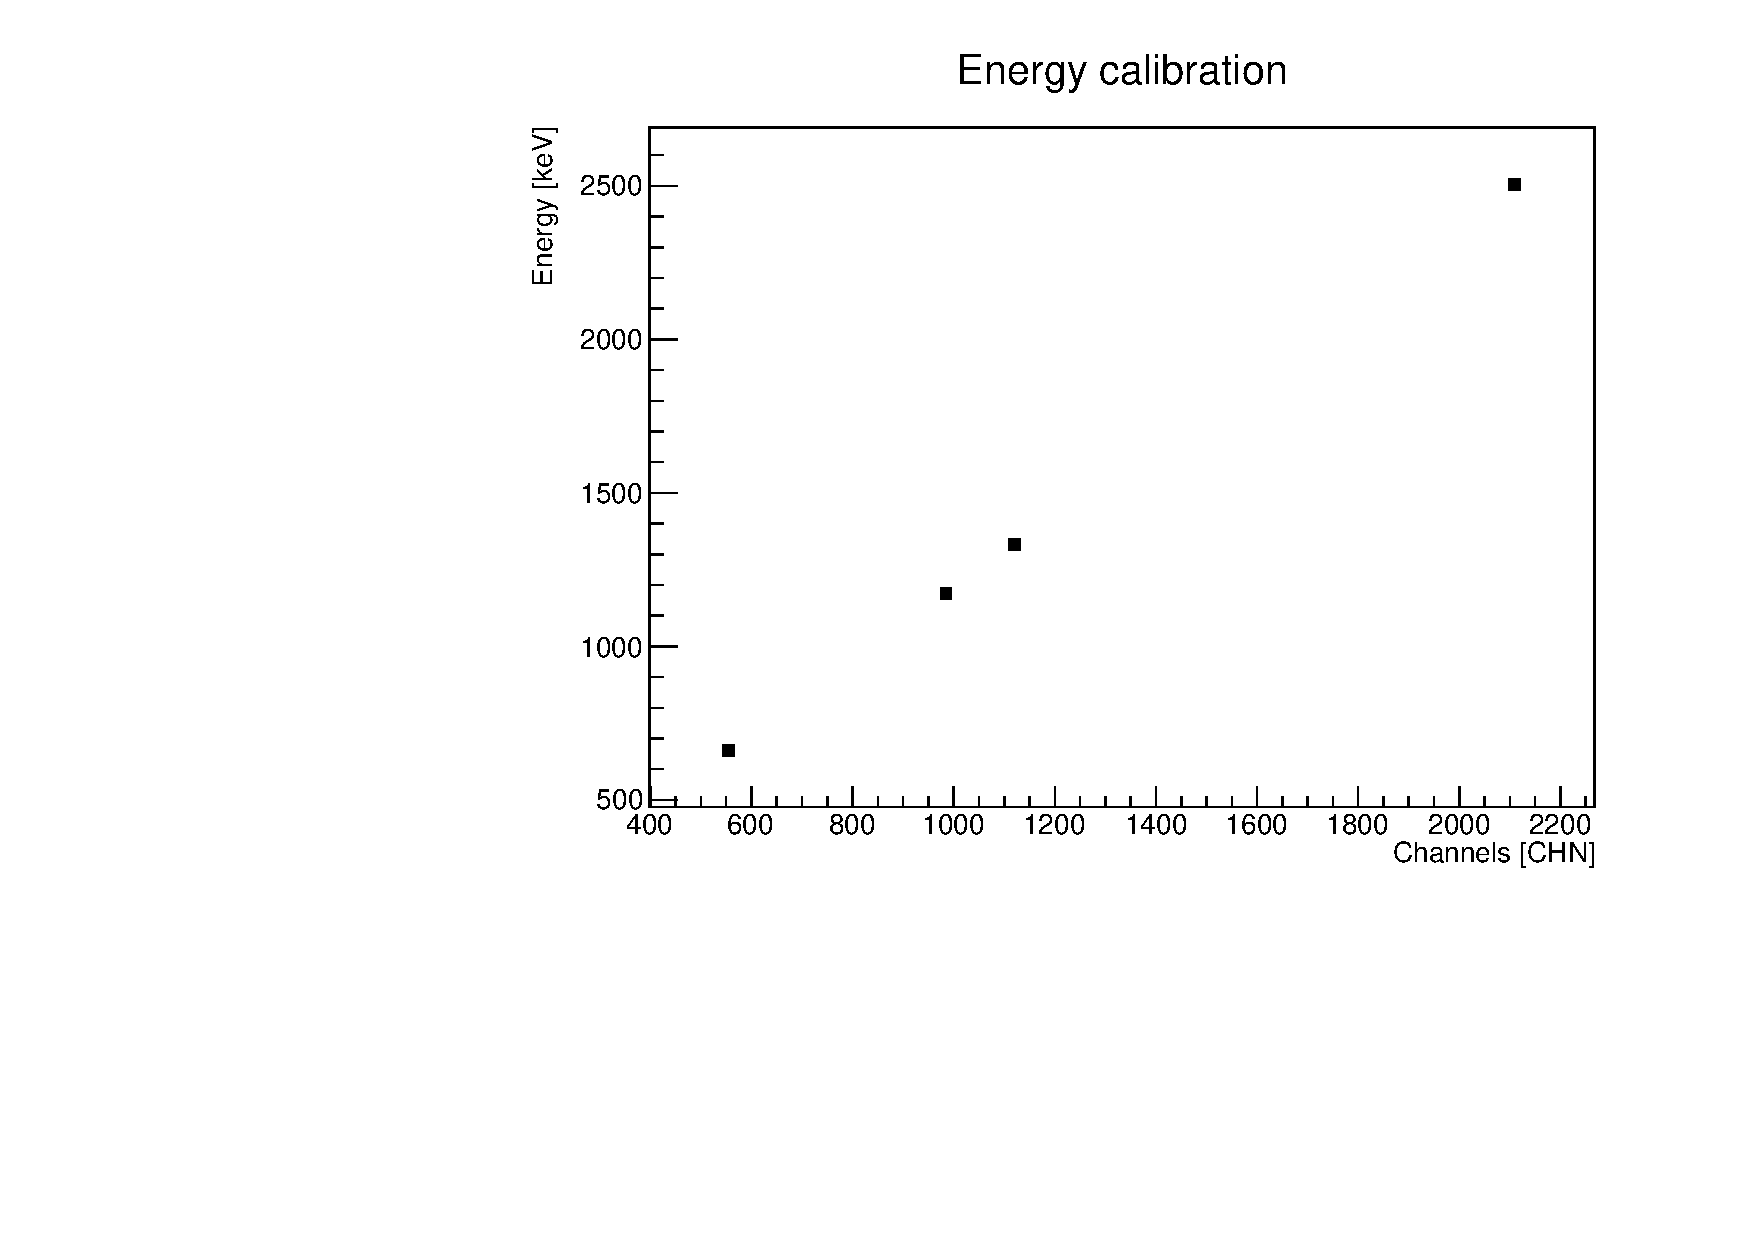
\includegraphics[width=0.9\textwidth]{img/plot0_empty.pdf}}
				\uncover<3->{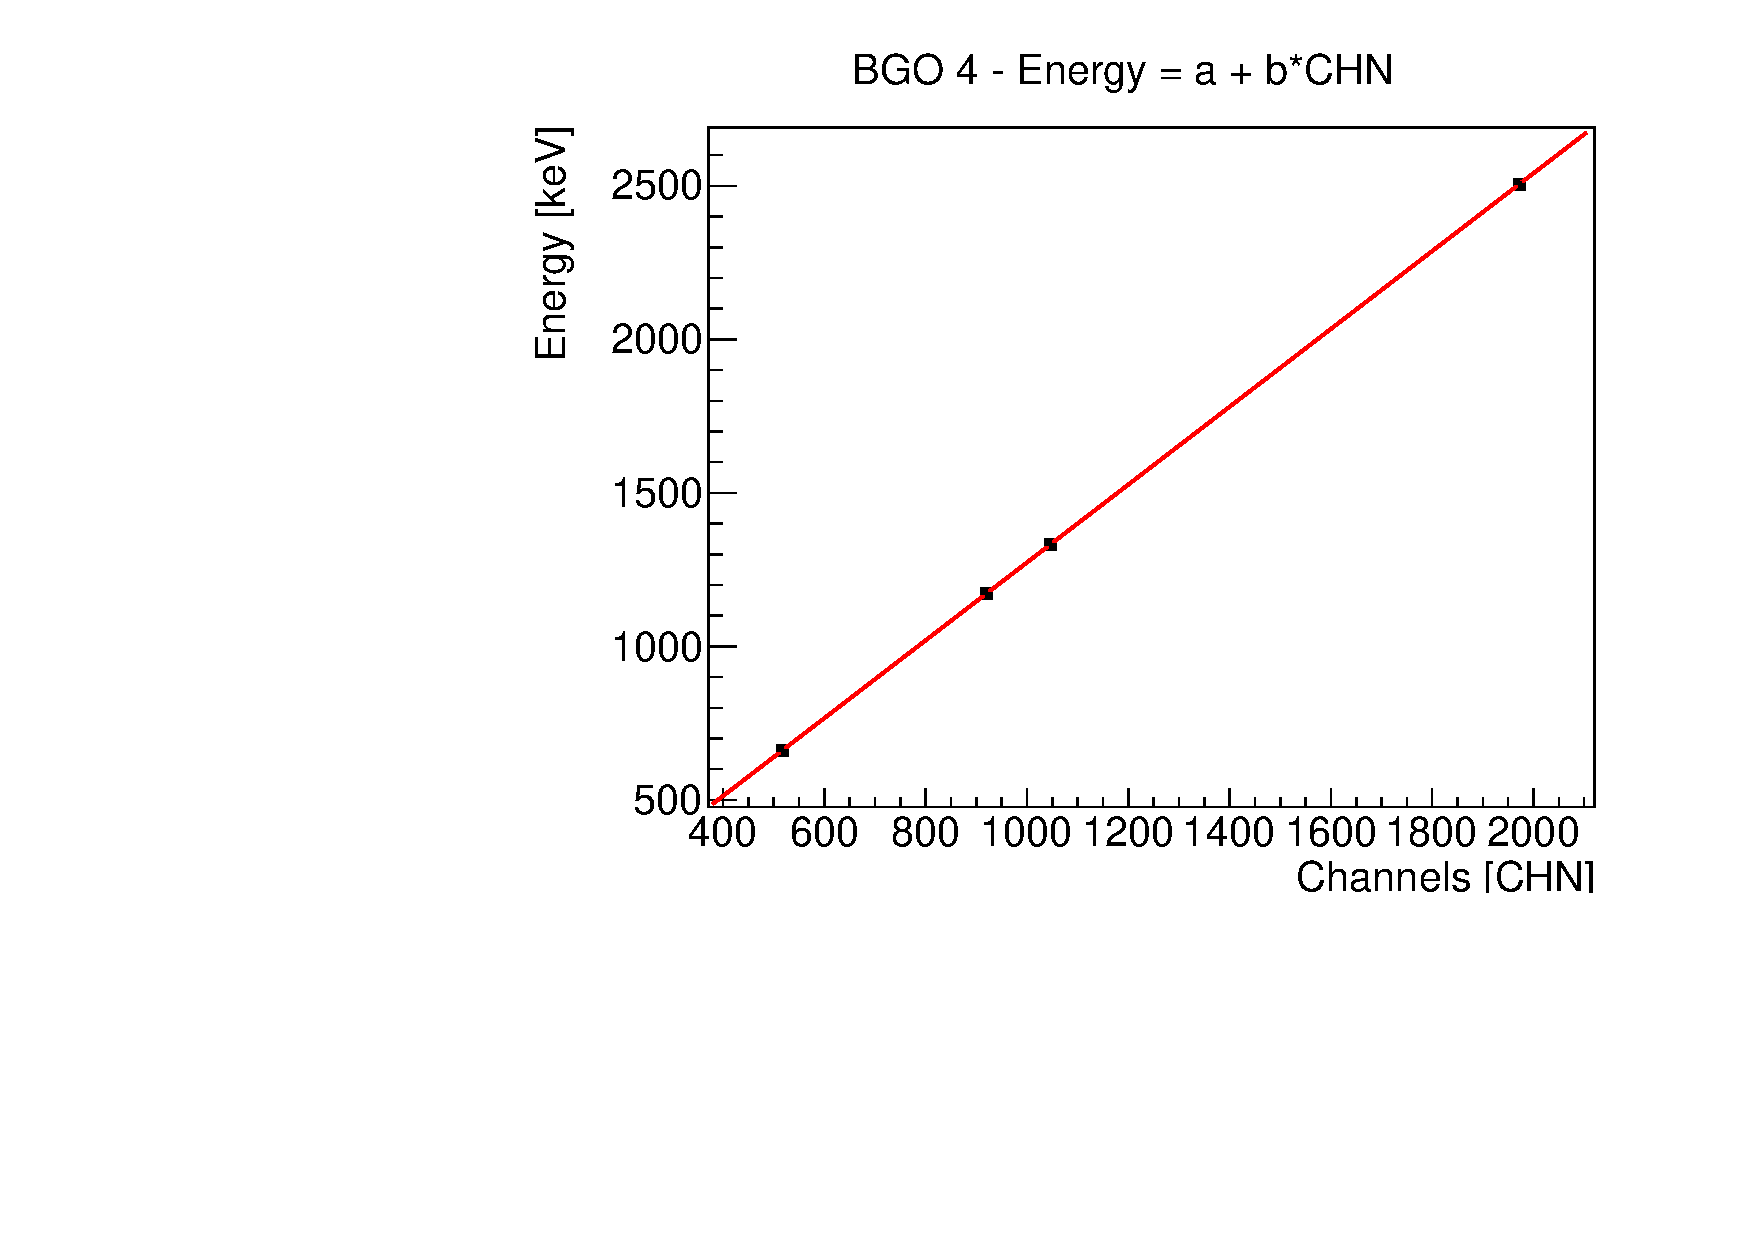
\includegraphics[width=0.9\textwidth]{img/plot0.pdf}}
				\uncover<5->{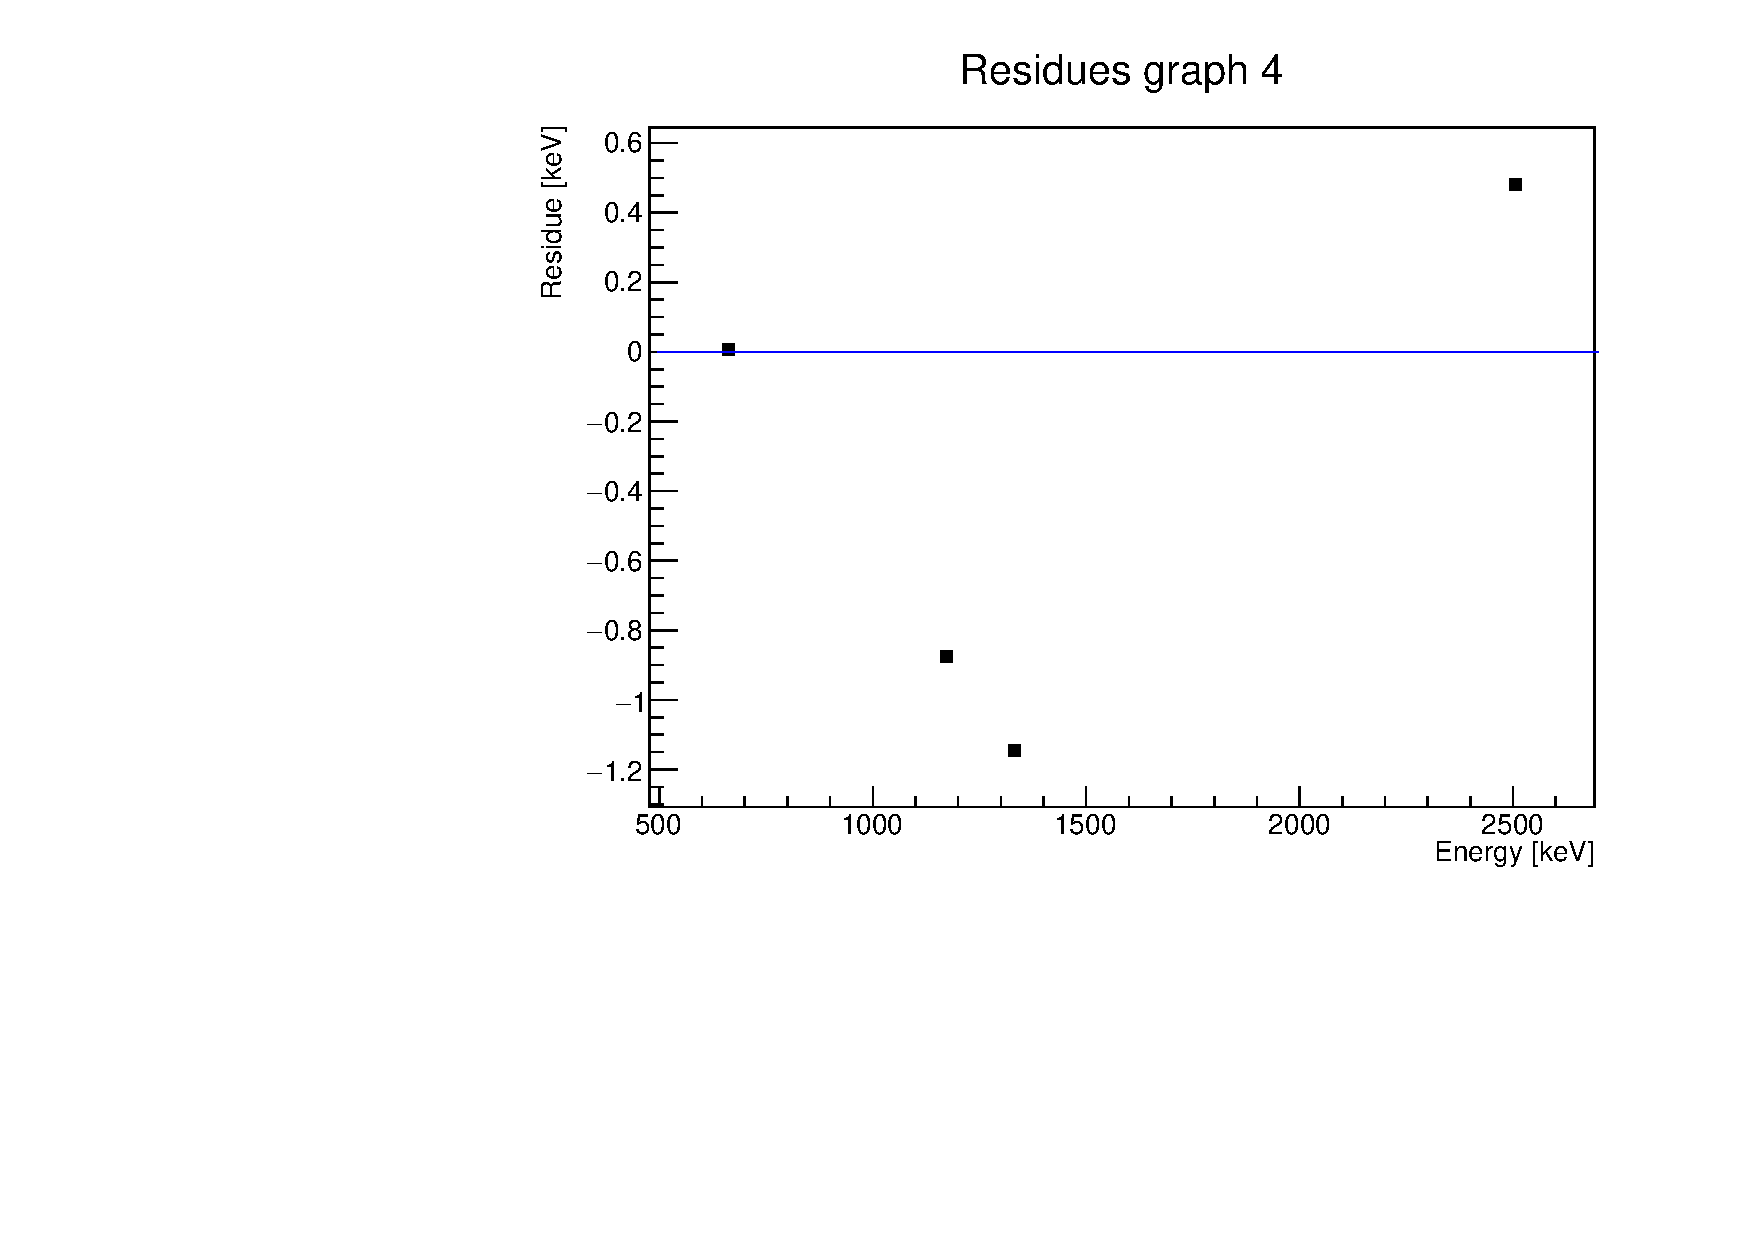
\includegraphics[width=0.9\textwidth]{img/residues0.pdf}}
%				\only<4->{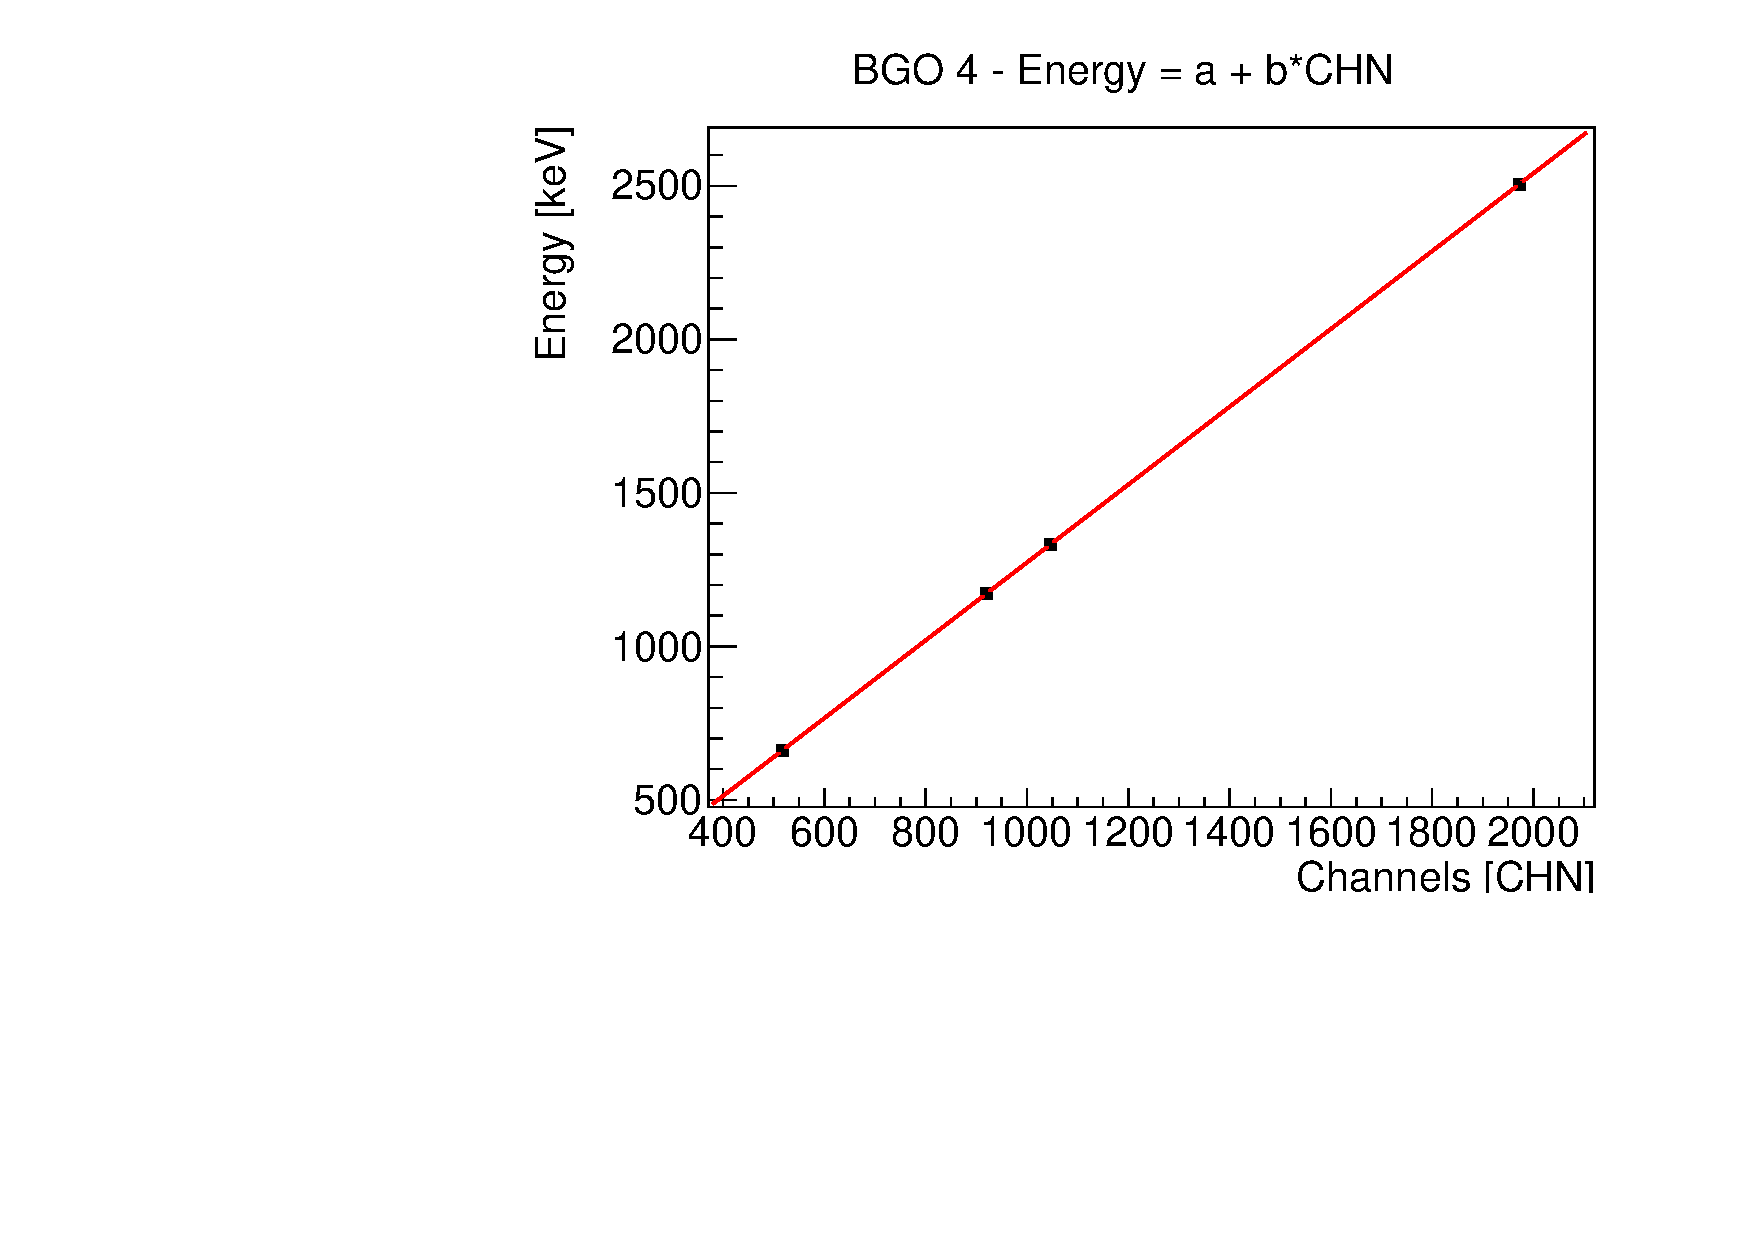
\includegraphics[width=0.9\textwidth]{img/plot0.pdf}}
				%TERZA GRAFICA PER FARE VEDERE I RISULTATI
			%chiamare conversione b e agiugngere a
		
		\end{column}
	\end{columns}
	%grafico lineare, valori parametri in un angolo della slide
	%retta per il quarto spicchio, spettro del quarto, tabella (possibilmente quarto spicchio)
	%mettere espressione
	%mettere residui
\end{frame}%mettere energy =

\section{Efficienza}
\begin{frame}{Efficienza}
	\begin{itemize}
		\item<1-> L'efficienza è un fattore fondamentale per ricavare la sezione d'urto.
		\item<2-> Si può calcolare dall'espressione:
		\begin{equation}
			\varepsilon = \dfrac{N_{cont.}}{A(t*) \Delta t}
		\end{equation}
		\item<3-> L'attività è calcolata al momento della misurazione (sorgenti radioattive di attività nota con precisione del 0.5\%) %verificare).
	\end{itemize}
	
	\vspace{0.5cm}
	
	% This part will be revealed on the second slide (within the same frame)
		\begin{columns}
			\begin{column}{0.5\textwidth}
				\visible<4->{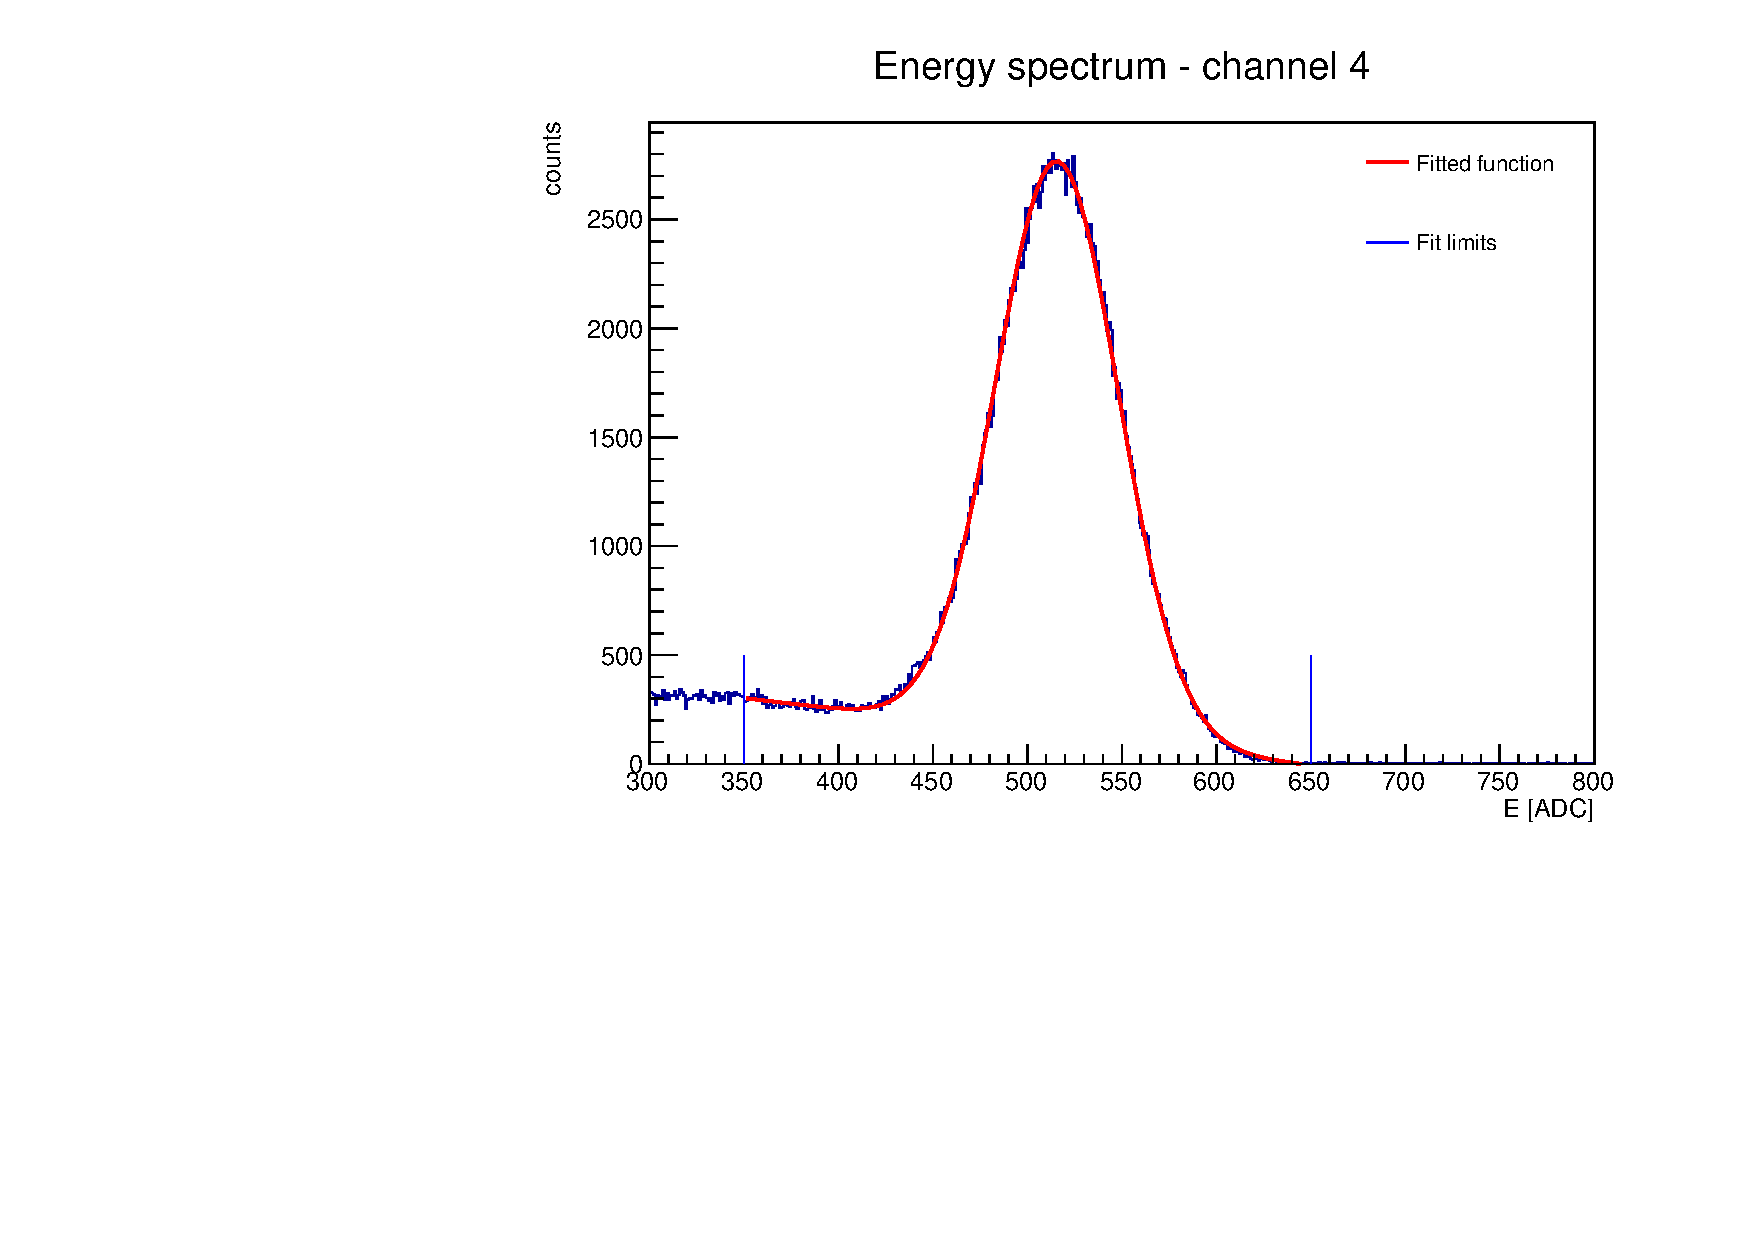
\includegraphics[width=\textwidth]{img/parameter.pdf}}
			\end{column}
			\begin{column}{0.5\textwidth}
				\visible<5->{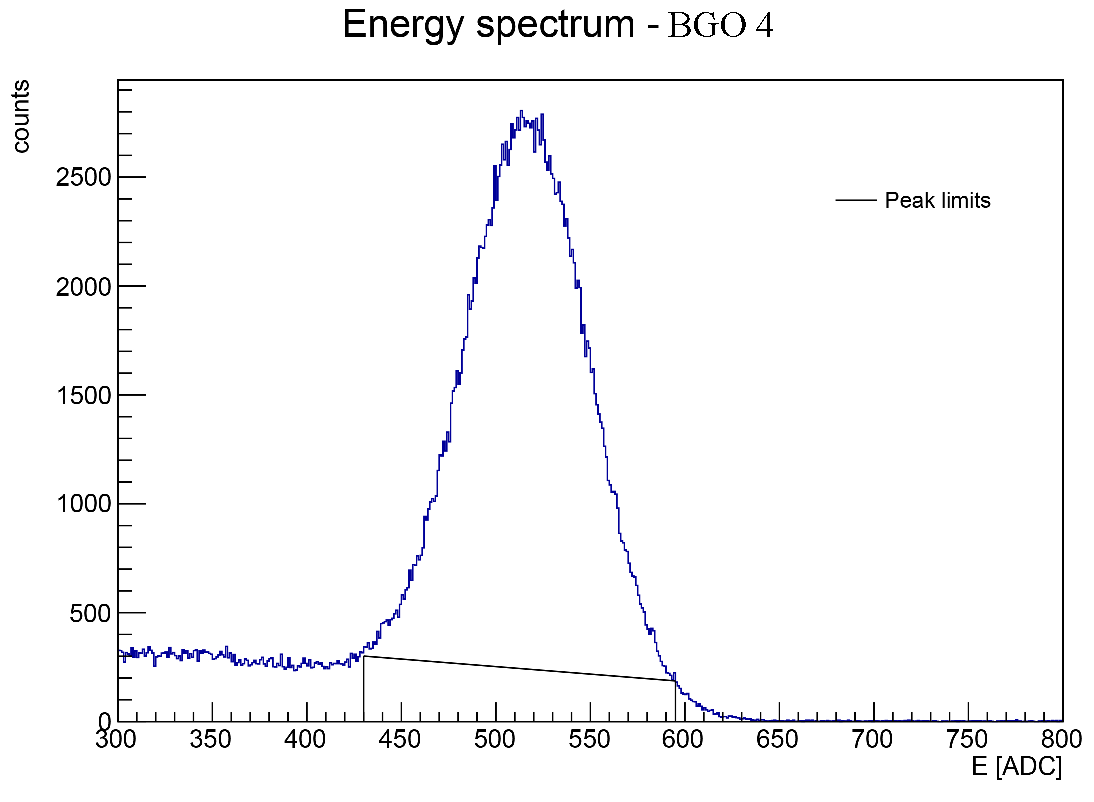
\includegraphics[width=\textwidth]{img/trapezoid.pdf}}
			\end{column}
		\end{columns}
\end{frame}

%\begin{frame}{Calcolo dell'efficienza}%si può dire tutto a voce, sulla immagine del picco senza fit (dall'altra parte mettere immagine con fit)
%	\begin{itemize}
%		\item Per il calcolo dell'efficienza è necessario trovare il numero di conteggi nei picchi gaussiani. Si possono applicare due metodi diversi per trovarlo:
%	\end{itemize}
%	\hrule height 0.3mm \vspace{2mm}
%	
%	\begin{columns}
%		\column{0.5\textwidth}
%		\uncover<2->{\centering \emph{Trapezio} 
%			\begin{itemize}
%				\item Metodo geometrico
%				\item Consiste nell'isolare la regione del picco e rimuoverne il fondo trapezoidale
%				\item Adatto solo per il cesio: i due picchi del cobalto non sono sufficientemente risolti dallo strumento
%		\end{itemize}}
%		
%		\column{0.5\textwidth}
%		\uncover<3->{\centering \emph{Parametrico}
%			\begin{itemize}
%				\item Metodo che sfrutta i parametri del fit
%				\item Il coefficiente di normalizzazione del picco gaussiano è il numero di conteggi nel picco
%				\item Adatto per cesio e cobalto
%		\end{itemize}}
%	\end{columns}
%	
%\end{frame}

\begin{frame}{Tempo morto}%solo tempo vivo, indicare per spicchio 4 quanto vale. (tempo morto anziché tempo vivo)
	\begin{itemize}
		%\item L'attività viene calcolata al momento della presa dati, in data 03/04/2024
		\item<1-> Il pulser serve per stimare il tempo morto dell'elettronica
		%rimettere schema elettronica
		\item<2-> Questo, a frequenza nota, è mandato in ogni spicchio del BGO e si confronta con la frequenza misurata in ogni rivelatore
		\item<3-> Per lo spicchio 4 il tempo morto è circa l'$\mathbf{1.3\%}$ 
	\end{itemize}
	%leva gli istogrammi
	%mettere schema elettroncia
	\uncover<2->{\centering
		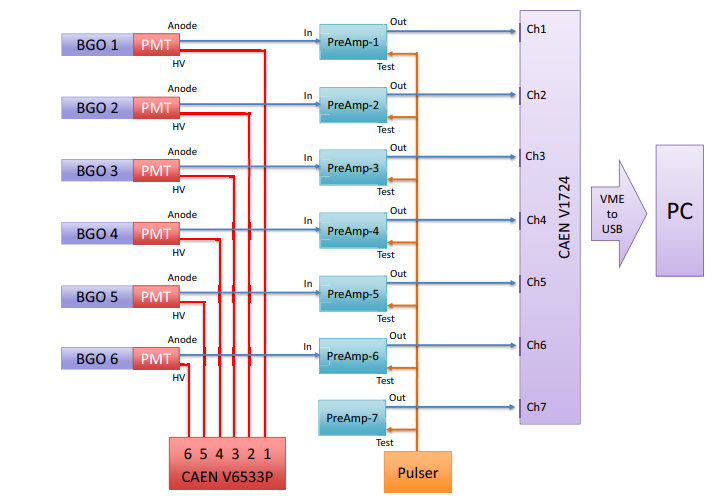
\includegraphics[width=0.6\textwidth]{img/electronics.png}}
\end{frame}











\section{Simulazioni}

\begin{frame}{Simulazioni}
	\begin{itemize}
		\item<1-> Il setup sperimentale e la reazione $^{14}$N(p,$\gamma$)$^{15}$O sono stati simulati in GEANT4
		\item<2-> Gli spettri ottenuti con queste simulazioni sono a risoluzione energetica infinita
		\item<3-> Questi sono stati analizzati applicando la risoluzione energetica degli spettri sperimentali
	\end{itemize}
\end{frame}

\begin{frame}{Risoluzione energetica}%inserire spettro simulato con ris inf e far veder come viene fuori con risoluzione dopo applicazione
%	\begin{itemize}
%		\item Le simulazioni contengono picchi di energia ideali, a cui non è stata applicata la risoluzione dello strumento
%		\item Questa si può trovare eseguendo fit gaussiani sugli istogrammi in energia, anziché canali
%		\item La risoluzione è il rapporto tra la deviazione standard del picco e la corrispondente energia nota
%		\item Le risoluzioni si mettono su un grafico contro le corrispettive energie note, fittandovi una funzione:
%		
%		\begin{equation*}
%			f(E) = a + \dfrac{b}{\sqrt{E}}
%		\end{equation*}
%	\end{itemize}
%lasciare funzione fittata

	\begin{columns}
		\begin{column}{0.5\textwidth}
			\only<1->{\centering
				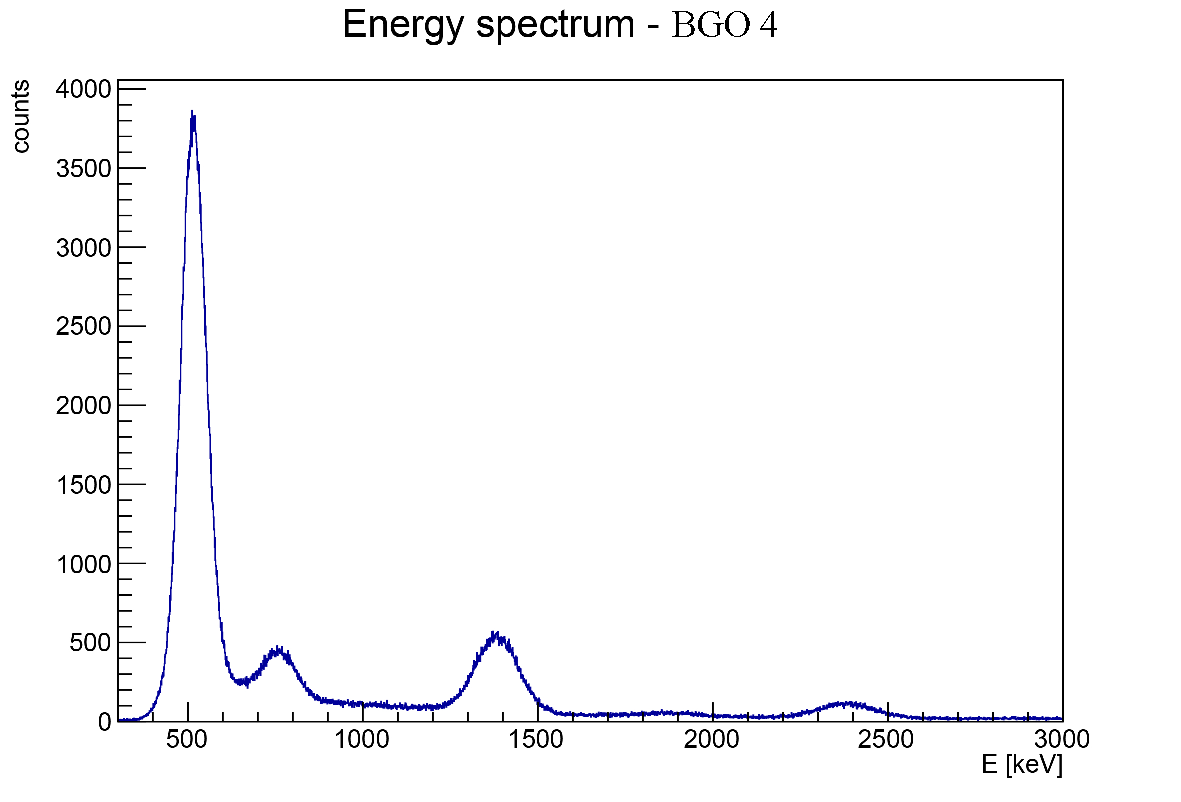
\includegraphics[width=0.9\textwidth]{img/resolution_hist1.pdf}
				\centering
				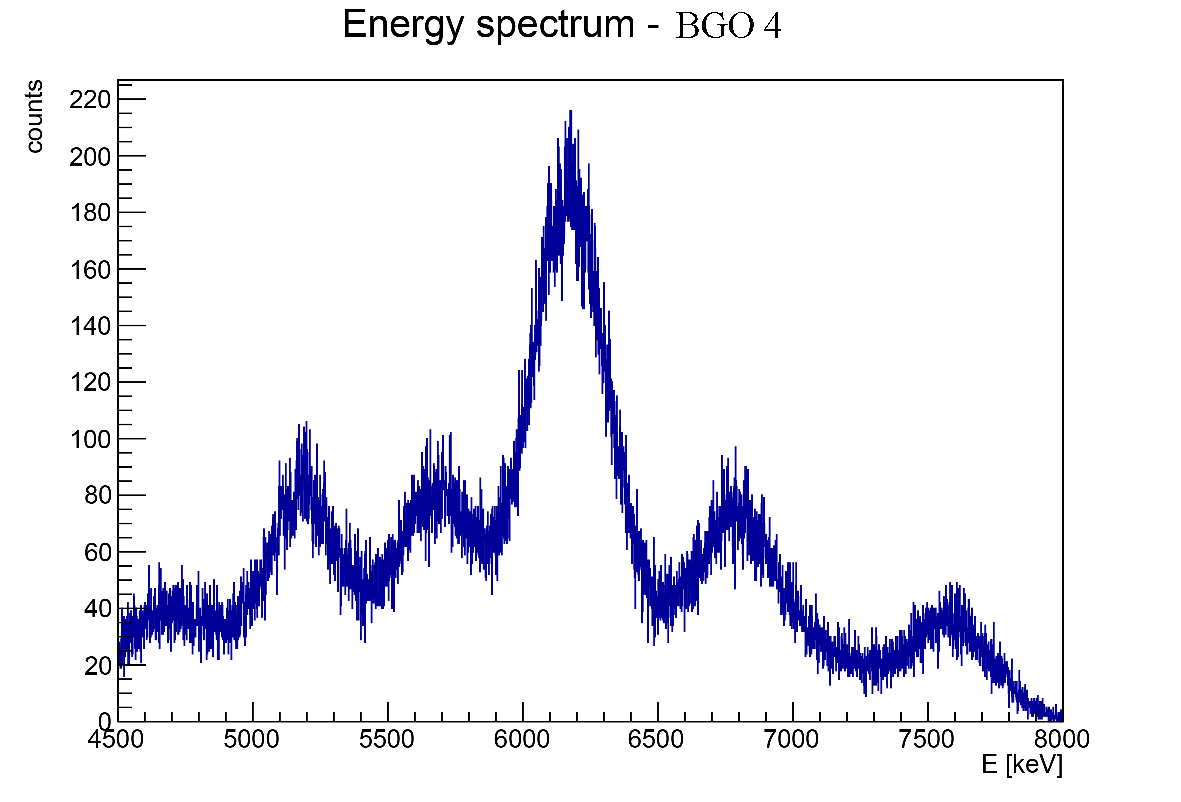
\includegraphics[width=0.9\textwidth]{img/resolution_hist2.pdf}}
		\end{column}
		\begin{column}{0.5\textwidth}
			\visible<2->{\begin{itemize}
					\item Per trovare la risoluzione energetica si fitta la funzione:
				\end{itemize}
				\begin{equation*}
					f(E) = a + \dfrac{b}{\sqrt{E}}
			\end{equation*}}	
			\visible<3->{\centering
				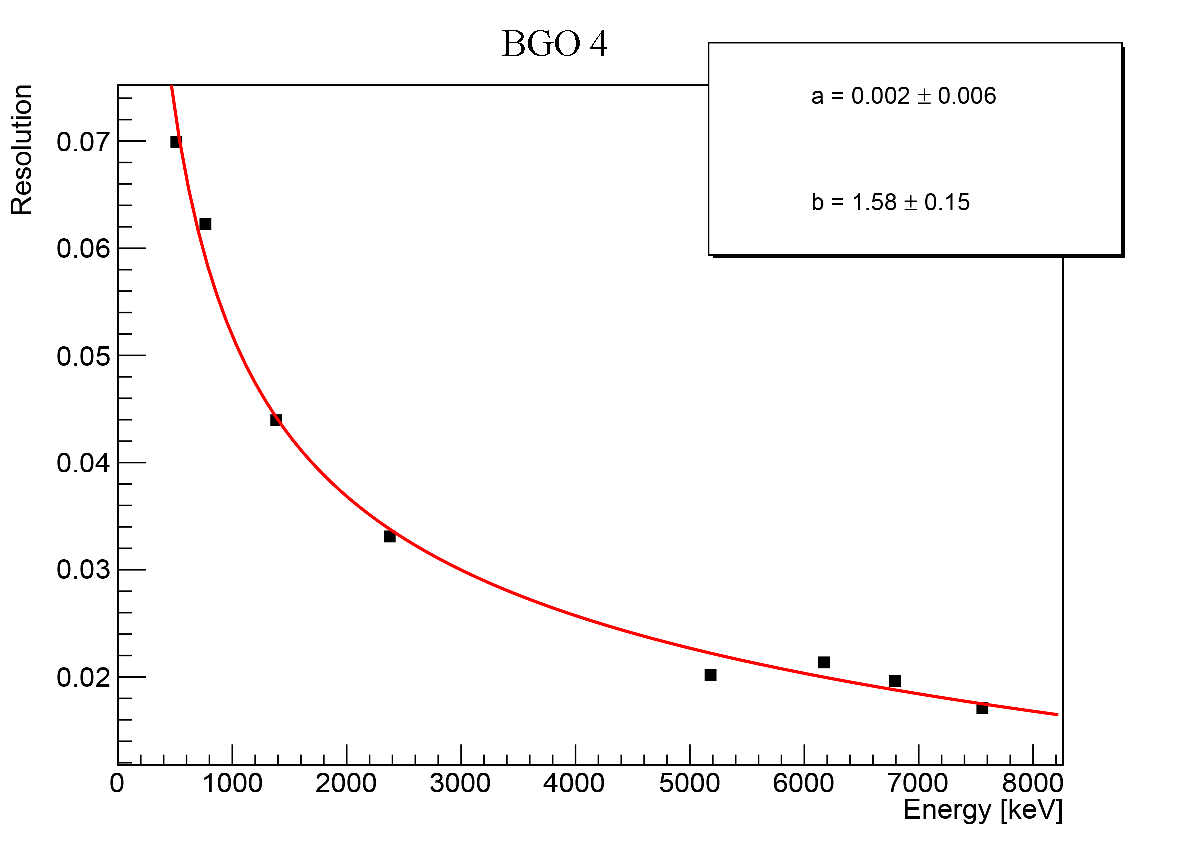
\includegraphics[width=0.9\textwidth]{img/ResGraph_4.pdf}}
		\end{column}
	\end{columns}
\end{frame}

\begin{frame}{Simulazioni}%mettere confronti uno di fianco all'altro, ingrandire tabella
	\begin{columns}
		\begin{column}{0.45\textwidth}
			\uncover<1->{\centering
			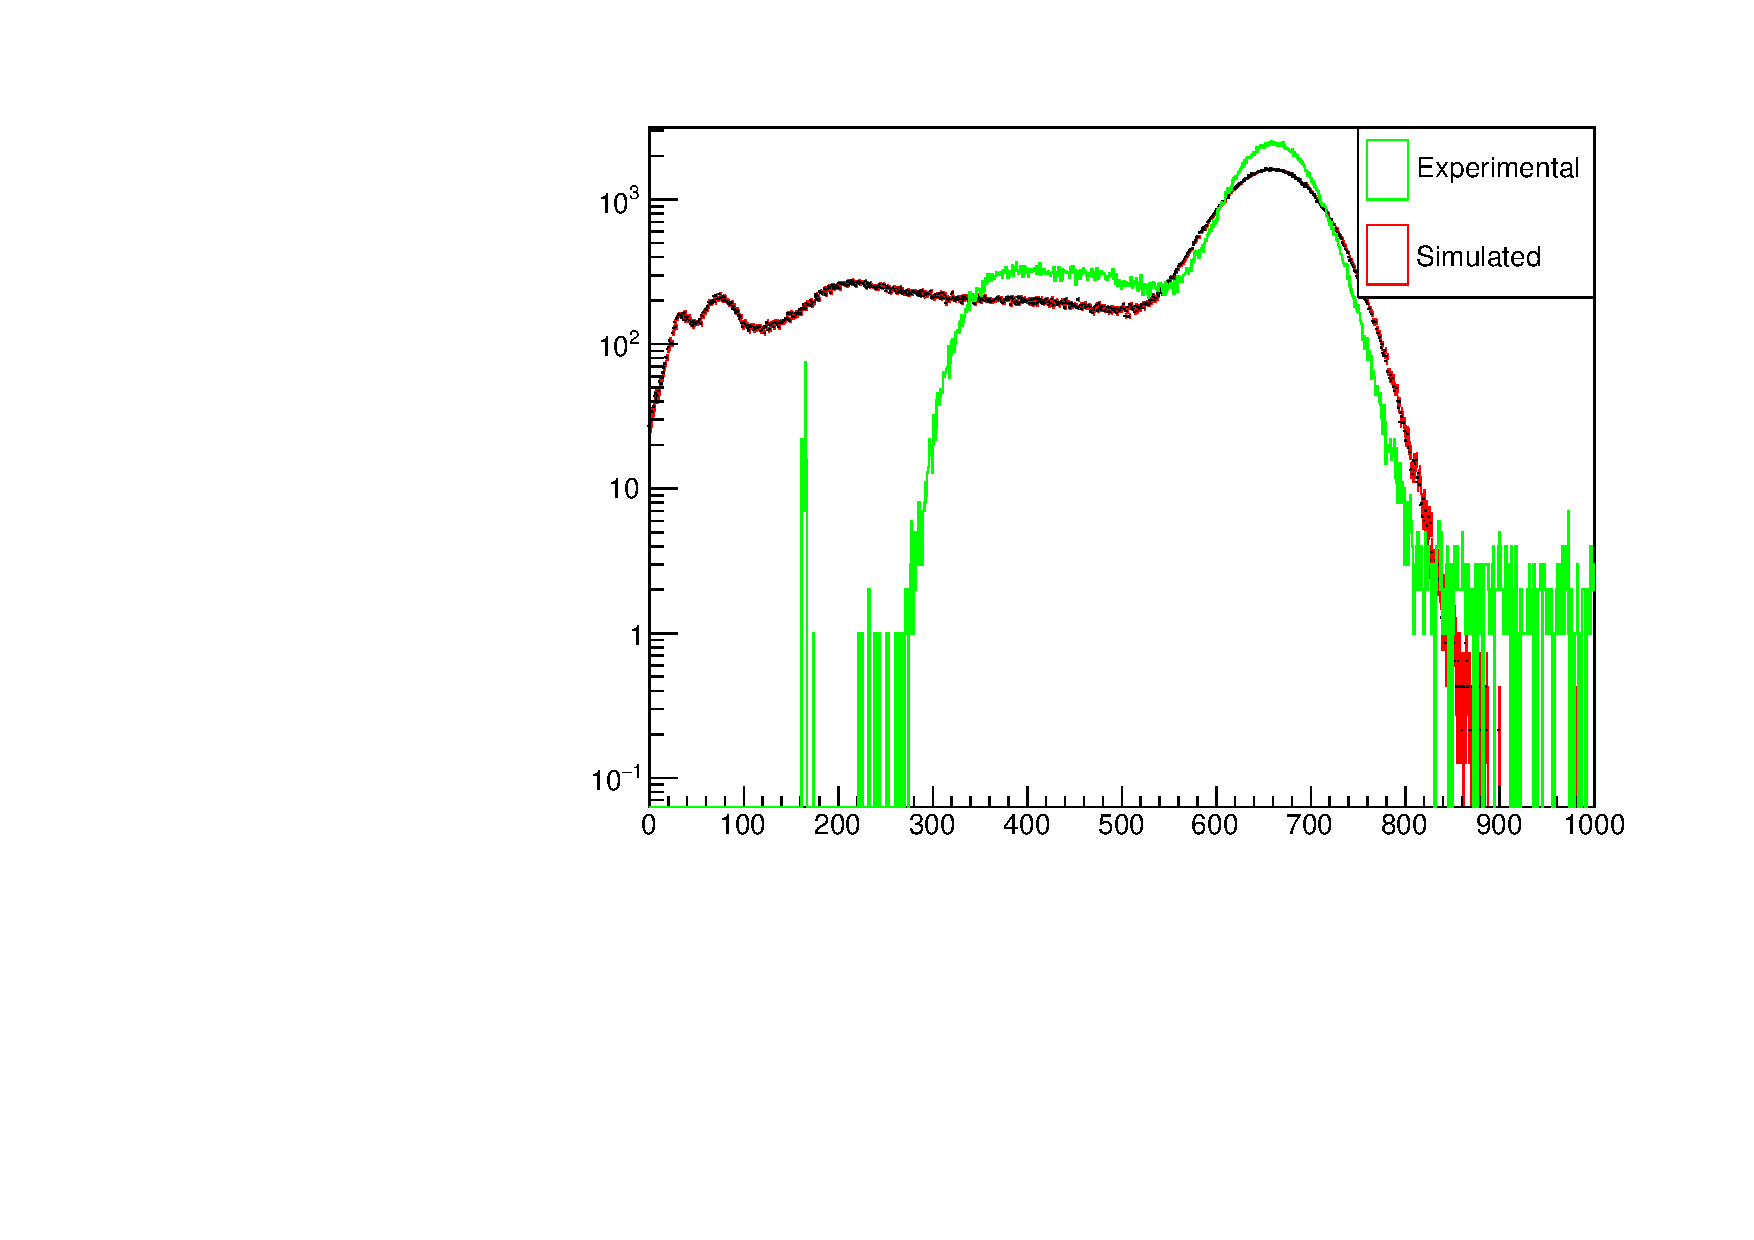
\includegraphics[width=\textwidth]{img/Caesium.pdf}}
			
		\end{column}
	\begin{column}{0.45\textwidth}
%		\only<1->{\centering
%		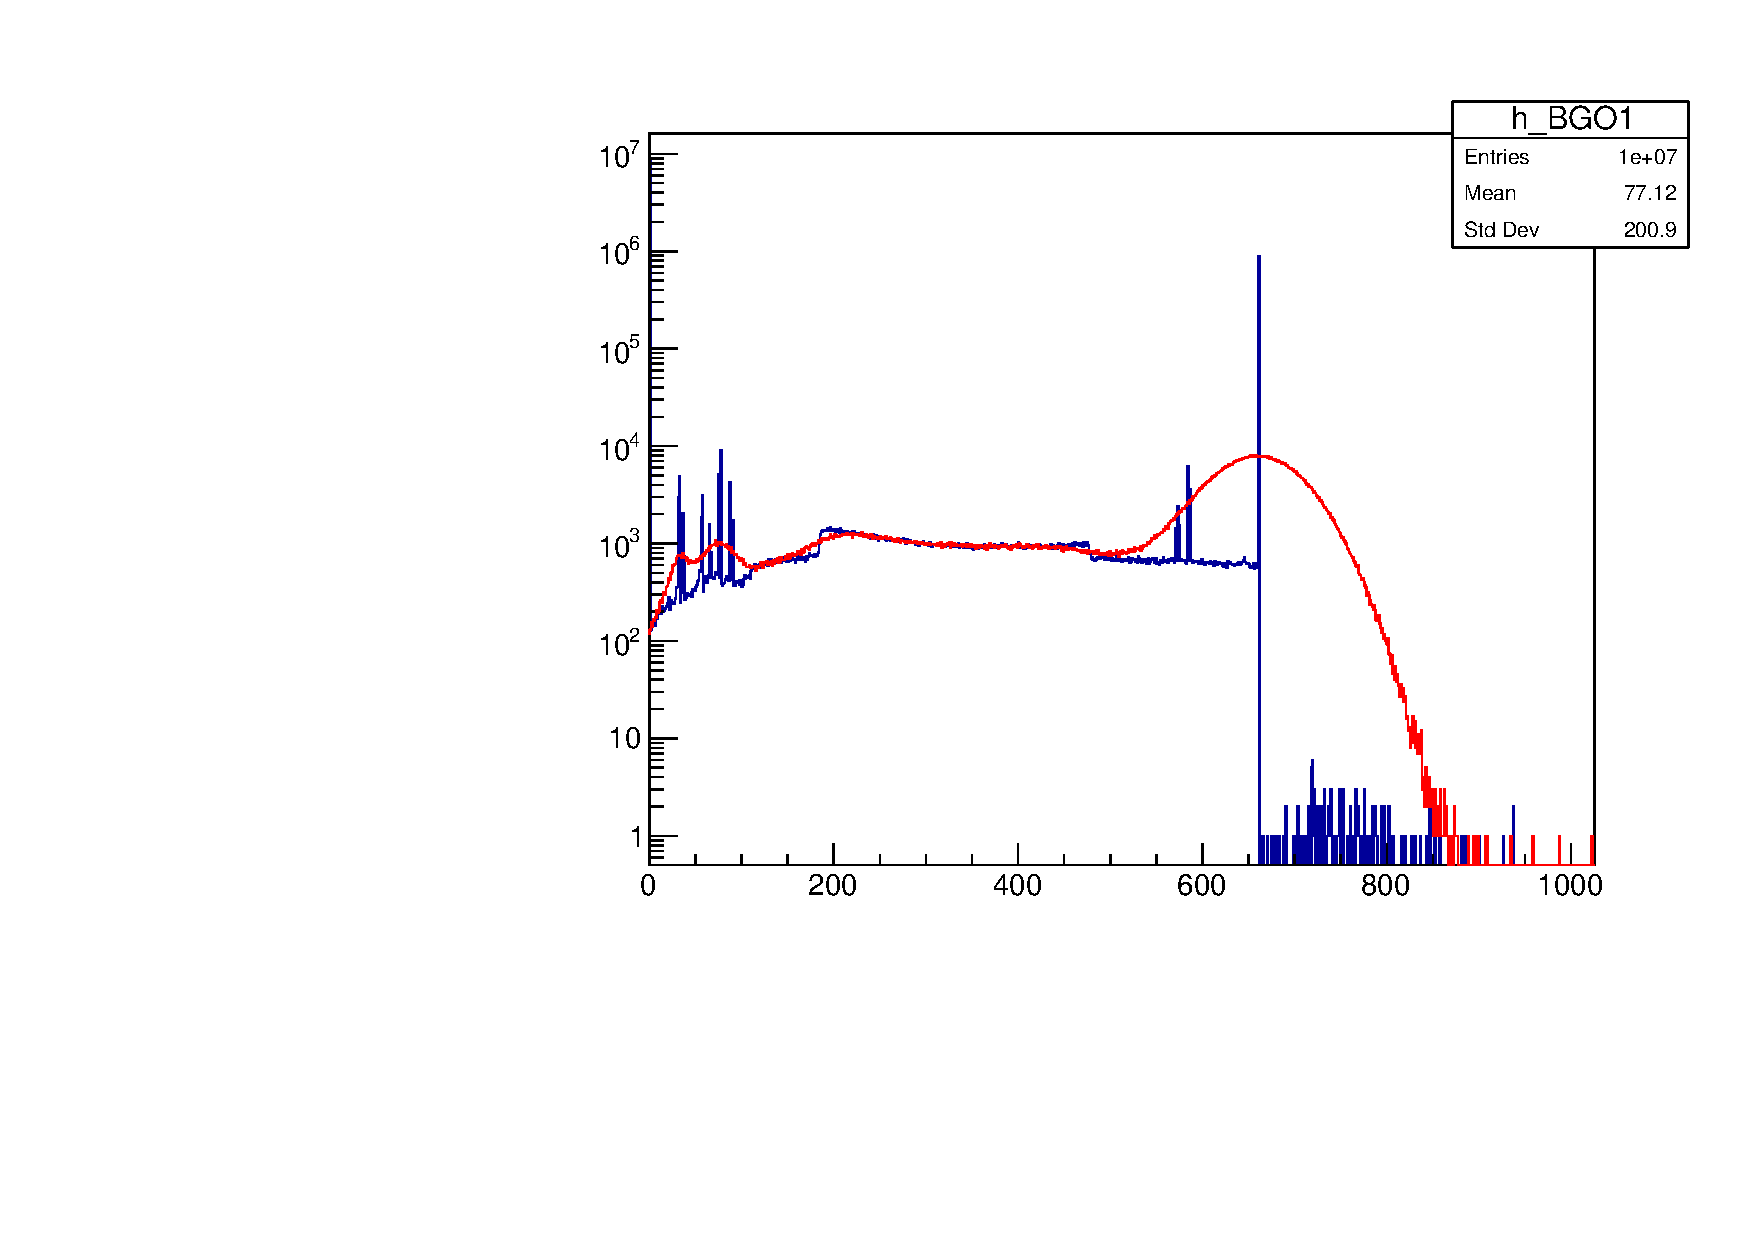
\includegraphics[width=\textwidth]{img/nonscaled.pdf}}
		\uncover<2->{\centering
			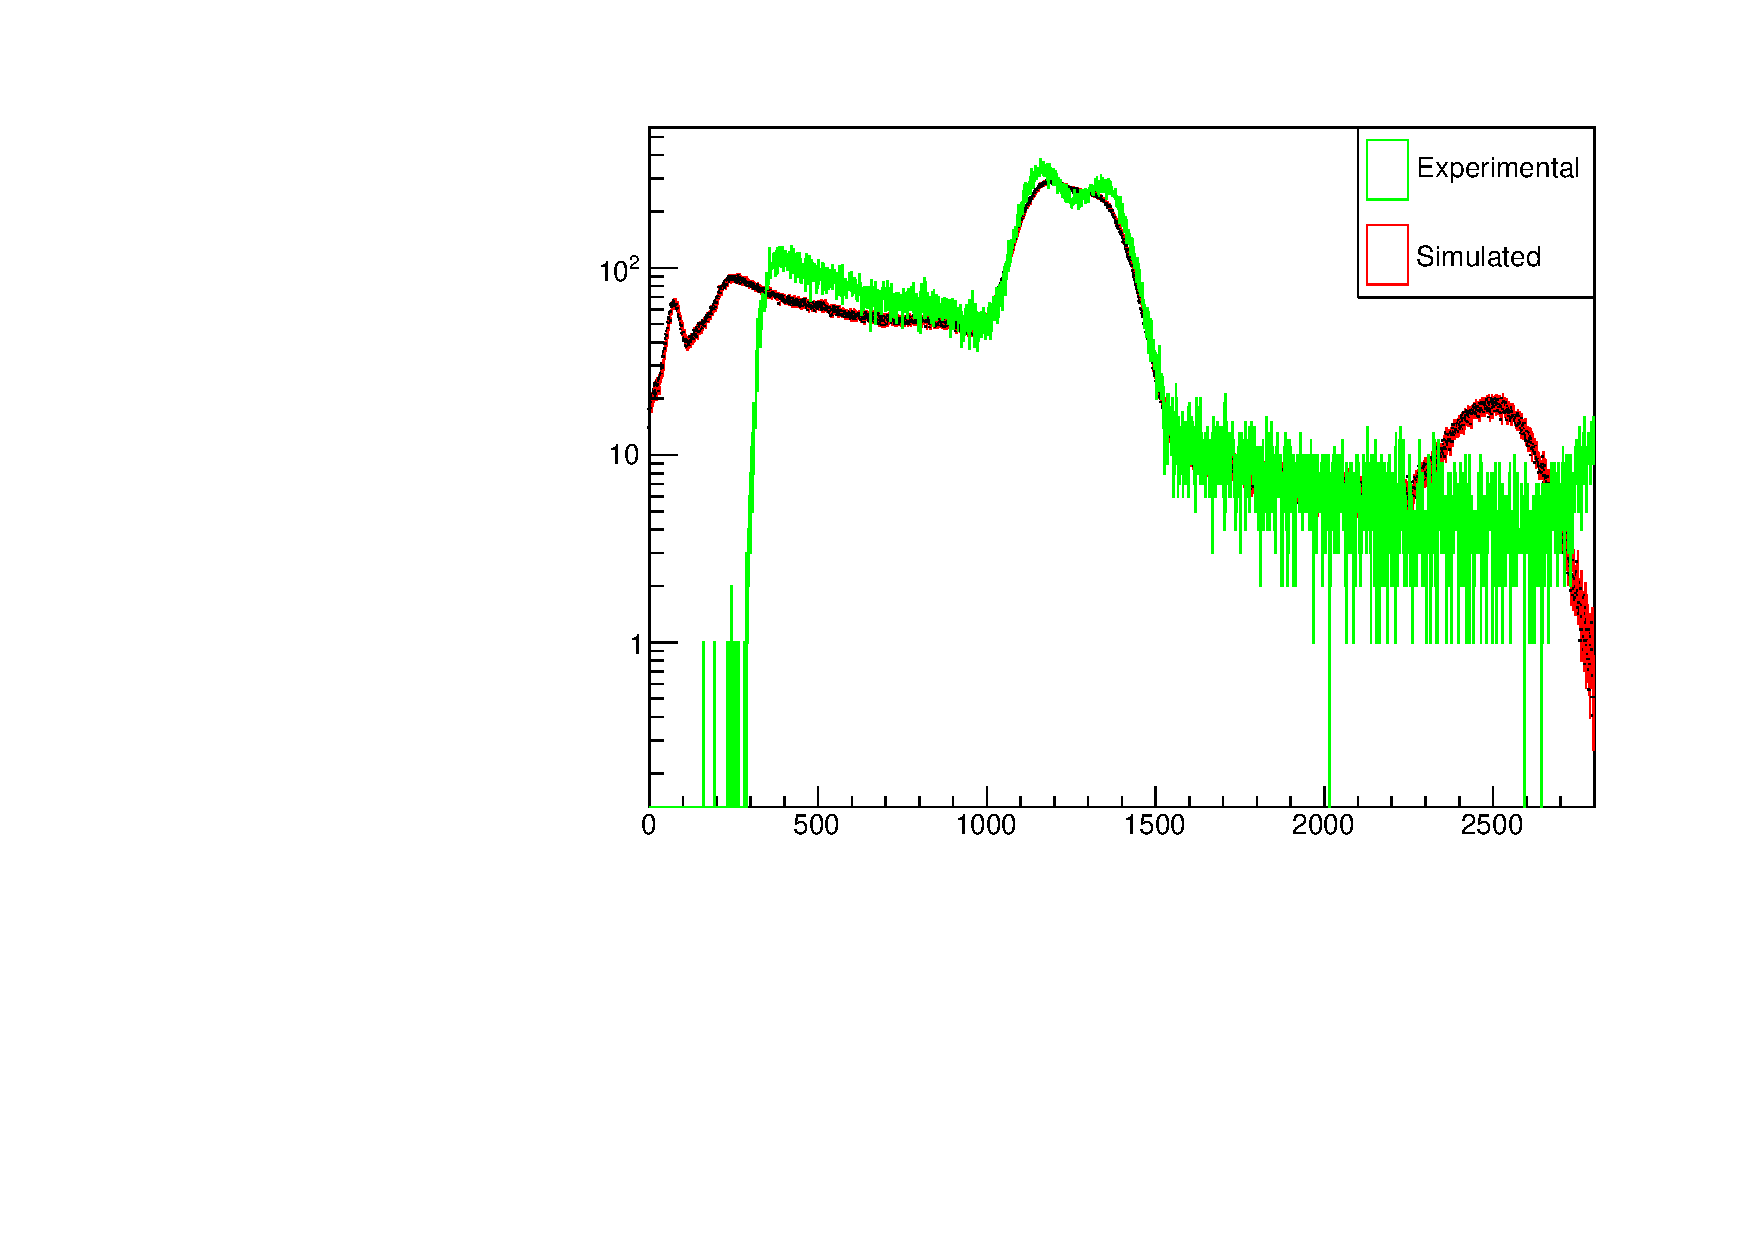
\includegraphics[width=\textwidth]{img/Cobalt.pdf}}
	\end{column}%errore di tutte le efficienze del 5%
	\end{columns}
\uncover<3->{\begin{table}[h]
		\centering
		
		\resizebox{0.9\textwidth}{!}{
			\begin{tabular}{@{}cccc@{}}
				\toprule
				CHN4 & Efficienza \% (sim.) & Efficienza \% (exp.) \\ \midrule
				$^{137}$Cs (661 keV) & 10.8 \(\pm\) 0.5 & 10.2 \(\pm\) 0.5 \\
				$^{60}$Co (1173 keV) & 7.9 \(\pm\) 0.4 & 8.1 \(\pm\) 0.4 \\
				$^{60}$Co (1332 keV) & 7.8 \(\pm\) 0.4 & 7.5 \(\pm\) 0.4 \\
				\bottomrule
		\end{tabular}}
\end{table}}%mettere in percentuale
\end{frame}
	
	\section{Conclusione}
	\begin{frame}{Conclusione}
		\begin{itemize}
			\item<1-> Durante la tesi ci si è occupato della calibrazione di uno strumento per lo studio della reazione  $^{14}$N(p, $\gamma$)$^{15}$O
			\item<2-> Il rivelatore utilizzato è stato calibrato in energia e ne si è calcolata l'efficienza
			\item<3-> Si sono analizzate le simulazioni Monte Carlo, per poi confrontarle coi dati sperimentali
		\end{itemize}
	\end{frame}
	
	\begin{frame}{Fine}
		\centering
		\textbf{Grazie per l'attenzione.}
	\end{frame}
	
\begin{frame}{Backup}
	\centering
	Slide di backup
\end{frame}
	
\begin{frame}{L'esperimento}
	\begin{itemize}
		\item<1-> L'esperimento LUNA (Laboratory for Underground Nuclear Astrophysics) ricrea i processi nucleari che sono avvenuti durante la nucleosintesi primordiale e che avvengono tutt'ora nelle stelle.
		\item<2-> Essendo processi molto rari, un laboratorio sulla superficie terrestre non è adatto per le misure sperimentali di questi, poiché i raggi cosmici maschererebbero il segnale debole atteso.
	\end{itemize}
\end{frame}


\begin{frame}{Motivazione astrofisica}
	\begin{itemize}
		\item<1-> I neutrini solari giocano un ruolo fondamentale nella determinazione della composizione del Sole.
		\item<2-> Sono prodotti nel ciclo CNO del Sole.
		\item<3-> In particolare, la sezione d'urto della reazione $^{14}$N(p, $\gamma$)$^{15}$O è la fonte di errore principale sulle stime del flusso di neutrini, in quanto la più breve dell'intero ciclo.
		\item<4-> A energie solari (15-50 keV) la sezione d'urto è troppo piccola per essere misurata direttamente.
		\item<5-> La tesi ha come obiettivo contribuire alla determinazione della sezione d'urto ad energie 50-370 keV.
	\end{itemize}
\end{frame}
\begin{frame}{Proposta dell'esperimento}
	\begin{itemize}
		\item<1-> A energie solari (15-50 keV) la sezione d'urto è troppo piccola per essere misurata direttamente.
		\item<2-> Le stime odierne sono quindi estrapolazioni da energie più alte.
		\item<3-> Il progetto ha come obiettivo determinare la sezione d'urto ad energie 50-370 keV.
	\end{itemize}
\end{frame}

\begin{frame}{Reaction rate}
	\begin{itemize}
			\item<1-> Il \emph{reaction rate} ($N_{reaz}/\Delta t$) vale quindi appena $1\div 10$ conteggi al giorno
			\item<2-> Basta pochissimo rumore per nascondere i segnali che rivelano le reazioni
			\item<3-> La soluzione è cercare di minimizzare il rumore di fondo 
		\end{itemize}
\end{frame}

	\begin{frame}{Località}
			\begin{columns}
					\begin{column}{0.5\textwidth}
							\begin{itemize}
									\item<1-> I Laboratori Nazionali del Gran Sasso, situati nella frazione di Assergi, sono schermati dai 1400 m di roccia del Monte Aquila.
									\item<2-> Ciò fa sì che il fondo di raggi cosmici sia fortemente soppresso
									\item<3-> Qui è collocato l'acceleratore LUNA2 a 400 kV, che permette di concentrare fasci ionici molto intensi e stabili.
								\end{itemize}
						\end{column}
					\begin{column}{0.5\textwidth}
			tenere immagine
							\centering
							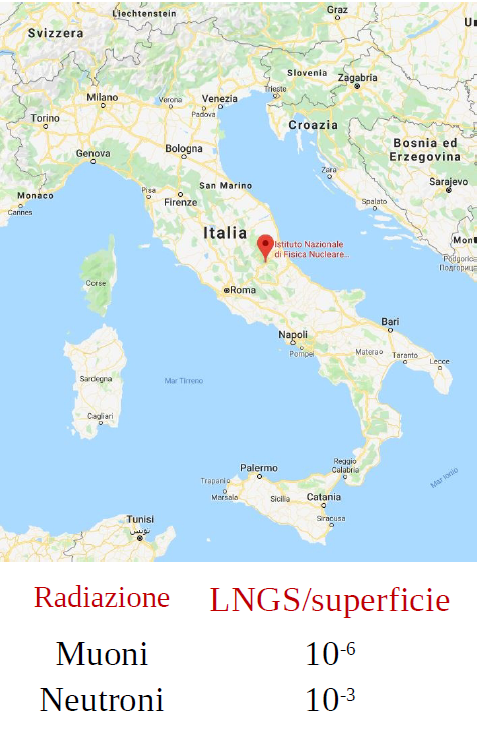
\includegraphics[width=0.8\textwidth]{img/location.png}
							\captionof{figure}{LNGS, Assergi, AQ.}
						\end{column}
				\end{columns}
		\end{frame}

	\begin{frame}{Il rivelatore $4\pi$}
	\begin{columns}
		\begin{column}{0.45\textwidth}
			\begin{itemize}
				%\item La radiazione gamma emessa dalla reazione è rivelata da uno scintillatore.
				\item Si tratta di un rivelatore in germanato di bismuto (Bi$_{4}$Ge$_{3}$O$_{12}$, detto BGO), coprente il 95\% dell'angolo solido totale attorno al bersaglio.
				\item Si tratta di uno scintillatore, ossia uno strumento che quando eccitato da radiazione ionizzante, ne assorbe l'energia depositata e la riemette sotto forma di fotoni
			\end{itemize}
		\end{column}
		\begin{column}{0.45\textwidth}
			\centering
			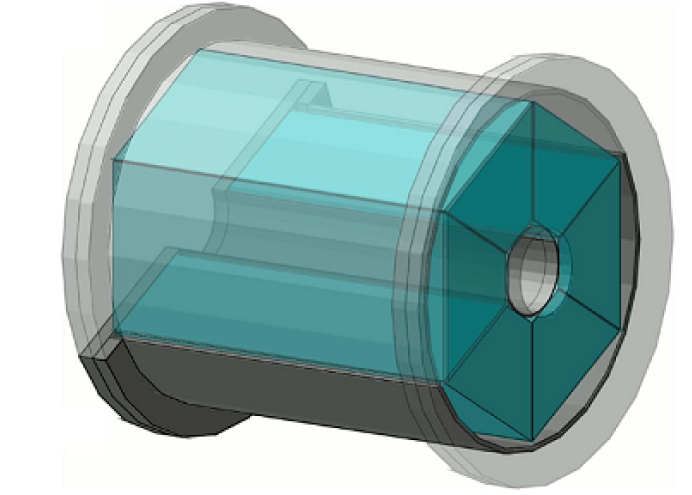
\includegraphics[width=\textwidth]{img/bgo_3d.png}
			\captionof{figure}{Rappresentazione 3D del rivelatore BGO.}
		\end{column}
	\end{columns}
	
\end{frame}

\begin{frame}{Il rivelatore $4\pi$}
	\begin{columns}
		\begin{column}{0.45\textwidth}
			\begin{itemize}%a voce
				\item Il cristallo, a simmetria cilindrica, è otticamente separato in 6 spicchi uguali.
				%\item I fotoni di scintillazione di ciascuno dei 6 segmenti sono rivelati da due fotomoltiplicatori.
			\end{itemize}
		\end{column}
		\begin{column}{0.45\textwidth}
			\centering
			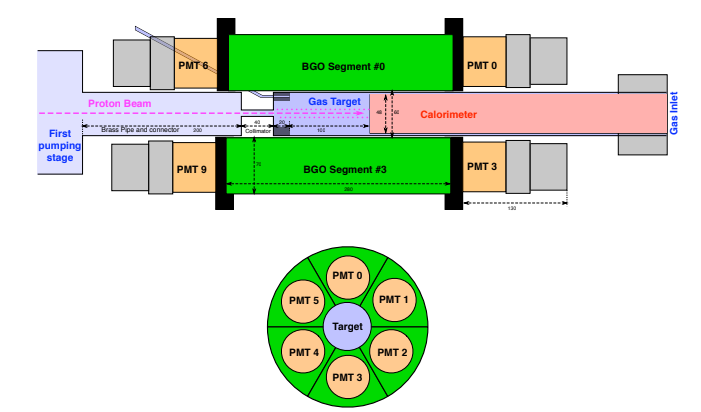
\includegraphics[width=\textwidth]{img/BGO.png}%solo parte inferiore, a voce
			\captionof{figure}{Rappresentazione schematica del rivelatore BGO. In alto una sezione sagittale, in basso una sezione trasversale.}
		\end{column}
	\end{columns}
\end{frame}


\begin{frame}{Efficienza}
	\begin{itemize}
			\item L'efficienza di uno scintillatore è il rapporto tra il numero di conteggi prodotti da esso e il numero di conteggi prodotti dalla sorgente:
			
			\begin{equation}
					\varepsilon = \dfrac{N_{\gamma}}{N_{int}}
				\end{equation}
			
			\item Si tratta pertanto di quanti fotoni lo strumento "vede" rispetto al totale
			\item Invertendo l'equazione possiamo ricavare $N_{int}$, per poi trovare la sezione d'urto
		\end{itemize}
\end{frame}


\begin{frame}{Tempo vivo/morto}
	\begin{itemize}
		\item Ogni strumento è elettronicamente vincolato a processare il segnale in ingresso
		\item Questo può richiedere fino a ns
		\item Un fotone in arrivo durante questo intervallo di tempo non può essere quindi rilevato
		\item Alla fine della misura verrano osservati meno fotoni di quelli effettivamente giunti allo strumento, perché quest'ultimo è attivo solo per una parte di tempo rispetto al totale della misura.
		\item L'intervallo in cui lo strumento è attivo e pronto a ricevere nuovi segnali è il \emph{tempo vivo}.
	\end{itemize}
\end{frame}
\begin{frame}{Risultati del fit}
	\begin{table}[ht]
		\centering
		\resizebox{0.7\textwidth}{!}{
			\begin{tabular}{@{}cccc@{}}
				\toprule
				Canale & Conversione [keV/CHN] \\ \midrule
				CHN1 & 1.1863 \(\pm\) 0.0009 \\
				CHN2 & 1.1659 \(\pm\) 0.0013 \\
				CHN3 & 1.3550 \(\pm\) 0.0019 \\
				CHN4 & 1.2676 \(\pm\) 0.0006 \\
				CHN5 & 1.2574 \(\pm\) 0.0010 \\
				CHN6 & 1.1388 \(\pm\) 0.0014 \\
				\bottomrule
		\end{tabular}}
	\end{table}
\end{frame}	

\begin{frame}{Caratterizzazione in energia}
	\begin{itemize}
			\item La caratterizzazione in energia è effettuata utilizzando due sorgenti radioattive: $^{60}$Co e $^{137}$Cs.
		\end{itemize}
\end{frame}

\begin{frame}{$^{60}$Co}%parlare sullo schema
	
	
	\begin{itemize}
		\item<1-> Il $^{60}$Co decade tramite decadimento $\beta^{-}$ (99.75\%) in $^{60}$Ni ed emette due raggi gamma di energie 1.17 MeV e 1.33 MeV.
		\item<2-> Ha il vantaggio di emettere raggi gamma ad alta intensità con un'emivita relativamente lunga di 5.27 anni. 
		\item<3-> Trova applicazione nella radioterapia del cancro.
	\end{itemize}
	
	\centering
	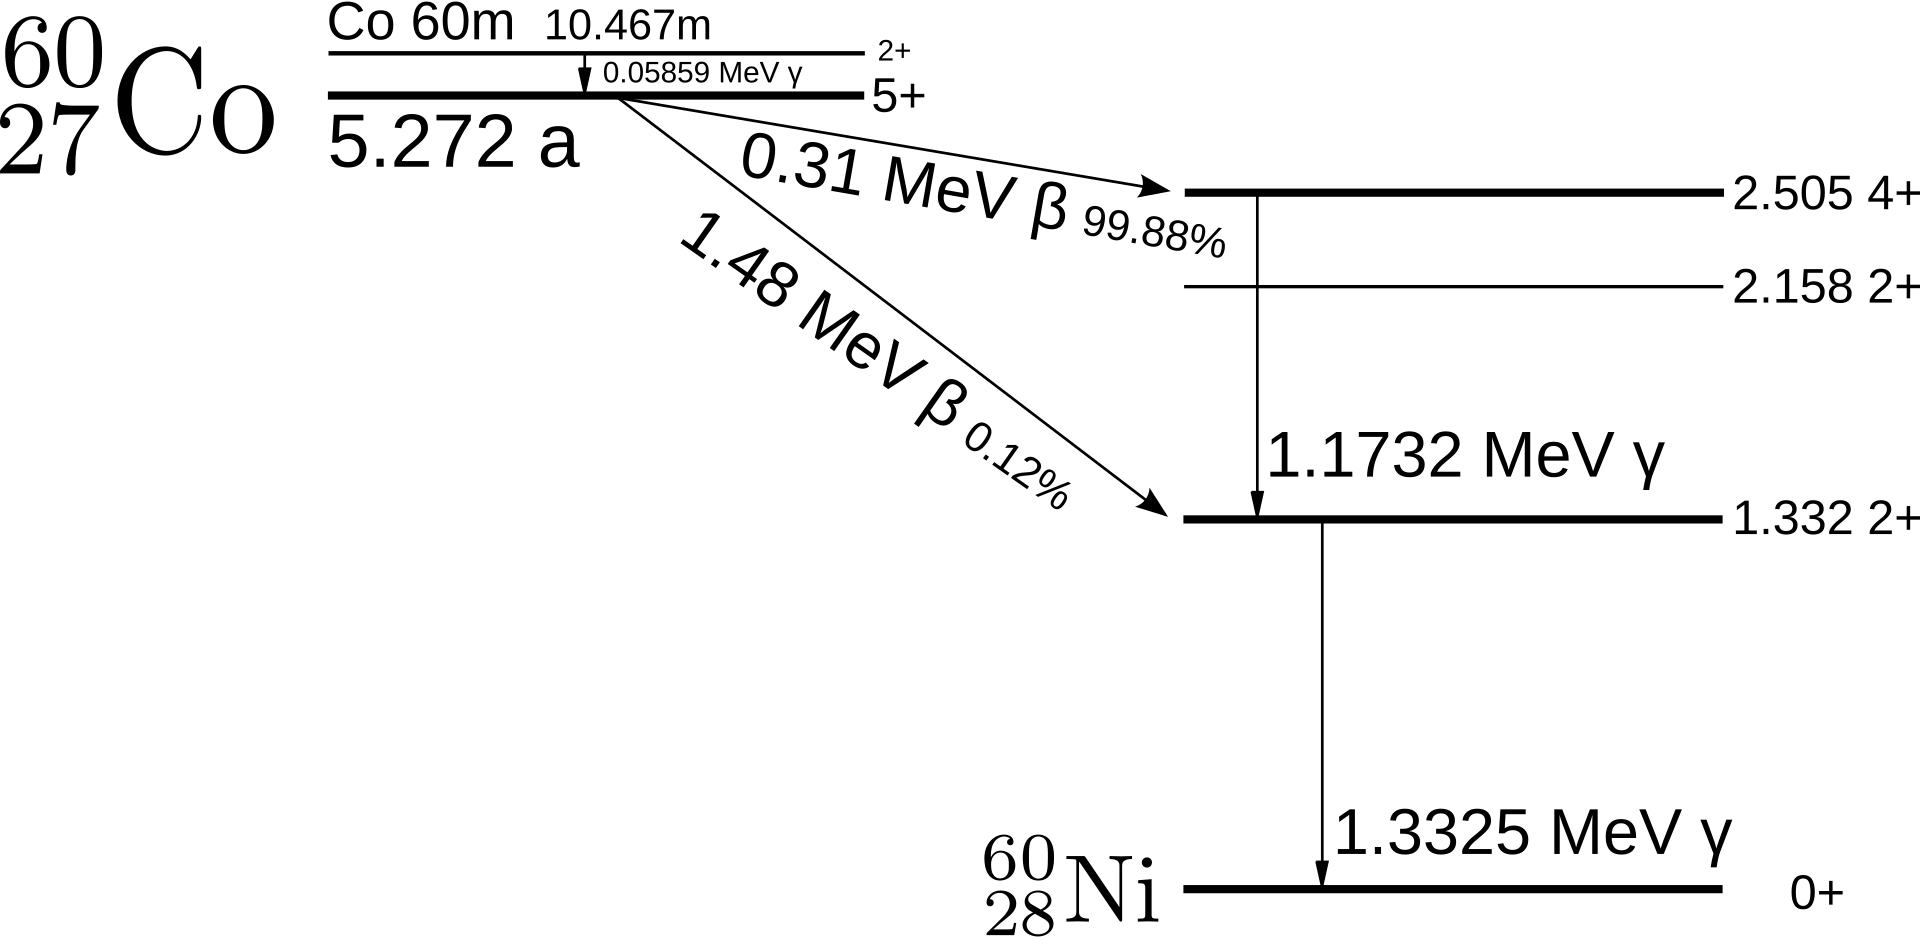
\includegraphics[width=0.5\textwidth]{img/Cobalt-60m-decay.png}
	\captionof{figure}{Schema di decadimento del $^{137}$Cs.}
	
\end{frame}



\begin{frame}{$^{137}$Cs}
	\begin{itemize}
		\item<1-> Il $^{137}$Cs decade sempre tramite decadimento $\beta^{-}$.
		\item<2-> Il 94.6\% dei decadimenti hanno come prodotto uno stato metastabile del $^{137}$Ba. 
		\item<3-> Questo stato eccitato emette l'85\% delle volte raggi gamma di 661.7 keV decadendo nello stato fondamentale del $^{137}$Ba (tutti i raggi gamma provenienti dal $^{137}$Cs sono prodotti così).
	\end{itemize}
	\centering
	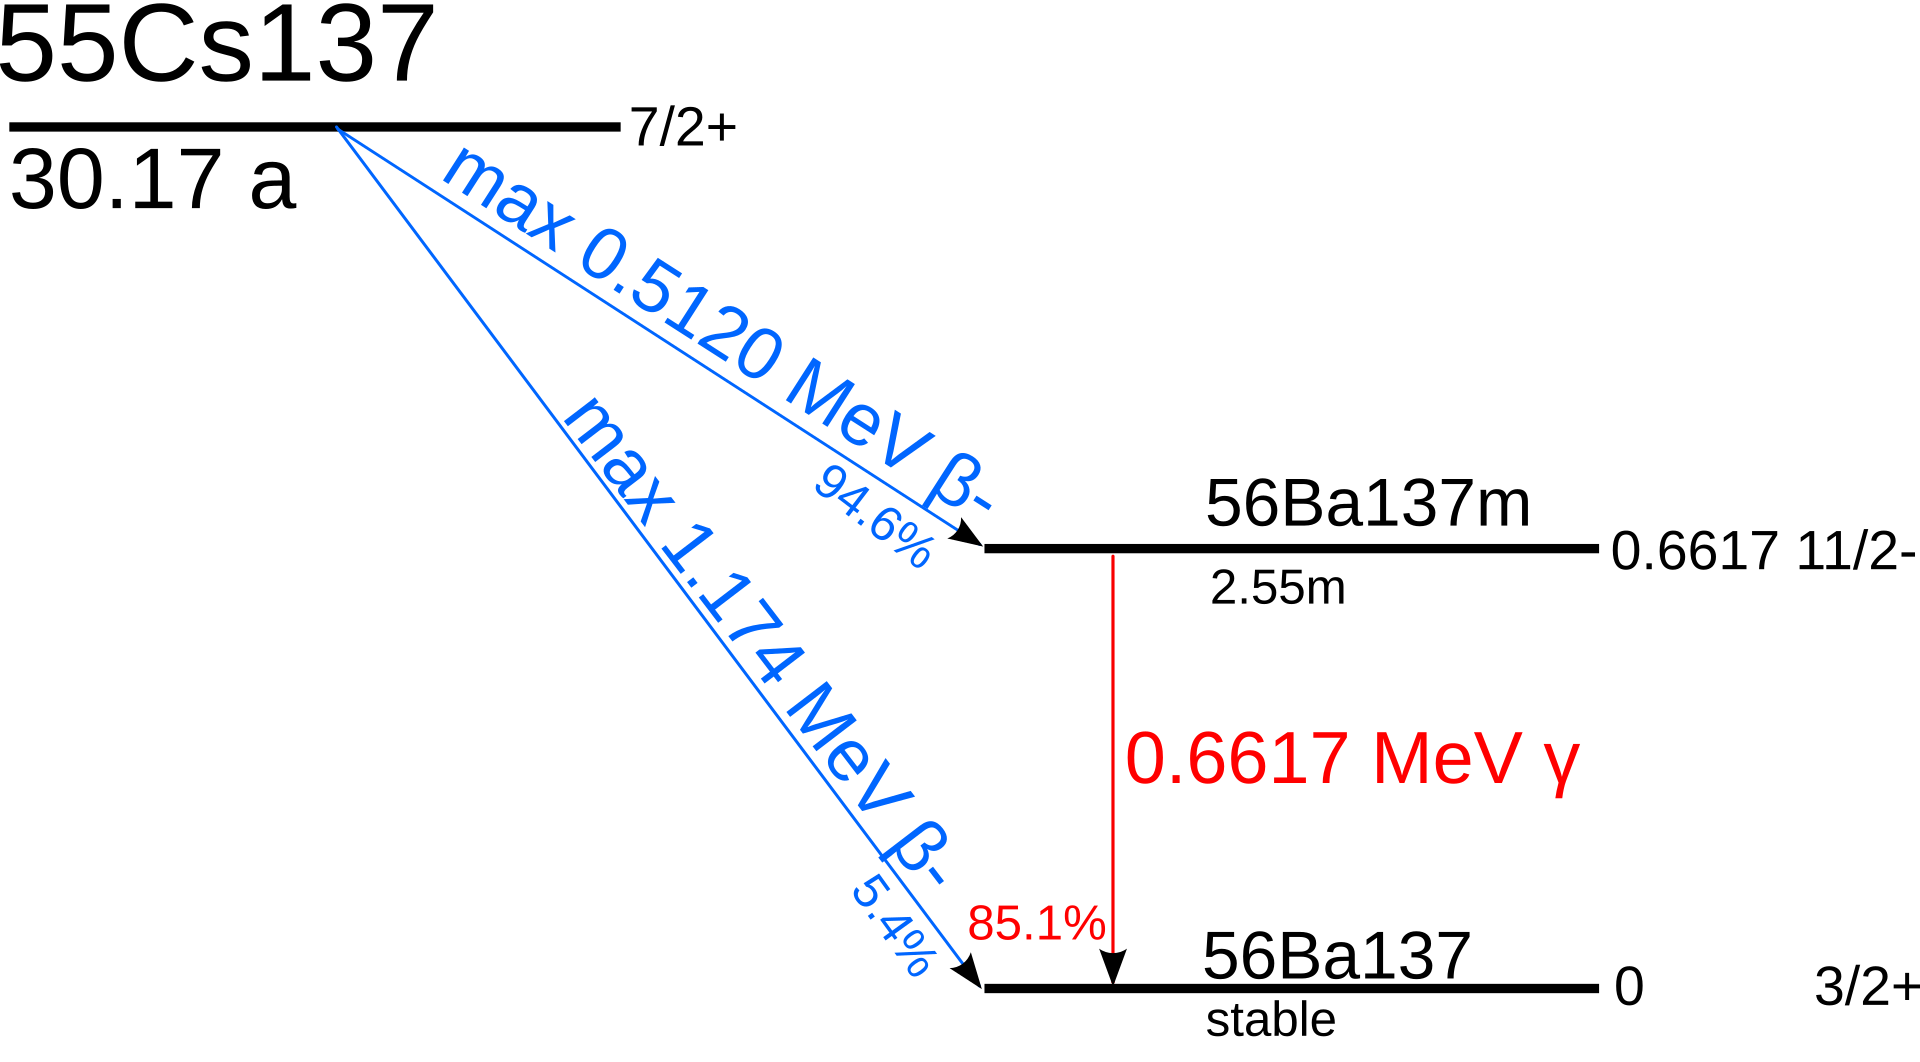
\includegraphics[width=0.5\textwidth]{img/Cs-137-decay.png}
	\captionof{figure}{Schema di decadimento del $^{137}$Cs.}
\end{frame}

\begin{frame}{\texttt{ROOT}}
	\begin{itemize}
		\item L'analisi dati dell'esperimento è compiuta in \texttt{ROOT}
		\item Il vantaggio di utilizzarlo è una discreta ottimizzazione per quanto riguarda l'analisi di grandi moli di dati grazie al formato file \texttt{.root}
		\item Si utilizza principalmente in ambito di fisica delle particelle
	\end{itemize}
\end{frame}


\begin{frame}{Struttura dei dati}
	\begin{itemize}
			\item I dati ricavati sono contenuti in file \texttt{.root}
			\item Ogni file \texttt{.root} contiene 8 istogrammi, con indici da 0 a 7, di conteggi
			\item L'istogramma 0 contiene il pulser, utilizzato per calcolare il tempo vivo dello scintillatore
			\item Gli istogrammi da 1 a 6 sono i singoli spicchi del BGO
			\item L'istogramma 7 è la corrente del fascio incidente sul BGO
		\end{itemize}
\end{frame}

\begin{frame}{Picco somma}
	\begin{itemize}
		\item Può accadere che lo strumento riveli due fotoni emessi dallo stesso evento contemporaneamente
		\item In tal caso, viene registrato come un unico fotone, ma con energia pari alla somma delle energie dei fotoni 
	\end{itemize}
\end{frame}

\begin{frame}{Residui}%mettere energie sull'asse X
	\begin{columns}%a voce sui residui
		\begin{column}{0.4\textwidth}
			\begin{itemize}
				\item<1-> I residui sono la differenza tra i valori in energia noti e quelli assunti dalla retta
				\item<2-> Sono una rappresentazione della bontà della calibrazione
				\item<3-> In generale una calibrazione è buona se i residui non superano la decina di keV
			\end{itemize}
		\end{column}
		\begin{column}{0.5\textwidth}
			\centering
			\only<2->{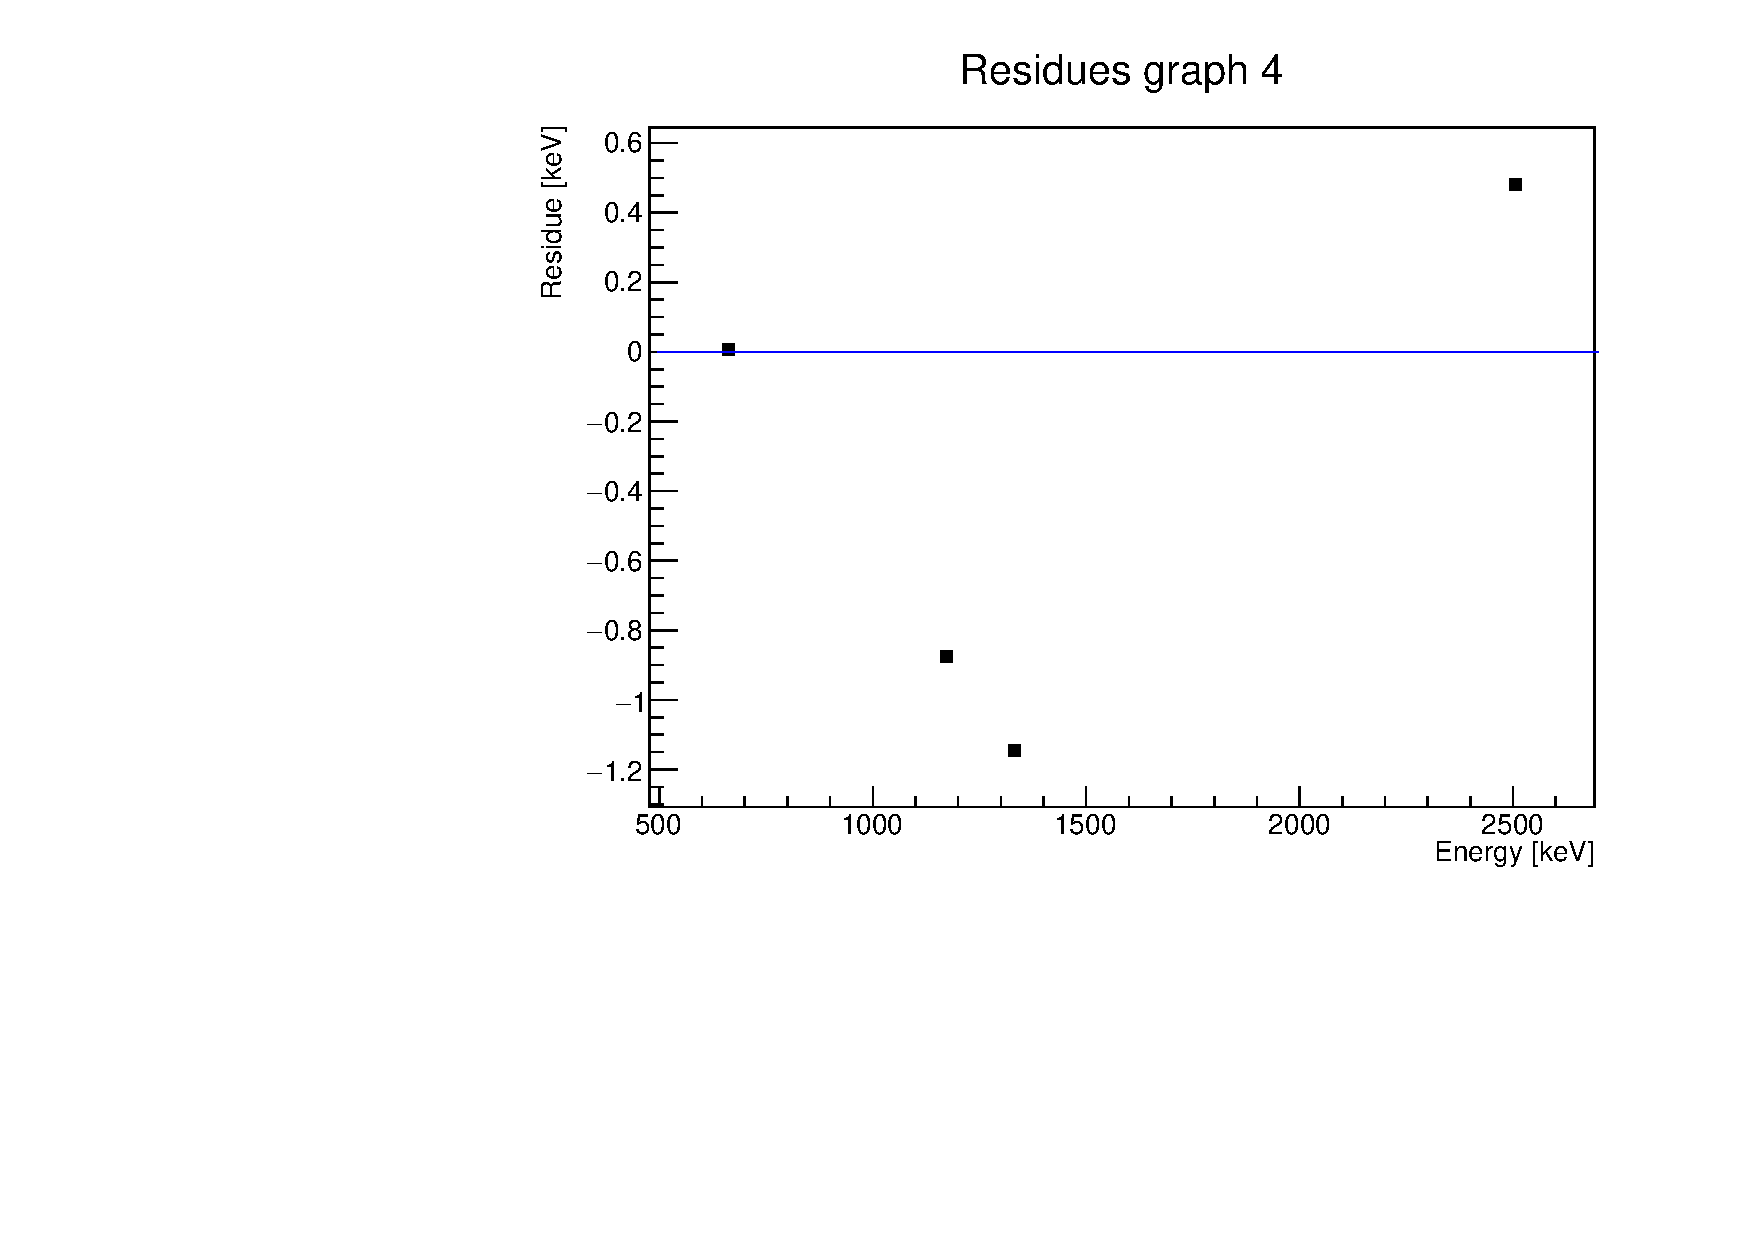
\includegraphics[width=0.9\textwidth]{img/residues0.pdf}}
		\end{column}
	\end{columns}
	
\end{frame}
\begin{frame}{Calcolo dell'efficienza}%si può dire tutto a voce, sulla immagine del picco senza fit (dall'altra parte mettere immagine con fit)
	\begin{itemize}
		\item Per il calcolo dell'efficienza è necessario trovare il numero di conteggi nei picchi gaussiani. Si possono applicare due metodi diversi per trovarlo:
	\end{itemize}
	\hrule height 0.3mm \vspace{2mm}
	
	\begin{columns}
		\column{0.5\textwidth}
		\uncover<2->{\centering \emph{Trapezio} 
			\begin{itemize}
				\item Metodo geometrico
				\item Consiste nell'isolare la regione del picco e rimuoverne il fondo trapezoidale
				\item Adatto solo per il cesio: i due picchi del cobalto non sono sufficientemente risolti dallo strumento
		\end{itemize}}
		
		\column{0.5\textwidth}
		\uncover<3->{\centering \emph{Parametrico}
			\begin{itemize}
				\item Metodo che sfrutta i parametri del fit
				\item Il coefficiente di normalizzazione del picco gaussiano è il numero di conteggi nel picco
				\item Adatto per cesio e cobalto
		\end{itemize}}
	\end{columns}
	
\end{frame}


%ricavo perché importante per sez d'urto
\begin{frame}{Efficienza}
	\begin{itemize}%discorso a voce, lasciare formula
		%		\item<1-> Nel caso dei nostri istogrammi, composti da un picco gaussiano centrato su un'energia caratteristica e un fondo di \emph{bremsstrahlung}, l'efficienza si può stimare nel modo seguente:
		%		%attività spiegata qua, tempo vivo dopo
		%		\begin{equation}
			%			\varepsilon = \dfrac{N_{cont.}}{A(t*) \Delta t}
			%		\end{equation}
		%	
		%		\visible<2->{dove $N_{cont.}$ è il numero di conteggi del picco gaussiano sottraendone il fondo, $A(t*)$ è l'attività calcolata al momento della misura, $\Delta t$ è il tempo "vivo" dello strumento.}
		\item<1-> L'efficienza è un fattore fondamentale per ricavare la sezione d'urto
		\item<2-> Si può stimare dalla formula:
		
		\begin{equation}
			\varepsilon = \dfrac{N_{cont.}}{A(t*) \Delta t}
		\end{equation}
		
		\item<3-> L'attività è calcolata al momento della misurazione. %magari discorso sulla legge esponenziale a voce
		
	\end{itemize}
\end{frame}

\begin{frame}{Calcolo dell'efficienza}
	\begin{columns}
		\begin{column}{0.5\textwidth}
			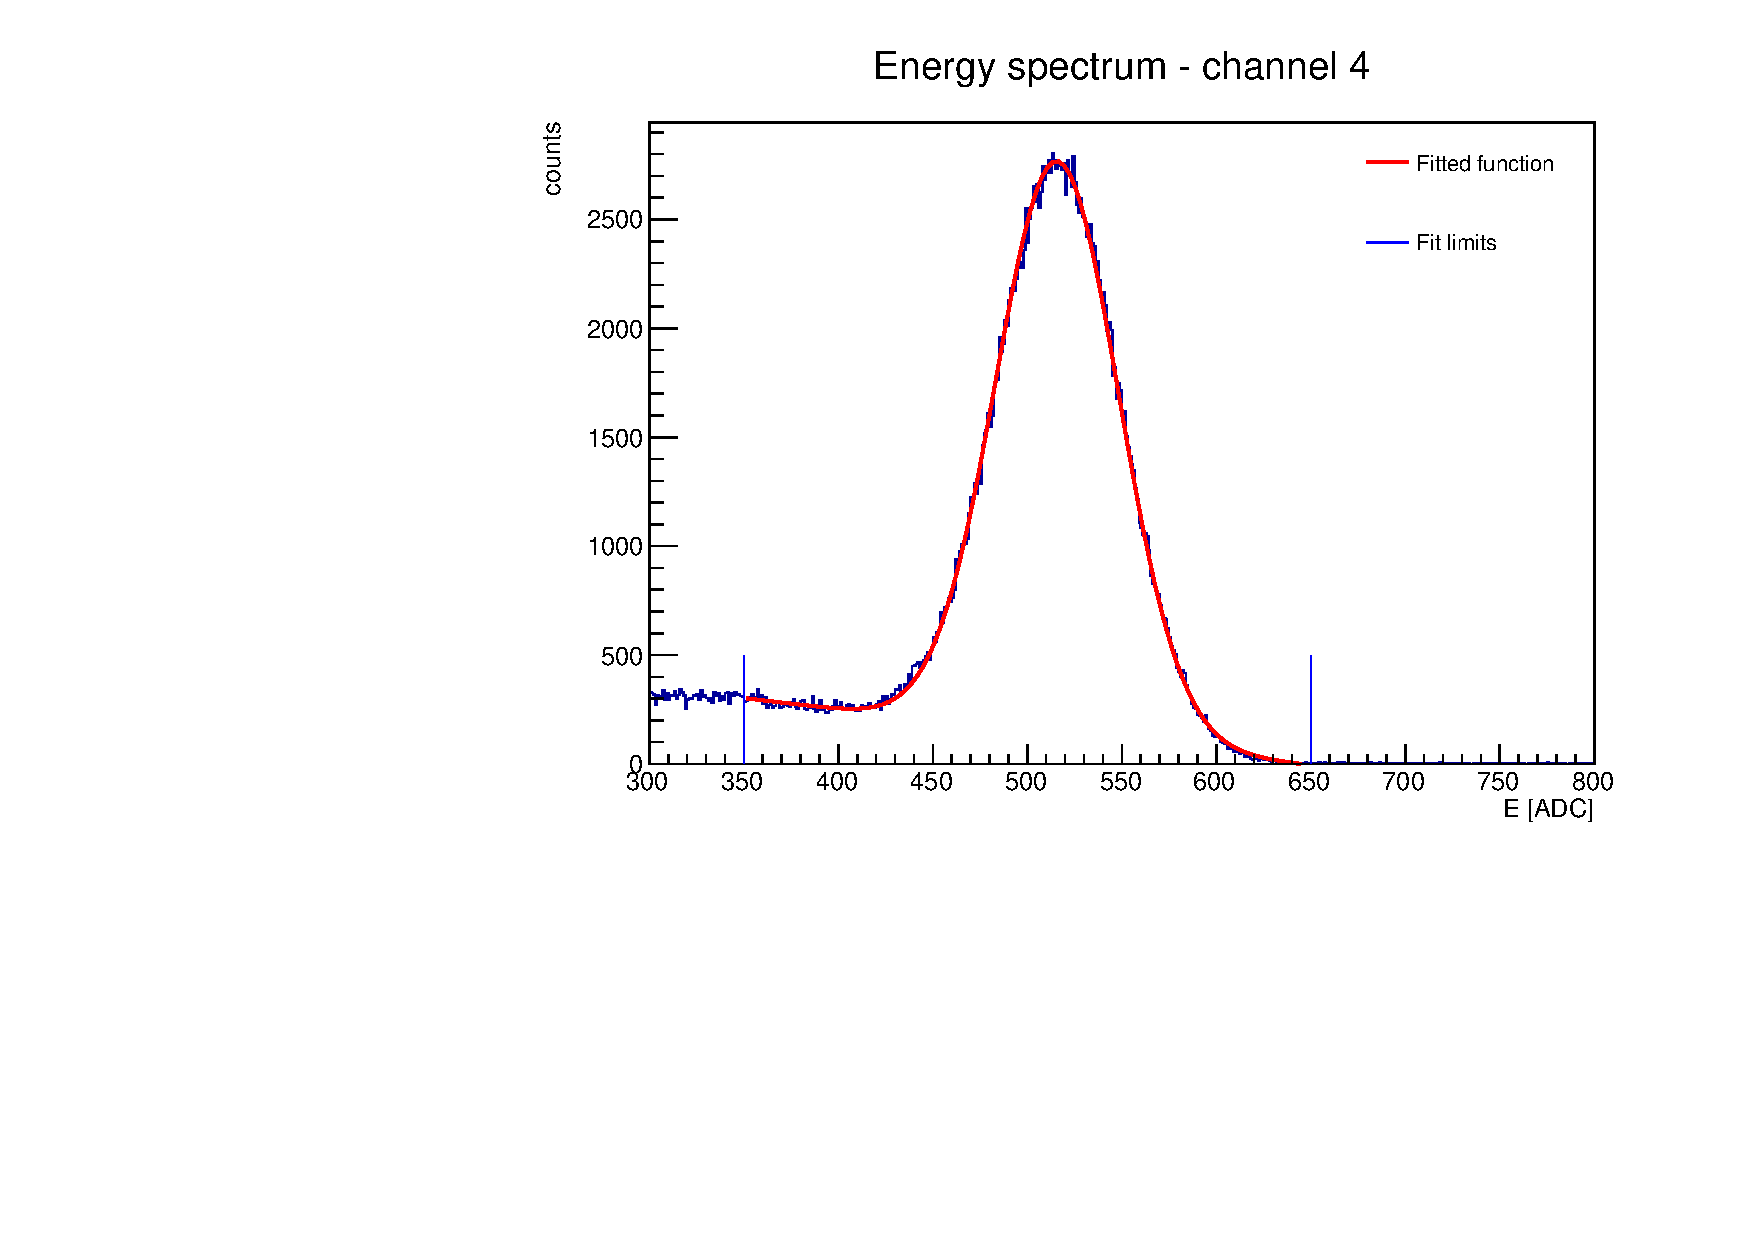
\includegraphics[width=\textwidth]{img/parameter.pdf}
		\end{column}
		\begin{column}{0.5\textwidth}
			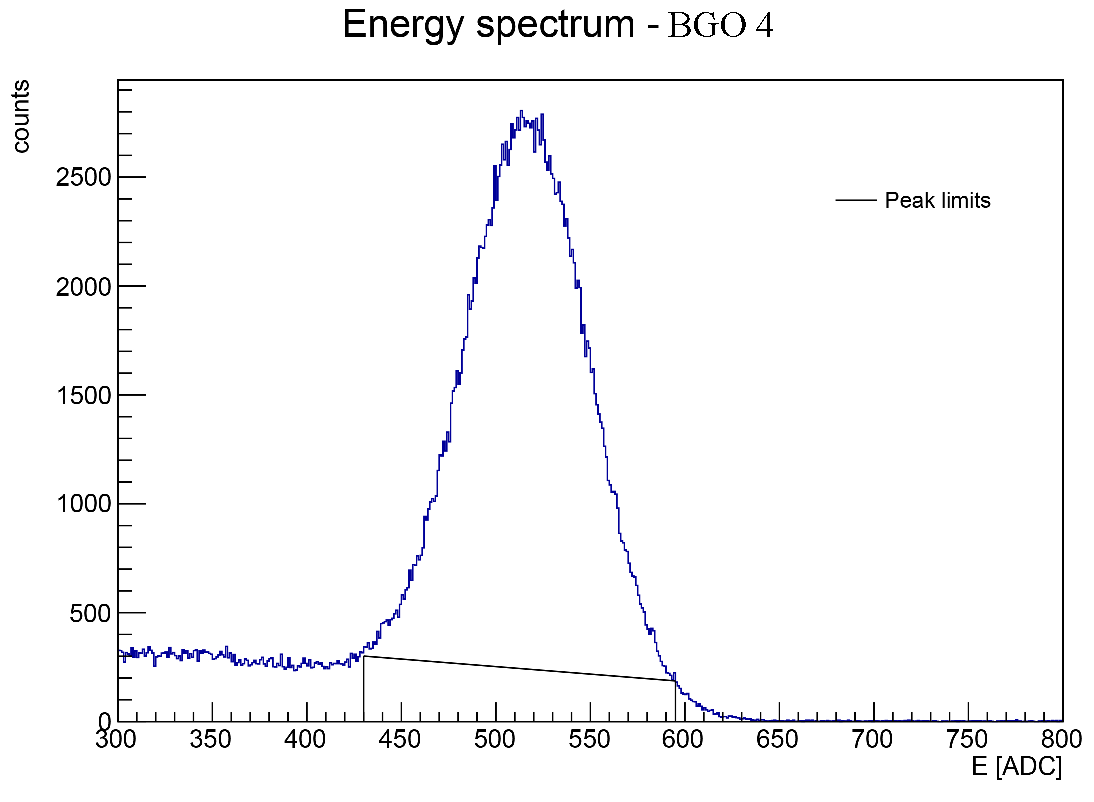
\includegraphics[width=\textwidth]{img/trapezoid.pdf}
		\end{column}
	\end{columns}
\end{frame}

\begin{frame}{Calcolo della calibrazione}
	\begin{itemize}
		\item La calibrazione viene effettuata sul file \texttt{run1775\_coinc.root}, con entrambe le sorgenti.
		\item \emph{Calibrare} uno scintillatore significa trovare il fattore di conversione da canali a energia.
		\item Per ogni spicchio del BGO si esegue un fit per trovare il valore dei picchi caratteristici e del picco somma in canali.
	\end{itemize}
\end{frame}

\begin{frame}{Risoluzione energetica}%inserire spettro simulato con ris inf e far veder come viene fuori con risoluzione dopo applicazione
		\begin{itemize}
				\item Le simulazioni contengono picchi di energia ideali, a cui non è stata applicata la risoluzione dello strumento
				\item Questa si può trovare eseguendo fit gaussiani sugli istogrammi in energia, anziché canali
				\item La risoluzione è il rapporto tra la deviazione standard del picco e la corrispondente energia nota
				\item Le risoluzioni si mettono su un grafico contro le corrispettive energie note, fittandovi una funzione:
				
				\begin{equation*}
						f(E) = a + \dfrac{b}{\sqrt{E}}
					\end{equation*}
			\end{itemize}
	%lasciare funzione fittata
\end{frame}
\begin{frame}{Pulser}
	\begin{columns}
		\begin{column}{0.5\textwidth}
			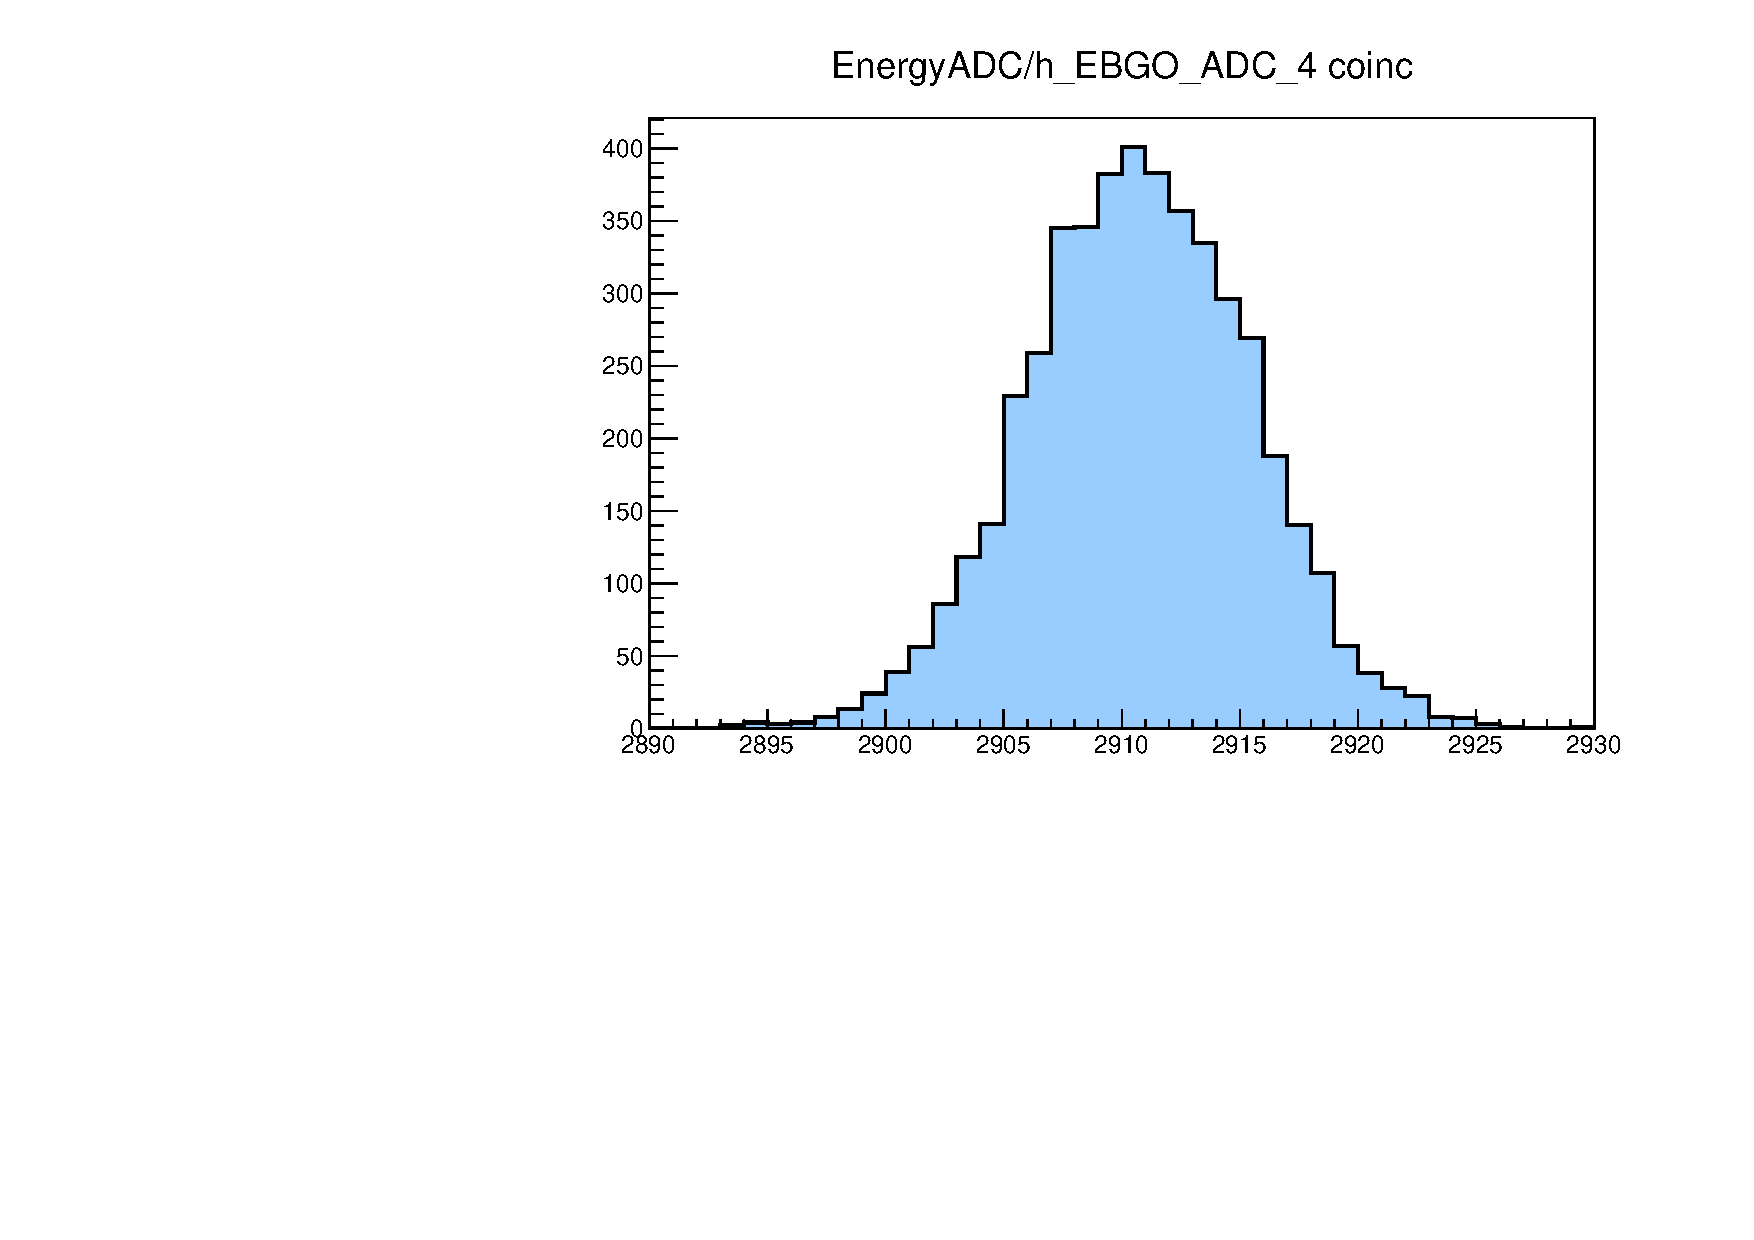
\includegraphics[width=\textwidth]{img/run1776_coinc_h_EBGO_ADC_4_COINC.pdf}
		\end{column}
		\begin{column}{0.5\textwidth}
			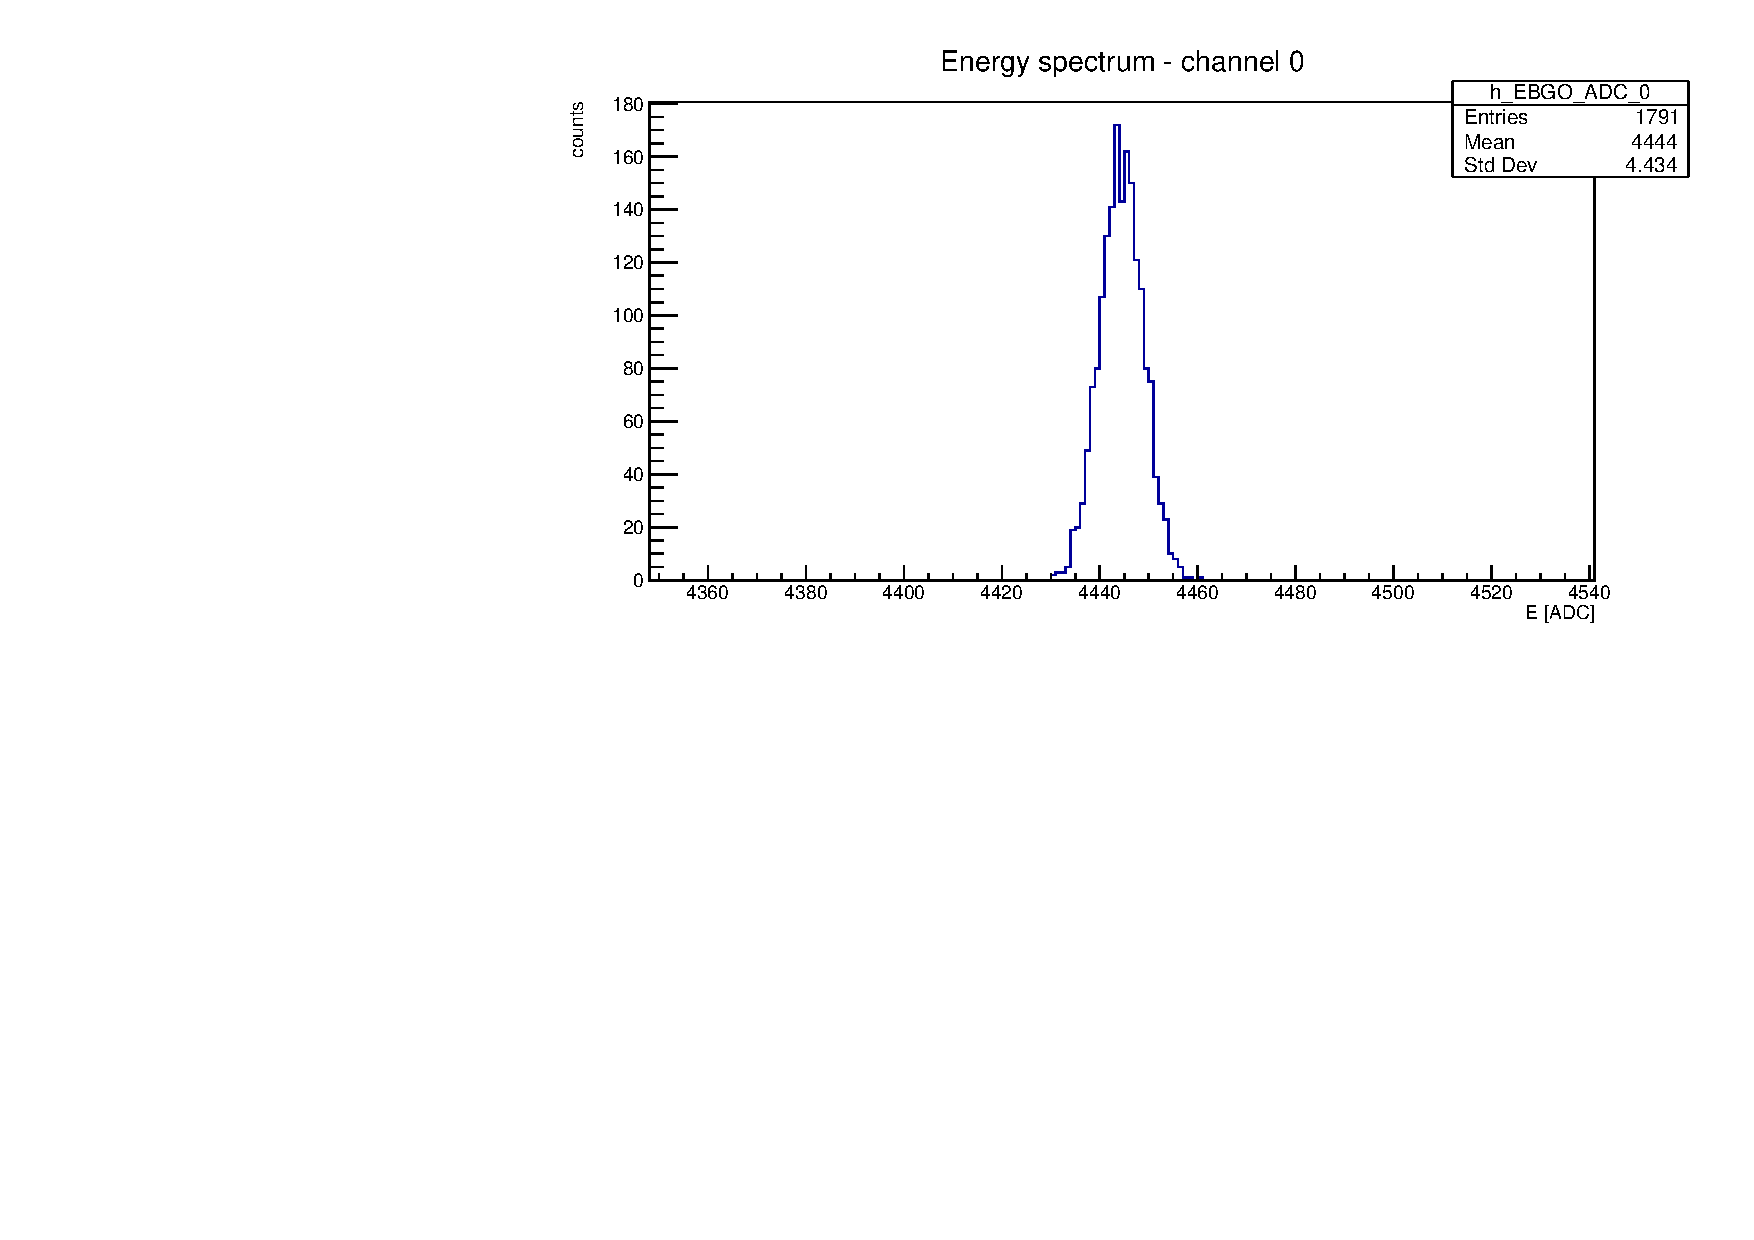
\includegraphics[width=\textwidth]{img/pulser.pdf}
		\end{column}
	\end{columns}
\end{frame}

\end{document}

